\chapter{高輝度LHC-ATLAS実験に向けたTGC検出器システムのアップグレード}
\label{chap_TGC}

% この章では、自分の研究に関連する分野の歴史や現状について説明したり、研究を展開する上で重要となる知識の解説を行います。ここで使用している見出し「ガンマ線天文学…」はあくまで例ですが、もしCherekov Telescope Array(CTA)計画\footnote{省略語は必ず正式名称を先に書き、省略系は丸括弧に入れます。省略語はあくまで「以降このように略す」という用途だからです。また、日本語文章中で使う丸括弧は ()ではなく()です。}に携わる院生の書く修士論文であれば、ガンマ線天文学や宇宙線物理学全般について、現行望遠鏡とガンマ線観測の原理について、またCTA計画についての記述がこの章では期待されます。

% 場合によっては「序論」と合体させても良いですが、本章は比較的長くなり結論に直結しない情報もたくさん出てくるため、独立した章である方が読者は読みやすいでしょう。

% またこの章が長くなるときには、例えば「ガンマ線天文学」と「CTA計画」のように、2つの章に分割するというのも良いと思います。\footnote{注意書きの練習です。}

\section{LHC-ATLAS実験におけるTGC検出器}
本節では本研究のテーマである、Thin Gap Chamber (TGC) 検出器について説明する。それに先んじて、ATLAS検出器で使われる座標系と、ATLAS検出器における磁場構造について説明する。

\subsection{ATLAS実験における座標系}
\label{subsec_ATLAScordination}
ATLAS実験では主に2種類の座標系が用いられる。図\ref{ATLAScordination}にその概要を示す。1つ目の座標系である直交座標系は、原点を検出器中心に取りLHCの中心方向を$x$、地上方向を$y$に取った右手系で定義する。この時、$z$軸はビーム軸方向に沿って定義される。$z>0$ の領域をA side、$z<0$の領域をC sideと呼ぶ。2つ目の座標系である円筒座標系は、ビーム軸を中心とした方位角方向を$\phi$、ビーム軸からの天頂角方向を$\theta$、同型方向を$R$と定義する。また、$\theta$ 方向を表す変数として、擬ラピデティ  (Pseudorapidity)
\begin{equation}
    \eta = -\ln(\mathrm{tan}\frac{\theta}{2})
\end{equation}
を定義し、粒子の四元運動量を記述する際\footnote{$\eta$はハドロンコライダーで生じる物理現象を説明する際によく利用される。2粒子間の$\eta$の差は$z$軸方向のブーストに対してローレンツ不変であり、始状態の粒子の$z$方向の運動量に関わらず崩壊事象を統一的に記述することができる。}やビーム衝突点から見た時の各検出器の立体角を議論する際に利用する。本研究で扱うミューオンシステムの議論でも$\eta$を利用し、|$\eta$| < 1.05の円筒側面領域をバレル領域 (Barrel) 、|$\eta$| > 1.05の円筒底面領域をエンドキャップ ( Endcap) と区別する。

ATLAS実験では粒子の状態を表す物理量として$z$軸垂直方向の運動量 (横方向運動量、\pt) やエネルギー (横方向エネルギー、$E_{\mathrm{T}}$) を利用する。
高エネルギーの陽子陽子衝突は、陽子の内部構造であるパートン同士の衝突であり、その担う運動量の差により衝突重心系は実験室系では$z$軸方向にローレンツブーストされている。一方で横方向の運動量は (交差角の効果や、フェルミ運動量を除けば) 実験室系で厳密にゼロとなる。終状態粒子の運動量の$z$軸方向の成分はパートン同士の運動量の非対称による寄与が大きく、パートン同士の衝突重心系の全エネルギーの良い指標にはならない。一方、で横方向の運動量はパートン同士の衝突重心系の全エネルギーの良い指標となるため、横方向運動量や横方向エネルギーが事象選別の重要な指標となる。オンライン事象選別であるトリガーでも横方向運動量、横方向エネルギーを指標にして興味のある事象を選択する。

\begin{figure} 
\centering
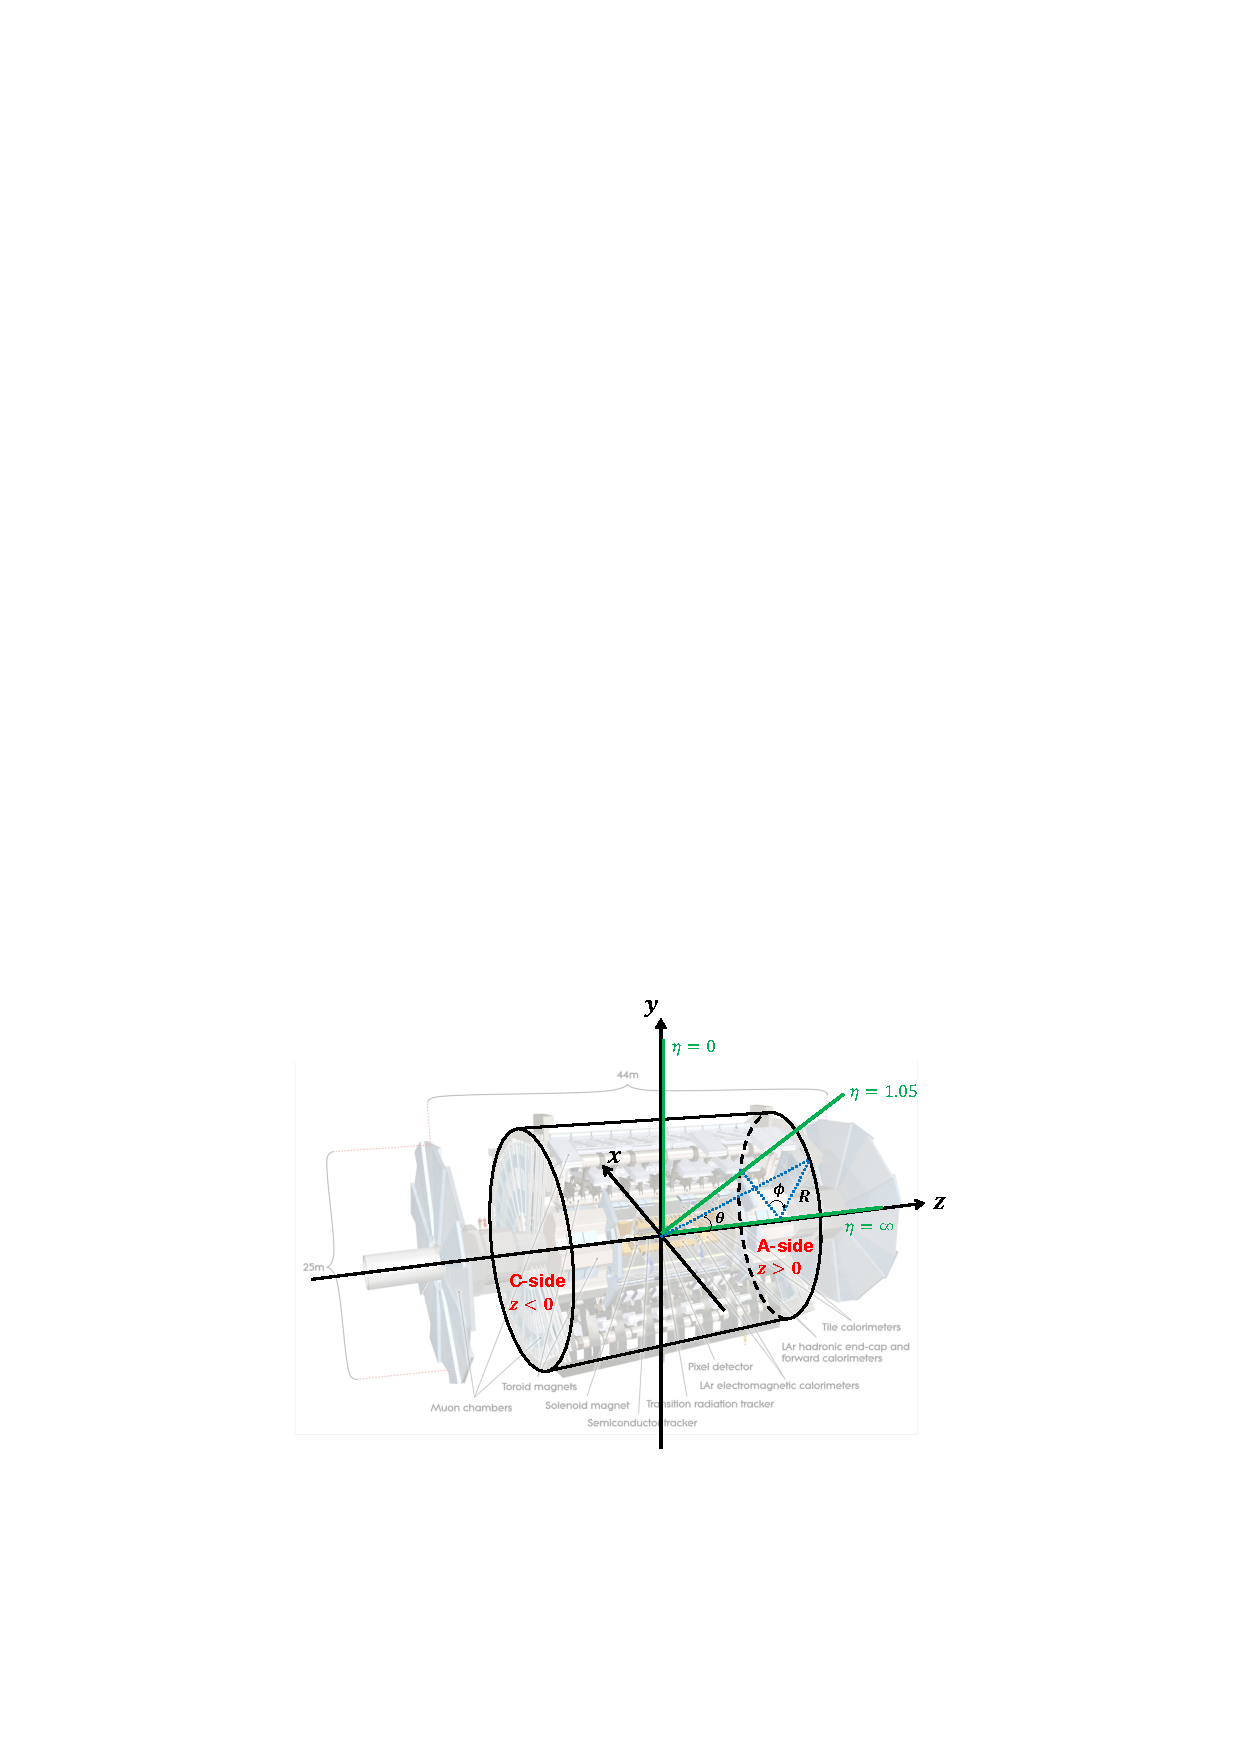
\includegraphics[width=16cm]{fig/Intro/ATLAScordination.pdf}
\caption[ATLAS検出器における座標系]{ATLAS検出器で用いられる座標系。直交座標系は、原点を検出器中心に取りLHCの中心方向を$x$、地上方向を$y$に取った右手系で定義する。$z>0$をA side、$z<0$をC sideと呼ぶ。円筒座標系は、ビーム軸を中心とした方位角方向を$\phi$、ビーム軸からの天頂角方向を$\theta$、同型方向を$R$と定義する。最外層のミューオンシステムは|$\eta$| = 1.05でバレル領域とエンドキャップ領域に分かれる。}
\label{ATLAScordination}
\end{figure}

\subsection{ATLAS検出器における超伝導磁石}
\label{subsec_magnet}
ATLAS検出器では荷電粒子の運動量を測定するため、2種類の超伝導磁石が設置されている。図\ref{ATLASmagnet}に超伝導磁石の配置を示す。1つ目は、内部飛跡検出器内で荷電粒子を曲げるのに利用されるソレノイド磁石である。ソレノイド磁石は内部飛跡検出器とカロリメーターの間の領域に設置され、$z$軸方向の磁場を生成する。2つ目は、内部検出器を透過してきたミューオンを曲げるのに利用されるトロイド磁石である。トロイド磁石はバレル部用とエンドキャップ部用で2種類用意される。バレル部とエンドキャップ部のトロイド磁石はそれぞれ$\phi$方向に8回対称の構造をとっており、互いの干渉を避けるため22.5度ずらして設置される。トロイド磁石は主に$\phi$方向の磁場を生成し、$\eta$方向に荷電粒子を曲げるが、磁石の構造によって磁場は場所ごとに不均一になっている。

\begin{figure} 
    \centering
    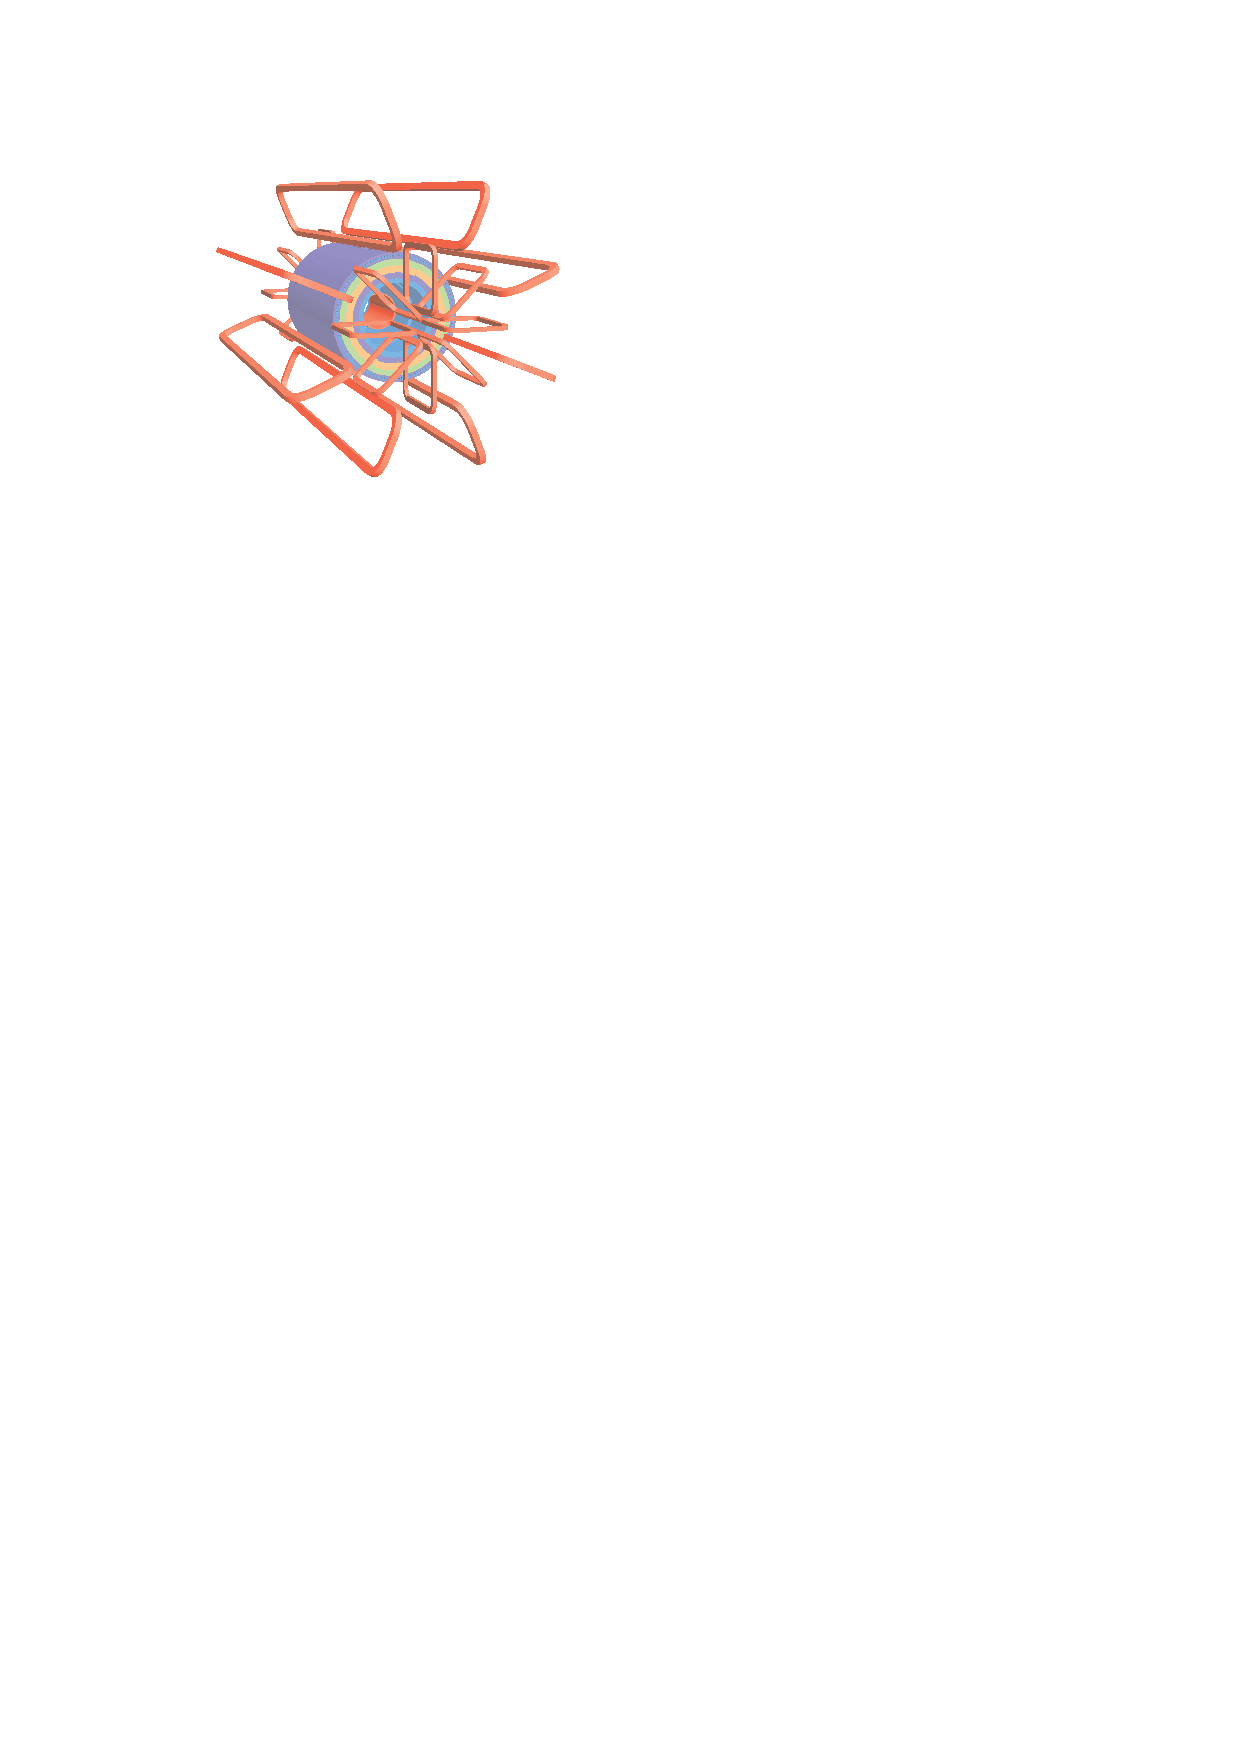
\includegraphics[width=12cm]{fig/Intro/ATLASmagnet.pdf}
    \caption[超伝導磁石の配置]{超伝導磁石の配置\cite{JINST:2008}。内部飛跡検出器を囲うようにソレノイド磁石が、カロリメーターの外側にトロイド磁石が設置されている。バレル部とエンドキャップ部のトロイド磁石はそれぞれ$\phi$方向に8回対称の構造をとっており、互いの干渉を避けるため22.5度ずらして設置される。}
    \label{ATLASmagnet}
\end{figure}

\subsection{ミューオンスペクトロメーター}
\label{subsec_Muonspectrometer}
ミューオンスペクトロメーターはATLAS検出器最外層に設置された検出器で、カロリーメーターを透過したミューオンの横方向運動量を測定する。ミューオンスペクトロメーターはトロイド磁場の構造に合わせて$\phi$方向に8回対称になっており、そのうちバレル部のトロイド磁石が位置する領域を Small sector、トロイド磁石間に位置する領域をLarge sectorと呼ぶ。ミューオンスペクトロメーターの全体像を図\ref{Muonspectrometer2}に示す。

高輝度LHC-ATLAS実験でエンドキャップ部ミューオントリガーに関わる検出器には、TGC検出器、New Small Wheel (NSW)、Resistive Plate Chamber (RPC)、Monitored Drift Tube (MDT) 、Tile カロリメーターがある。TGC検出器については後ほど詳述する。NSWはエンドキャップトロイド磁場の内側に設置されたトリガーおよび精密測定用のミューオン検出器であり、1.3 < |$\eta$| < 2.7の全$\phi$方向をカバーする。small-strip TGC (sTGC) とMicromegas (MM) の2種類の検出器を4層ずつ組み合わせた構造をしており、荷電粒子が通過した位置および飛跡の角度情報を取得する。RPCは |$\eta$| < 1.05のバレル領域に設置されたトリガー用のミューオン検出器である。直交するストリップで$\eta$と$\phi$の位置情報を読み出す。Run 3以降ではSmall sector にRPC BIS78 というエンドキャップ領域をカバーする検出器が設置され、エンドキャップミューオントリガーで利用される。MDTはバレル領域およびエンドキャップ領域に設置された精密測定用のミューオン検出器である。ドリフトチューブを6層または8層並べた構造をとっており、荷電粒子が通過した位置および飛跡の角度情報を再構成する。MDTはドリフト時間が長く、Run 3までは初段トリガーで用いることができなかったが、高輝度LHC-ATLAS実験からは拡張されるレイテンシーを活用して、初段トリガーにも用いられる。Tile カロリメーターは電磁カロリメーターの外側に設置されたハドロンカロリメーターであり、複数の層が重なった構造をとっている。最外層に到達する粒子のほとんどがミューオンであることを利用して、エンドキャップ領域のトリガー判定に用いられる。


\begin{figure}
\begin{minipage}[b]{1.0\linewidth}
\centering
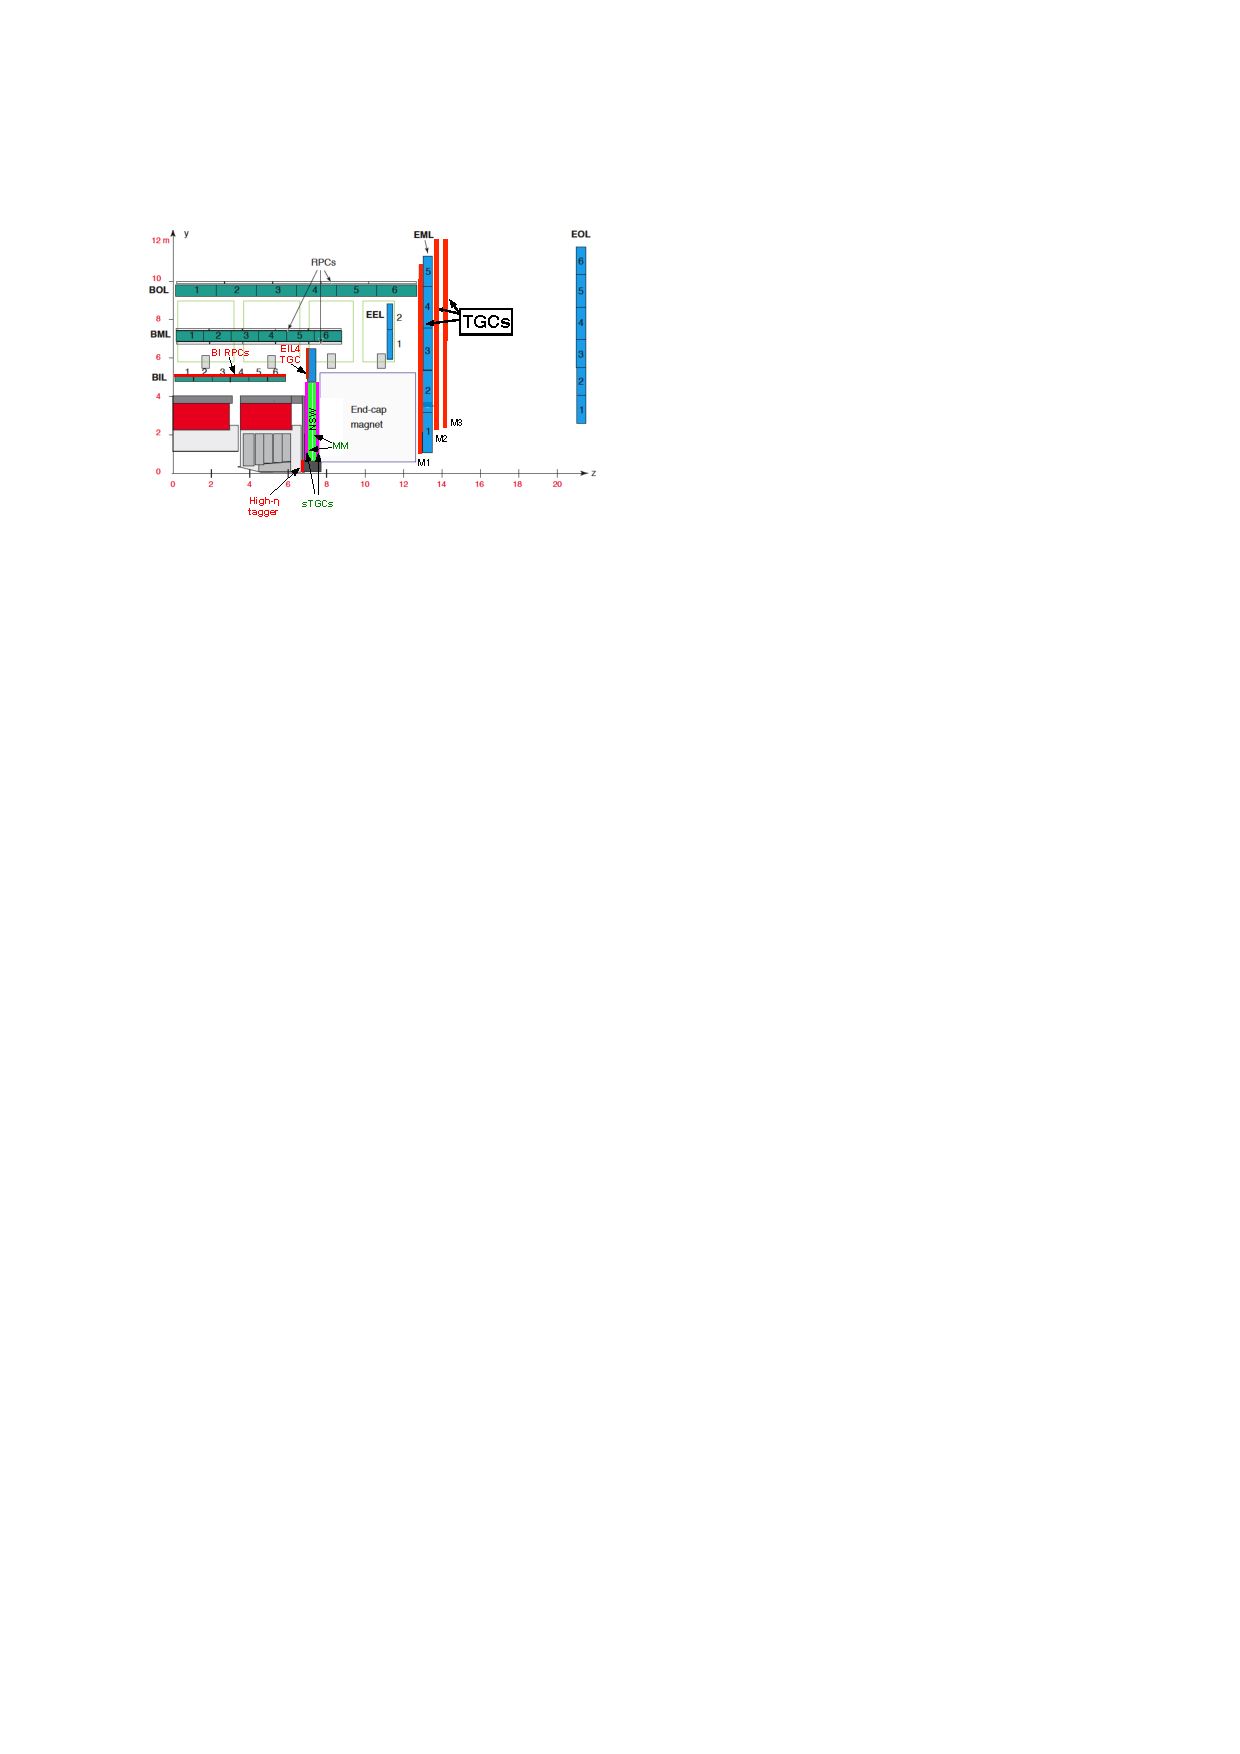
\includegraphics[width=16cm]{fig/Intro/MuonSpe_Large.pdf}
\subcaption{Large sectorでのミューオン検出器の配置}
\end{minipage}\\
\begin{minipage}[b]{1.0\linewidth}
\centering
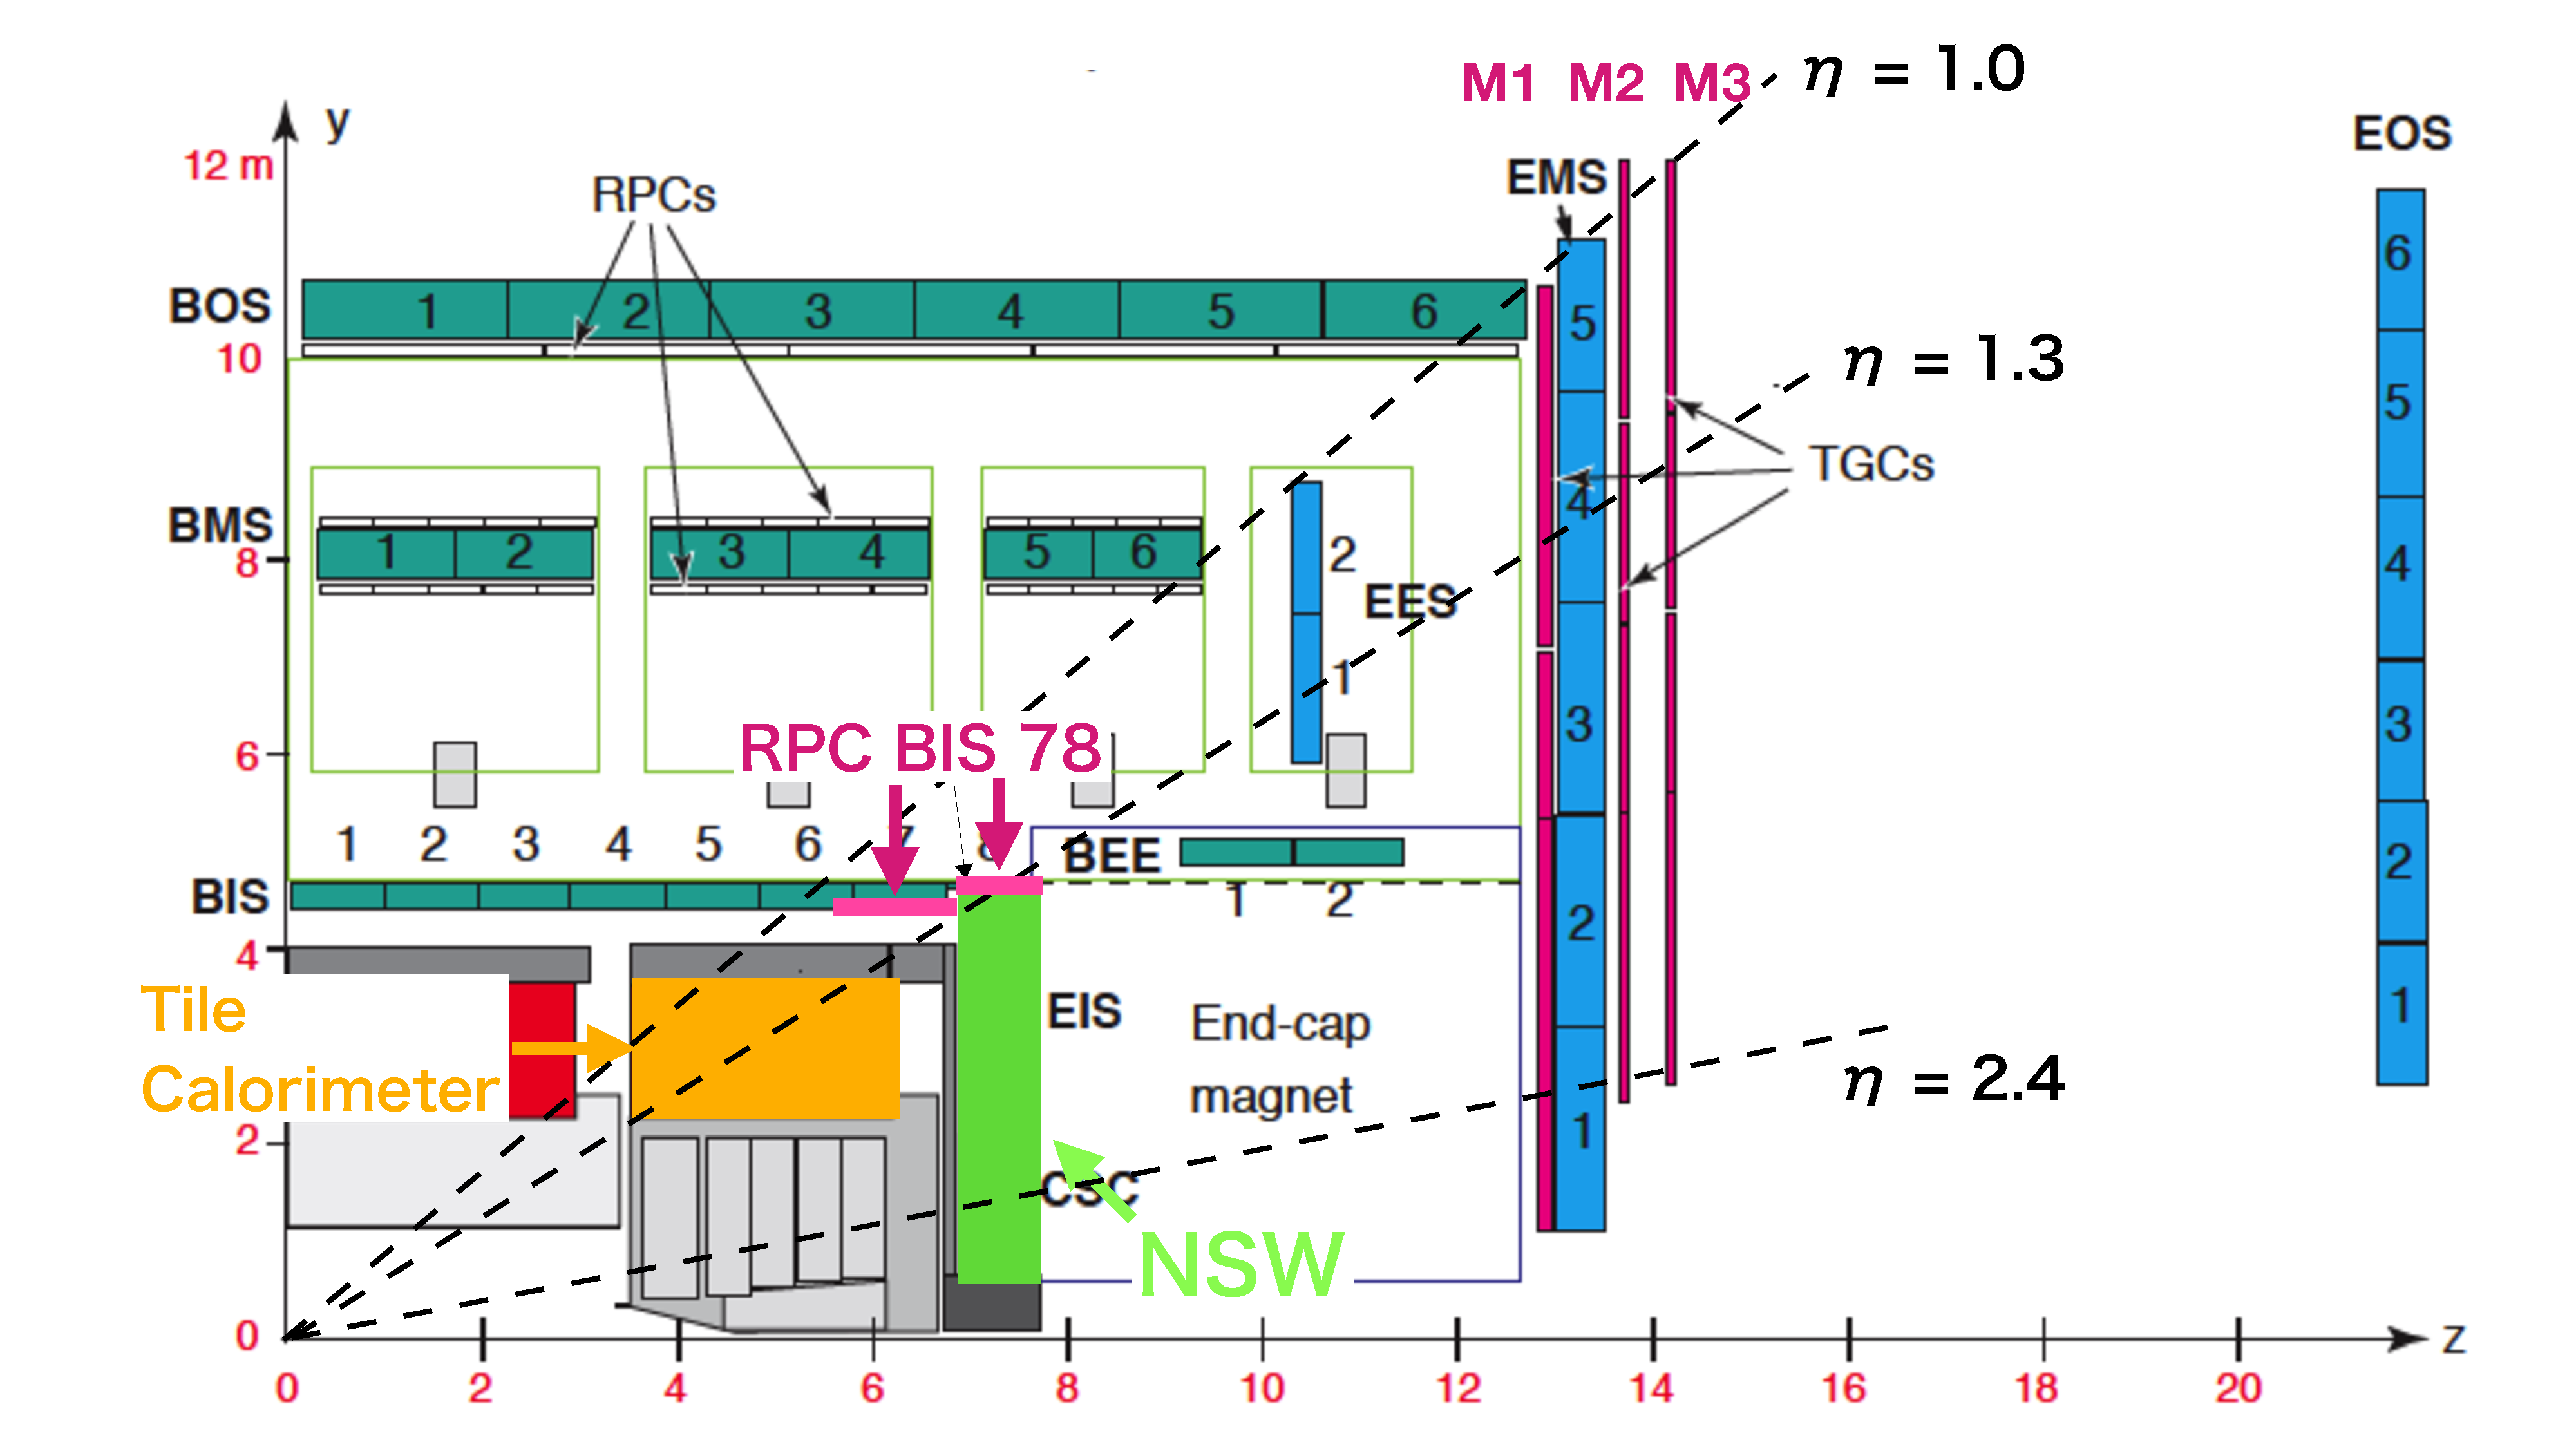
\includegraphics[width=16cm]{fig/Intro/MuonSpe_small.pdf}
\subcaption{Small sectorでのミューオン検出器の配置}
\end{minipage}%
\caption[高輝度LHC-ATLAS実験でのミューオンスペクトロメーターの$R$-$z$平面断面図]{高輝度LHC-ATLAS実験でのミューオンスペクトロメーターの$R$-$z$平面断面図\cite{tdr_phase2muon_2017017}。TGC BW 以外のミューオンスペクトロメーターはトロイドマグネットの磁場構造に合わせて8回対称になっており、$\phi$方向にLarge Sector、Small sectorという2種類のsectorに分かれている。エンドキャップ部のミューオントリガーには1.05 < |$\eta$| < 1.3の領域ではTGC、RPC BIS78、TGC EIL4、Tile カロリメーターが、1.3 < |$\eta$| < 2.4の領域ではTGCとNSWが用いられる。}
\label{Muonspectrometer2}
\end{figure}

\subsubsection*{TGC検出器}
TGC検出器は1.05 < |$\eta$| < 2.4のエンドキャップ領域に設置されたミューオントリガー用の検出器である。エンドキャップトロイド磁石より内側に位置するEndcap Innner  (EI) と外側に位置するBig Wheel  (BW) に大別される。TGC BWは$z$方向に3つのステーションが連なって構成され、衝突点に近い方からM1、M2、M3ステーションと呼ぶ (図\ref{Muonspectrometer2}参照)。各ステーションは2層または3層のガス層で構成されており、2層のものをDoublet、3層のものをTripletと呼ぶ。BWではM1がTriplet、M2、M3がDoubletになっている。

TGCチェンバーの構造を図\ref{TGC_structure}に示す。TGCはアノードワイヤー間隔が1.8 mm、アノードとGNDの間隔が1.4 mmであるMWPCである。ワイヤーは$R$方向、ストリップは$\phi$方向に直交して張られており、それぞれのヒット信号からミューオンが通過した2次元位置を検出することができる。ガス層には$\mathrm{CO_2}/n\text{-}\mathrm{C_5H_{12}}$が55:45で混合されたガスが充填されている。荷電粒子がTGCに入射すると、電磁相互作用によりガス分子が電離される。電離した電子はワイヤーに印加された2.8 kVの電圧によりワイヤー方向に集められ、ワイヤー付近に到達すると強い電場により電子雪崩を生じる。ワイヤーでは電子雪崩で生じた正イオンのドリフトが、ストリップではそれらの鏡像電荷が電流信号として検出される。

\begin{figure}
\begin{minipage}[b]{.4\linewidth}
\centering
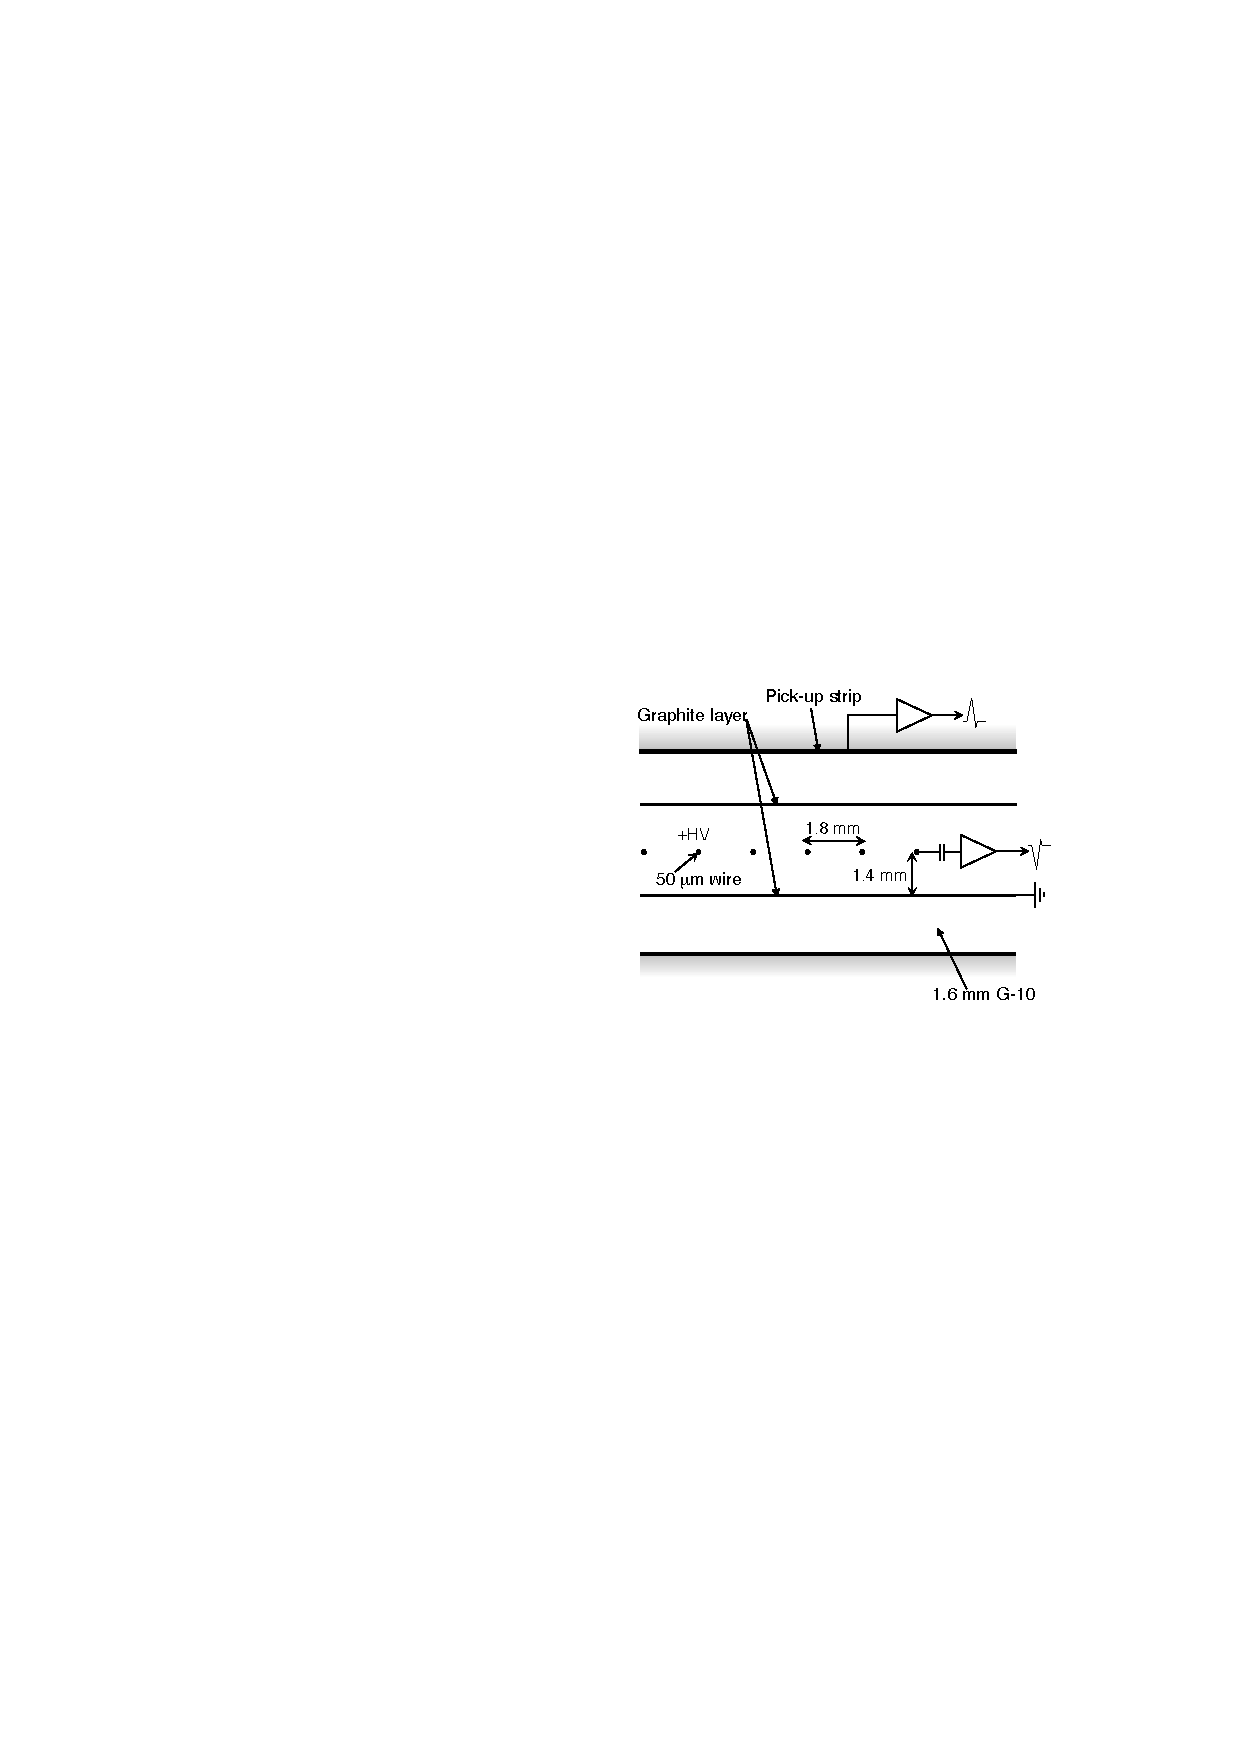
\includegraphics[height=5cm]{fig/Intro/TGC_structure.pdf}
\subcaption{TGCチェンバーの断面図}
\end{minipage}%
\begin{minipage}[b]{.6\linewidth}
\centering
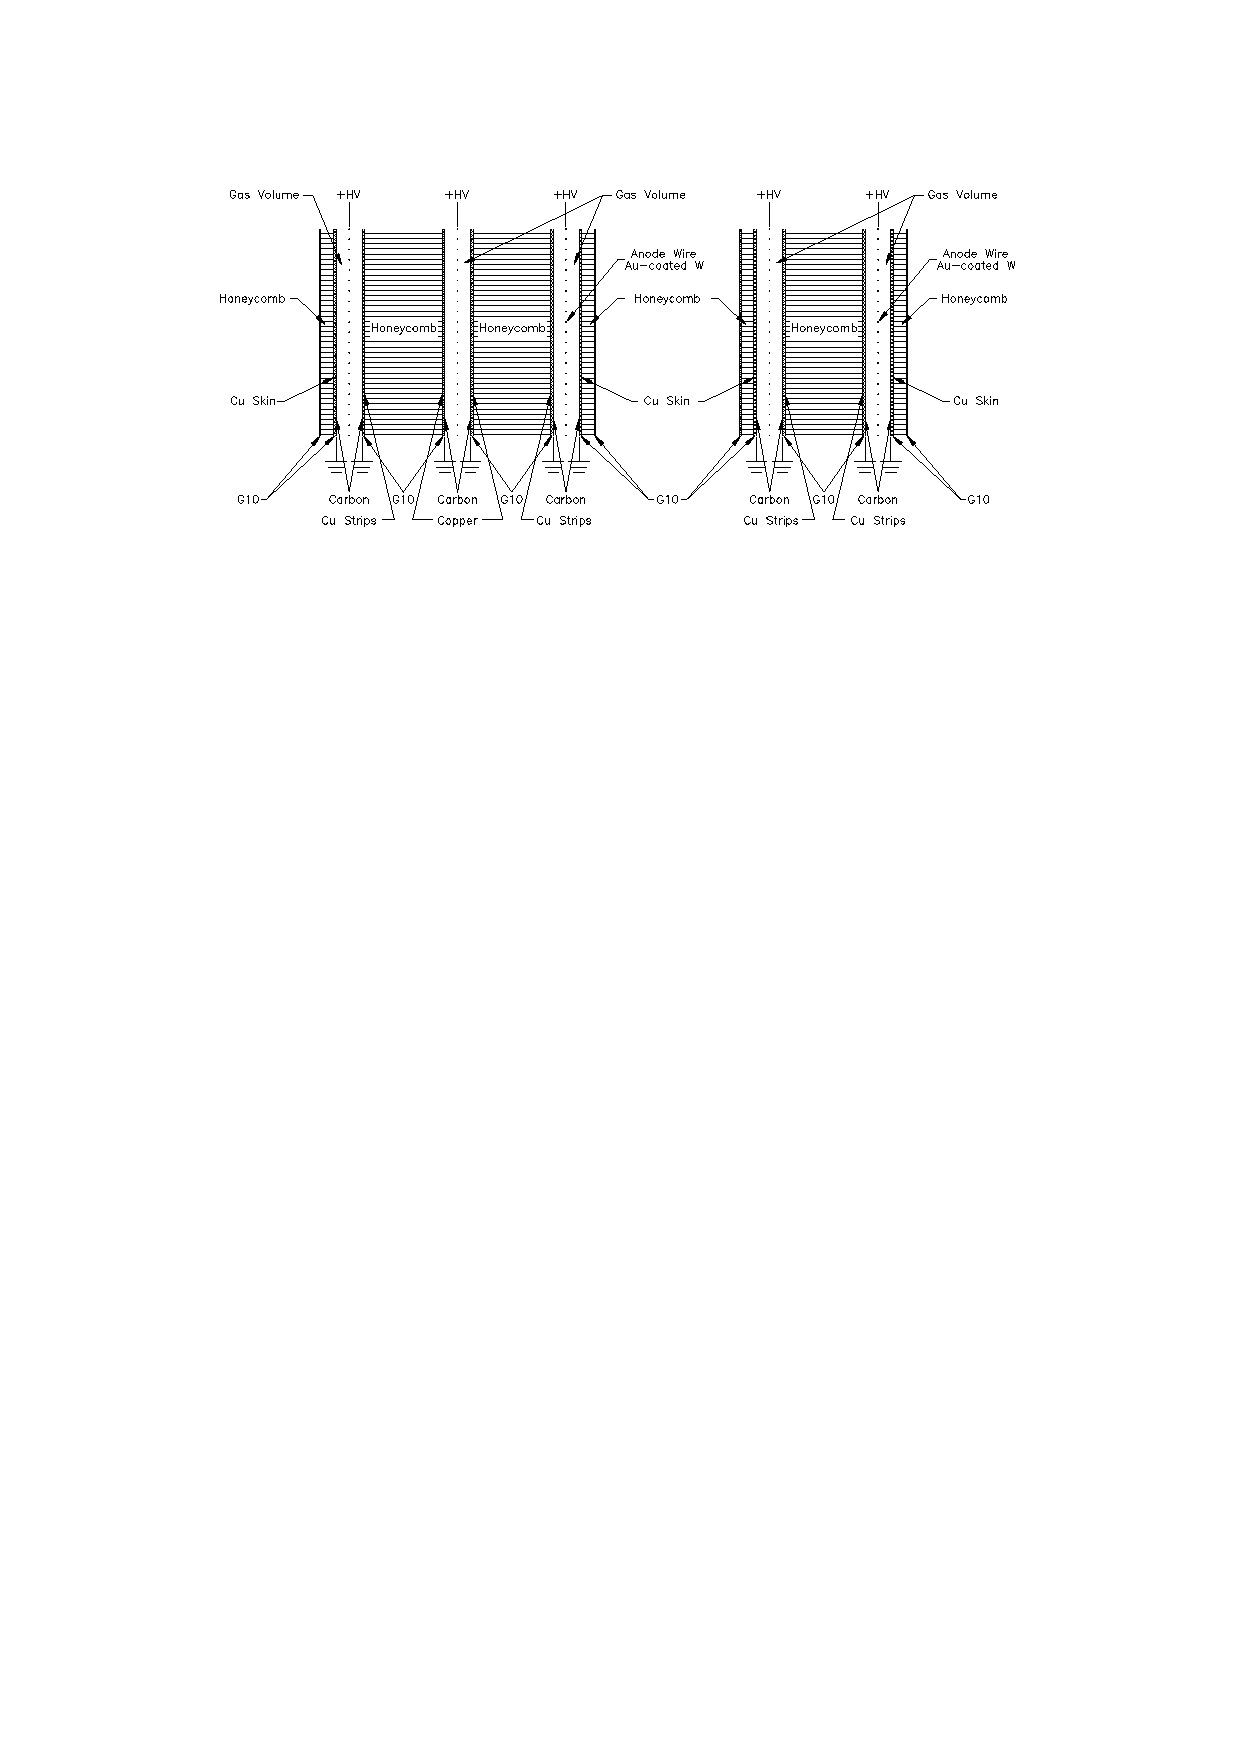
\includegraphics[height=5cm]{fig/Intro/TGC_crosssection.pdf}
\subcaption{TGC DoubletとTripletの断面図}
\end{minipage}%
\caption[TGCチェンバーの断面図]{ (a)はTGCチェンバーの断面図を表す\cite{JINST:2008}。ワイヤーとストリップが直交して張られていることがわかる。 (b)はTGC DoubletとTripletの断面図である。それぞれ2層、3層のガスギャップで構成されており、各ガスギャップの間はペーパーハニカムにより満たされている。}
\label{TGC_structure}
\end{figure}

TGC検出器はトリガー用の検出器であり、ワイヤー間隔が小さいため時間応答がよい。これにより陽子交差頻度である25 nsより細かな時間分解能でミューオンを検出し、そのミューオンがどの陽子バンチ交差に由来するのかを識別 (Bunch Crossing IDentification, BCID) することができる。一方、TGC検出器はそれほど高い位置分解能が求められていないため、ワイヤー電極を4 $\sim$ 20本まとめてから読み出しを行う。結果としてワイヤー、ストリップは合計32万チャンネルをもつ。

図\ref{TGC_picture}にTGC BWの写真を示す。BWの外側の領域 (1.05 < |$\eta$| < 1.92) はエンドキャップ領域、内側の領域  (1.92 < |$\eta$|< 2.4) はフォワード領域と呼ばれ、異なる構造を取っている。エンドキャップ領域では$\phi$方向に48 回対称になるように、フォワード領域では$\phi$方向に24 回対称になるようにチェンバーが設置されている。エンドキャップ領域の 1/48、フォワード領域の 1/24 はトリガー回路的に独立しており、それぞれが "トリガーセクター" と呼ばれる。
また、電源供給、ガス供給、電気回路制御、読み出しの観点からBWは$\phi$方向に 12 個のセクターに分割されており、これを 1/12 セクターと呼ぶ。
\begin{figure} 
    \centering
    \includegraphics[width=14cm]{fig/Intro/TGC_picture.pdf}
    \caption[TGC検出器]{TGC検出器の正面写真 (M1)\cite{cern_document_server}。TGC検出器は電源供給、ガス供給、電気回路制御、読み出しの観点から$\phi$方向に 12 回対称になっており、赤枠で囲った範囲を 1/12 セクターと呼ぶ。また、TGC検出器は$\eta$方向に2種類の構造をとっており、円盤の外側の領域  (1.05 < |$\eta$| < 1.92) をエンドキャップ領域、円盤の内側の領域  (1.92 < |$\eta$|< 2.4) をフォワード領域と呼ぶ。エンドキャップ領域では$\phi$方向に 48 回対称になるよう、フォワード領域では$\phi$方向に 24回 対称になるようにチェンバーが設置されている。}
    \label{TGC_picture}
\end{figure}



\section{TDAQシステムとPhase\two アップグレード}
\label{sec_TDAQ}
    LHCでは 25 nsの間隔で陽子バンチが衝突するため、衝突で生じたすべてのデータを保存することはできない。限られた読み出し帯域とオフラインの計算リソースを最大限有効活用するためには興味のある衝突事象のみを記録するトリガーが重要となる。またトリガー判定がなされたイベントに対して正しくデータを取得するには、トリガーシステムとデータ取得 (data acquisition、DAQ) システムが連動して機能する必要がある。ATLAS実験では、トリガーとデータ取得をまとめてTrigger and Data Acquisition (TDAQ) システムと呼ぶ。本節ではRun 3 でのTDAQシステムとPhase\two でのTDAQシステムについて説明し、Phase\two アップグレードにおける変更点を述べる。
   
    \subsection{Run 3でのTDAQシステム}
    \label{subsec_run3TDAQ}
    図\ref{Run3_TDAQ}にRun 3におけるTDAQシステムの概要を示す。ATLASのトリガーシステムはLevel-1という初段のハードウェアトリガーと、それに続くHigh Level Trigger (HLT) という後段のソフトウェアトリガーから構成される。

    \begin{figure} 
    \centering
    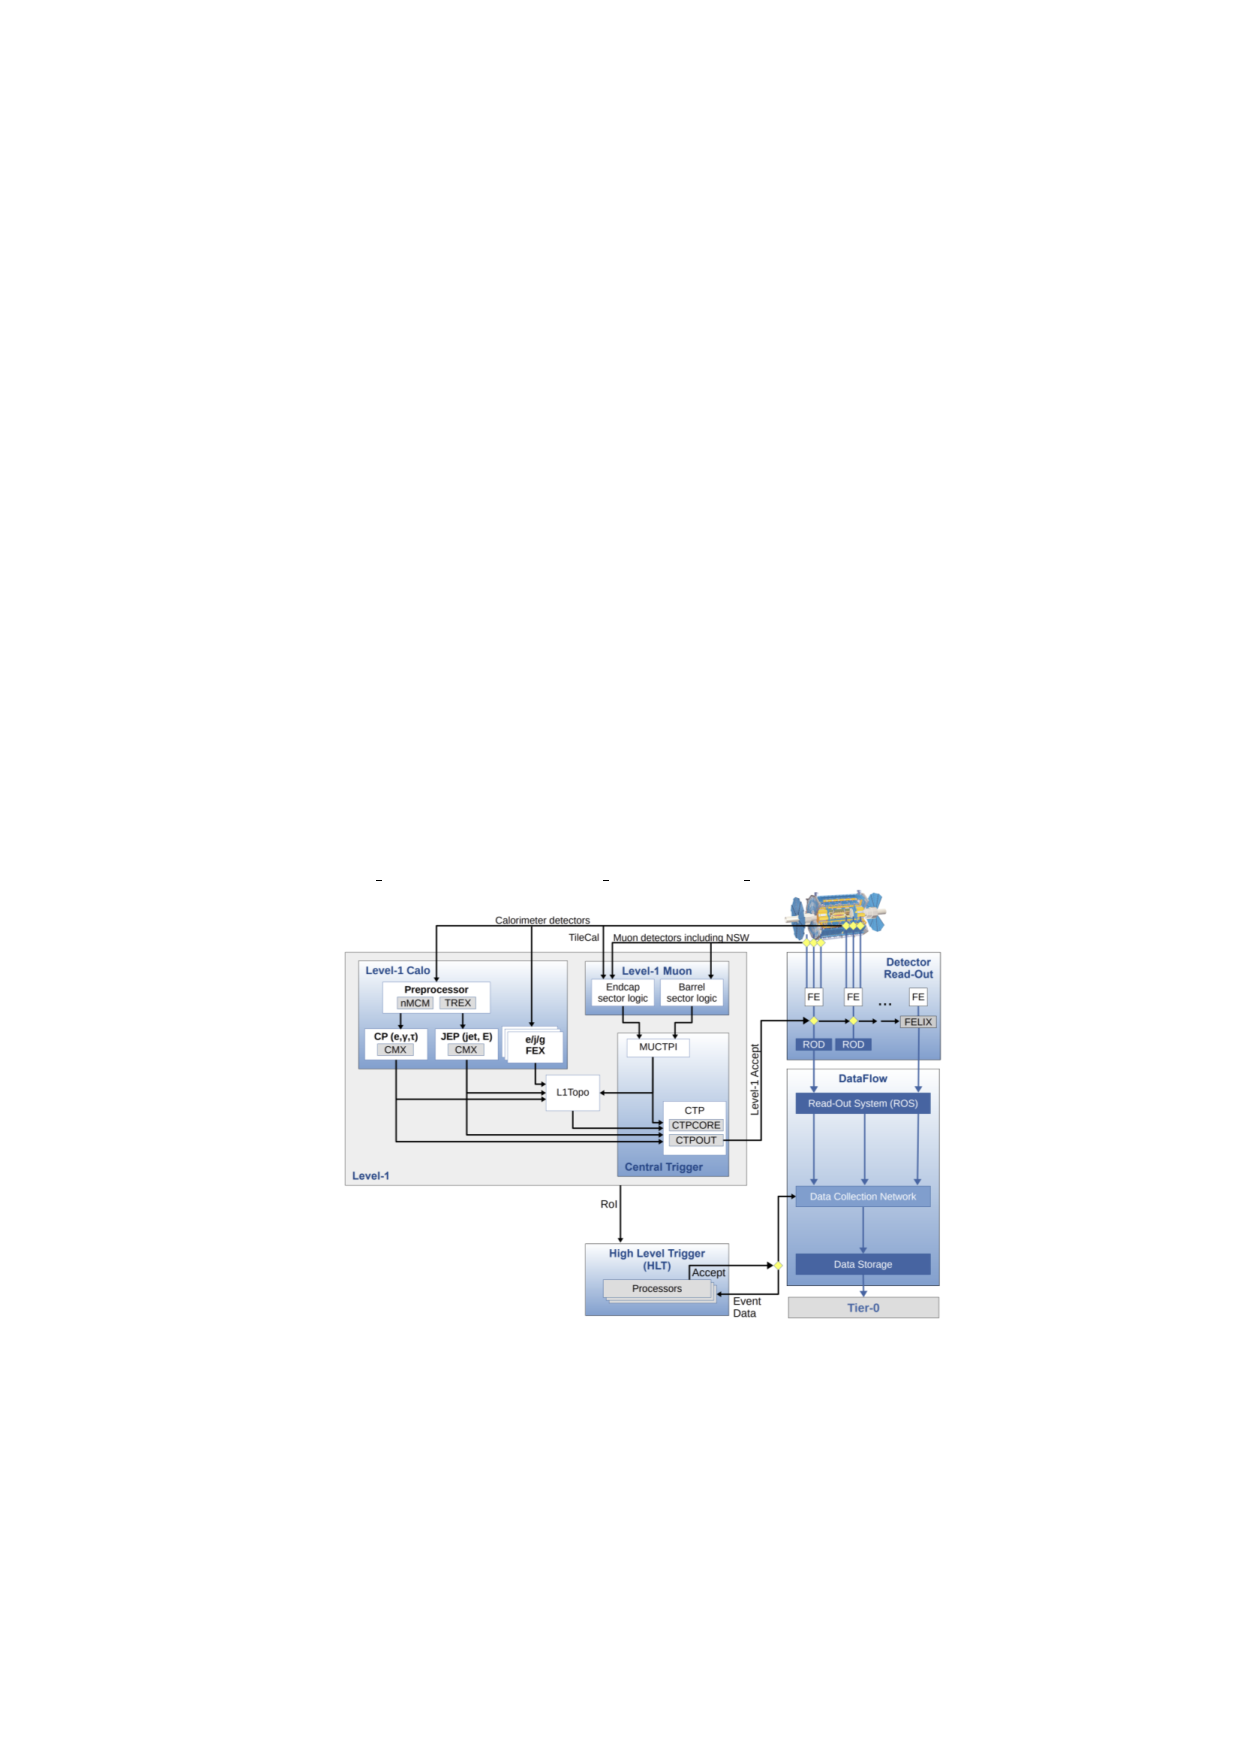
\includegraphics[width=16cm]{fig/Intro/Run3_TDAQ.pdf}
    \caption[Run 3におけるTDAQシステムの概要]{Run 3におけるTDAQシステムの概要\cite{Run3_TDAQ}。トリガーシステムはLevel-1 Triggerという初段のハードウェアトリガーとHigh Level Trigger (HLT)という後段のソフトウェアトリガーから構成される。L1 TriggerはLevel-1 CaloとLevel-1 Muonに大別されCTPで総合的なトリガー判定がなされる。L1 TriggerをパスしたイベントはHLTでより精度の高いトリガー判定が行われ、CERN Permanent Storageに保存される。 }
    \label{Run3_TDAQ}
    \end{figure}

    \subsubsection{Level-1 Trigger}
    \vskip0.5\baselineskip
    Level-1 Triggerは 25 ns間隔で行われるすべての陽子バンチ交差の中から、物理的に興味のある衝突事象を高速で選別する初段トリガーである。L1 Trigger 判定に従い、40 MHzの陽子バンチ交差に対して100 kHzまでのレートでデータが読み出される。L1 Triggerは全ての衝突のデータを処理し、トリガー判定を行う必要があるため、ASICやFPGAなどのハードウェアを利用し、高速処理を実現する。

    ATLASでのL1 Triggerシステムは主にカロリメータートリガー (Level-1 Calo) と ミューオントリガー (Level-1 Muon) で構成される。Level-1 Caloはカロリーメーターからのエネルギー情報をもとに、高いエネルギーを持つ電子、光子、ジェットを検出する。Level-1 MuonはRPCとTGCからの情報をもとに、横方向運動量の大きなミューオンを検出する。RPCとTGCからのトリガー情報はMUon-to Central Trigger Processor Interface (MUCTPI) で統合される。Level-1 CaloとLevel-1 Muonからの信号はCentral Trigger Processor (CTP) に渡され、総合的にLevel-1トリガー判定が行われる。L1 Triggerによって選別されたイベントについては、各検出器のフロントエンド回路にLevel-1 Accept (L1A) が送られ、そのバンチ交差に由来する検出器のヒット信号がReadout Driver (ROD) へと送られる。

    Level-1 Triggerではバンチ交差が生じてからL1Aが届けられるまでの時間 (Level-1 レイテンシー) が一定であるFIxed Latency Schemeを採用している。L1Aが出されるまでの間、陽子バンチ交差で生じるデータは各フロントエンドエレクトロニクス上のバッファーに保管される。現行システムではL1 レイテンシーは2.5 $\mu\mathrm{s}$に設定されており、それを満たすようフロントエンドエレクトロニクスの設計が行われている。

    \subsubsection*{High Level Trigger (HLT) }
    \vskip0.5\baselineskip
    HLTは初段トリガーをパスしたイベントから最終的にストレージに保存する事象を選ぶ役割を担う、ソフトウェアベースのトリガーである。初段トリガーでは使われなかった内部飛跡検出器やMDTなどの精密測定用検出器からの情報も利用して、より高い精度でイベント再構成を行う。HLTによりトリガーレートは3.3 kHzまで削減され、トリガーをパスしたイベントは、データセンターのストレージに記録される。その後CERNのコンピューティングセンターであるTier-0において処理され、イベントが再構成される。

    \subsubsection*{トリガーメニュー}
    ATLAS実験は陽子陽子衝突で生じるさまざまな事象を取得することで、幅広い終状態を持つ多様な物理解析を展開する。広範な物理事象を取得するため、複数のトリガー選別条件が用意されており、それぞれに適切なトリガーレートが分配されている。図\ref{Run2_Triggermenu}にトリガーメニューと呼ばれる、各トリガー選別条件とそれに割り振られたトリガーレートをまとめたリストを示す。
    トリガーメニューでは、解析で利用されるlepton、jet、消失横方向エネルギー ($E_\mathrm{T}^{\mathrm{miss}}$)などの典型的なオブジェクトを取得するための、Level-1およびHLTトリガー閾値が定められている。

    \begin{figure} 
    \centering
    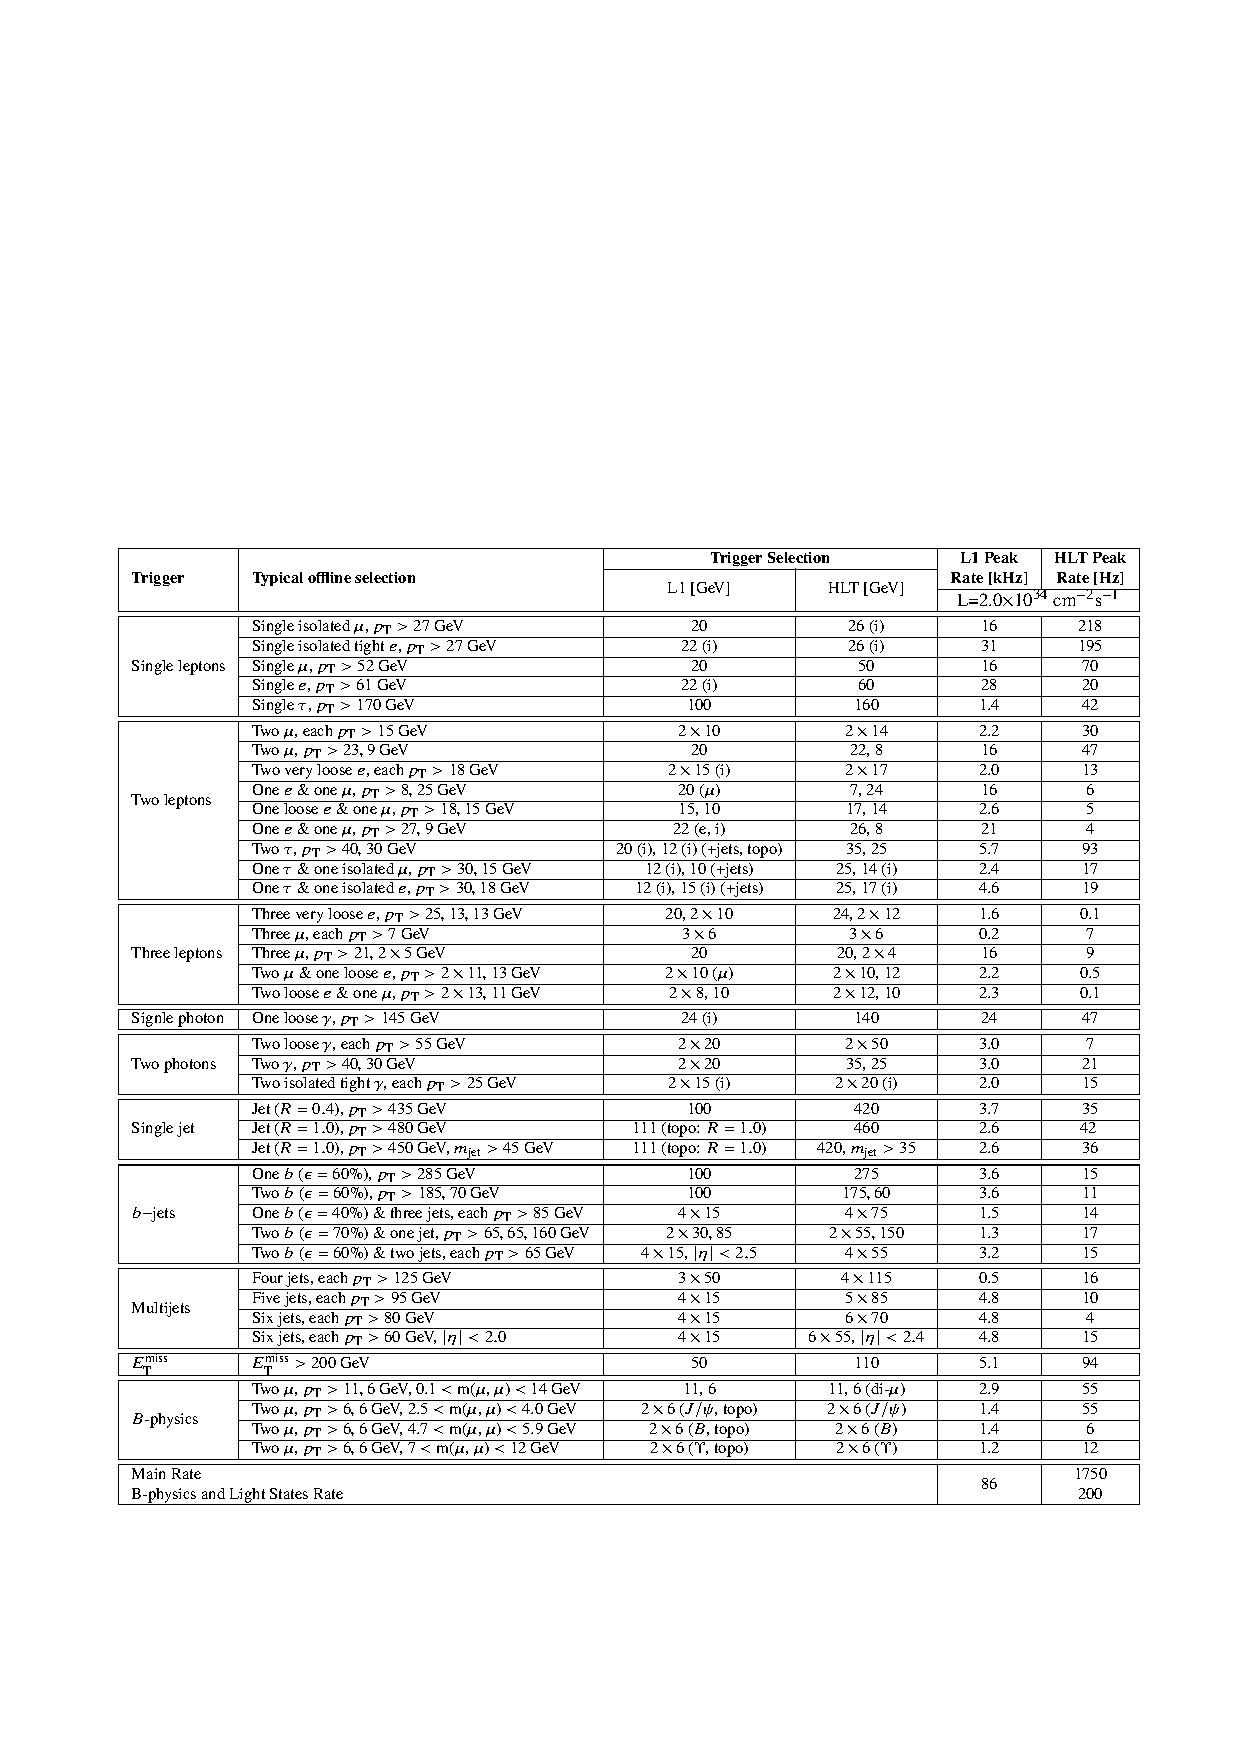
\includegraphics[width=16cm]{fig/Intro/Run2_Triggermenu.pdf}
    \caption[Run2でのトリガーメニューの一例]{Run2でのトリガーメニューの一例\cite{Run2_Triggermenu}。解析で利用される典型的なオブジェクトを取得するためのLevel-1およびHLTでのトリガー閾値が定められる。全体を通してトリガーレートの制約を守るよう設計される。}
    \label{Run2_Triggermenu}
    \end{figure}

    \subsection{高輝度LHC-ATLAS実験でのTDAQシステム}
高輝度LHC-ATLAS実験ではパイルアップによる背景事象が大幅に増加し、トリガーレートが増加する。現行のTDAQシステムのままでは、読み出し能力の限界からトリガー制約を厳しくせざるを得ず、その結果、興味のある物理事象へのアクセプタンスを落としてしまう。そこで高輝度LHC-ATLAS実験に向けて、大規模なTDAQシステムのアップグレードが行われる。初段トリガーレートは 100 kHzから 1 MHzへ、後段トリガーレートは 3.3 kHzから 10 kHzへと拡張される。さらに、初段トリガーレイテンシーも 2.5 $\mu\mathrm{s}$から 10 $\mu\mathrm{s}$へと拡張される。図\ref{Phase2_TDAQ}に高輝度LHC-ATLAS実験でのTDAQシステムの概要を示す。
高輝度LHC-ATLAS実験では初段トリガーをLevel-0 Trigger、後段トリガーをEvent Filter (EF) と呼ぶ。

\begin{figure}
\begin{minipage}[b]{.5\linewidth}
\centering
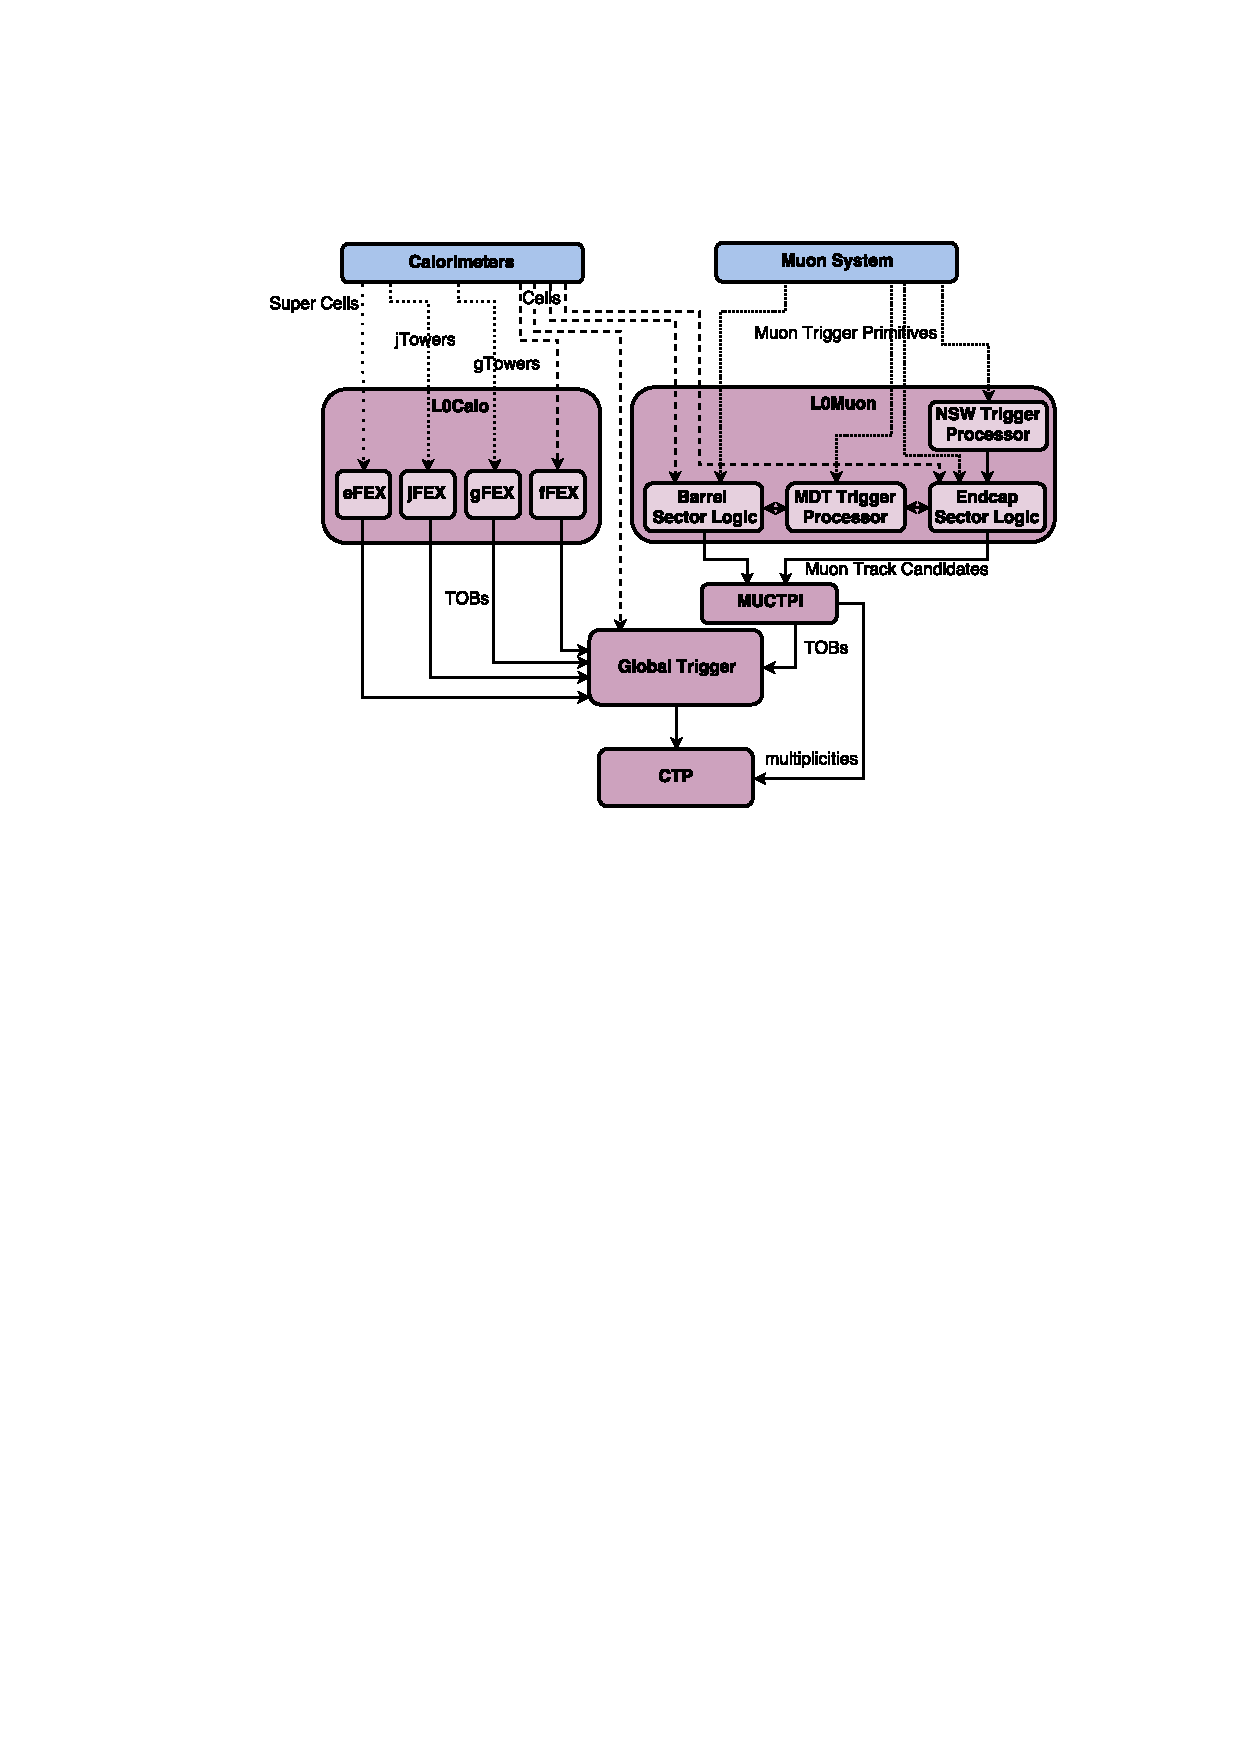
\includegraphics[height=6.5cm]{fig/Intro/Phase2_L0trigger.pdf}
\subcaption{Level-0 Triggerシステムの概要}
\end{minipage}%
\begin{minipage}[b]{.5\linewidth}
\centering
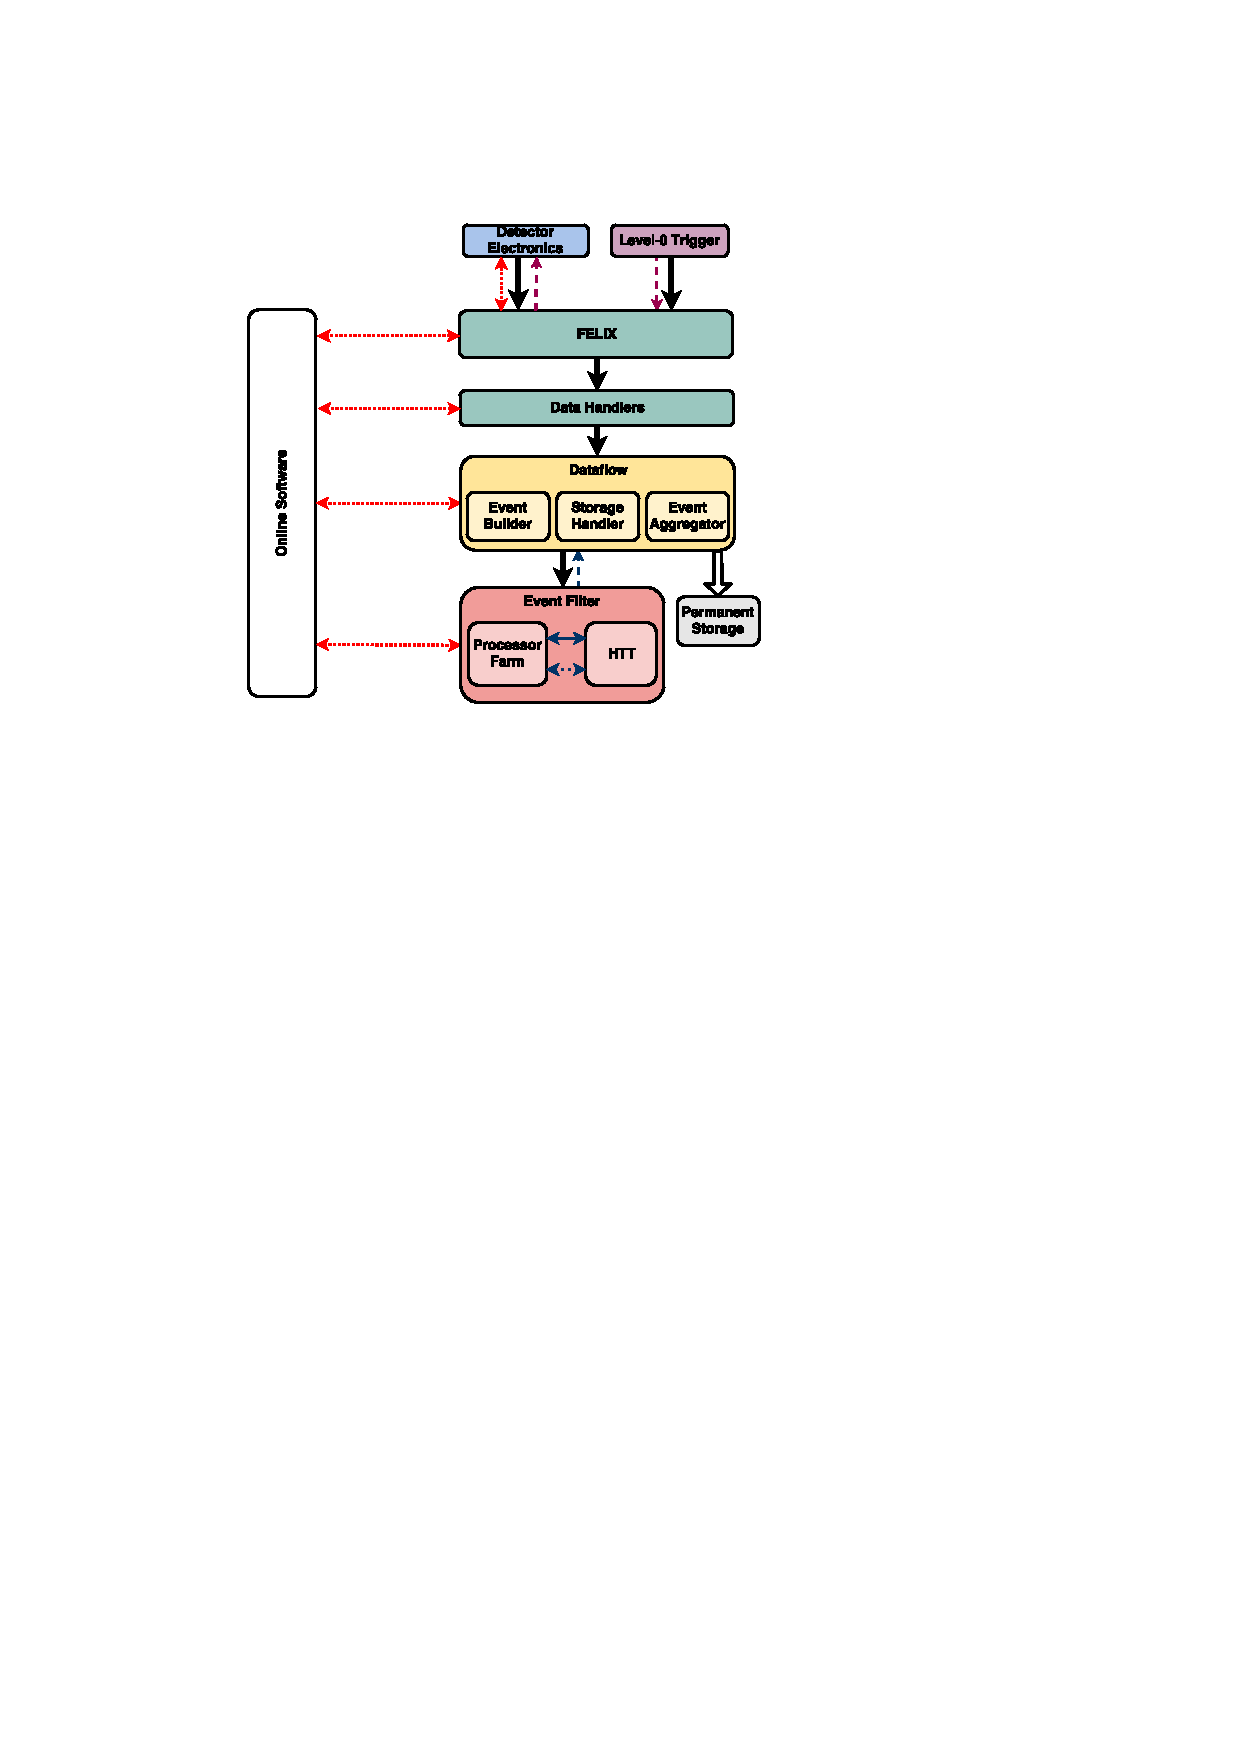
\includegraphics[height=6.5cm]{fig/Intro/Phase2_EF.pdf}
\subcaption{Event FilterとDAQシステムの概要}
\end{minipage}%
\caption[高輝度LHC-ATLAS実験におけるTDAQシステムの概要]{高輝度LHC-ATLAS実験におけるTDAQシステムの概要\cite{tdr_phase2tdaq_2017020}。 (a)にLevel-0 Triggerシステムの概要を示す。Level-0 TriggerはLevel-0 CaloとLevel-0 Muonに大別され、CTPで総合的なトリガー判定がなされる。CTPで後段に送られるべきと判断された場合、FELIXを経由して各フロントエンドエレクトロニクスにL0A信号が分配される。 (b)にEvent FilterとDAQシステムの概要を示す。L0Aを受けた各システムは検出器からのヒットデータをFELIXに送る。FELIXは受け取ったデータをEvent Filterに渡す。EFではソフトウェアベースのトリガー判定が行われ、最後まで残ったデータがCERNのPermanent Strageに保存される。}
\label{Phase2_TDAQ}
\end{figure}

L0 TriggerはL0 Calo、L0 Muon、Global Trigger、CTPで構成される。L0 Muonでは、新たに精密測定用のMDTもトリガーに用いられるようになる。TGCやRPCの情報と組み合わせることで、より精度の高いトリガー判定を実現する。Global TriggerはL0 CaloとMUCTPIからの位置や \pt、\Et などの情報を基に、その事象が特徴的なトポロジーを持つものか判定し、その結果をCTPに送る。CTPはL0 Calo、L0 Muon、L0 Globalからの入力に基づき、トリガーメニュー (図\ref{Phase2_Triggermenu}) に従い、各トリガー条件に指定されたプリスケーリングファクターを適用してトリガー判定を行う。各フロントエンドエレクトロニクスにはFront-End Link eXchange  (FELIX) を経由してLevel-0 Accept (L0A) 信号が分配される。L0Aを受けた各エレクトロニクスは、該当する陽子バンチ交差に由来するデータをFELIXに送信する。FELIXはこれらのデータをEvent Filterに転送する。Event Filterではソフトウェアベースのトリガー判定が行われ、トリガーレートは10 kHzまで削減される。最終的に残った生データは、CERNのデータセンターのストレージに保存される。

\begin{figure} 
\centering
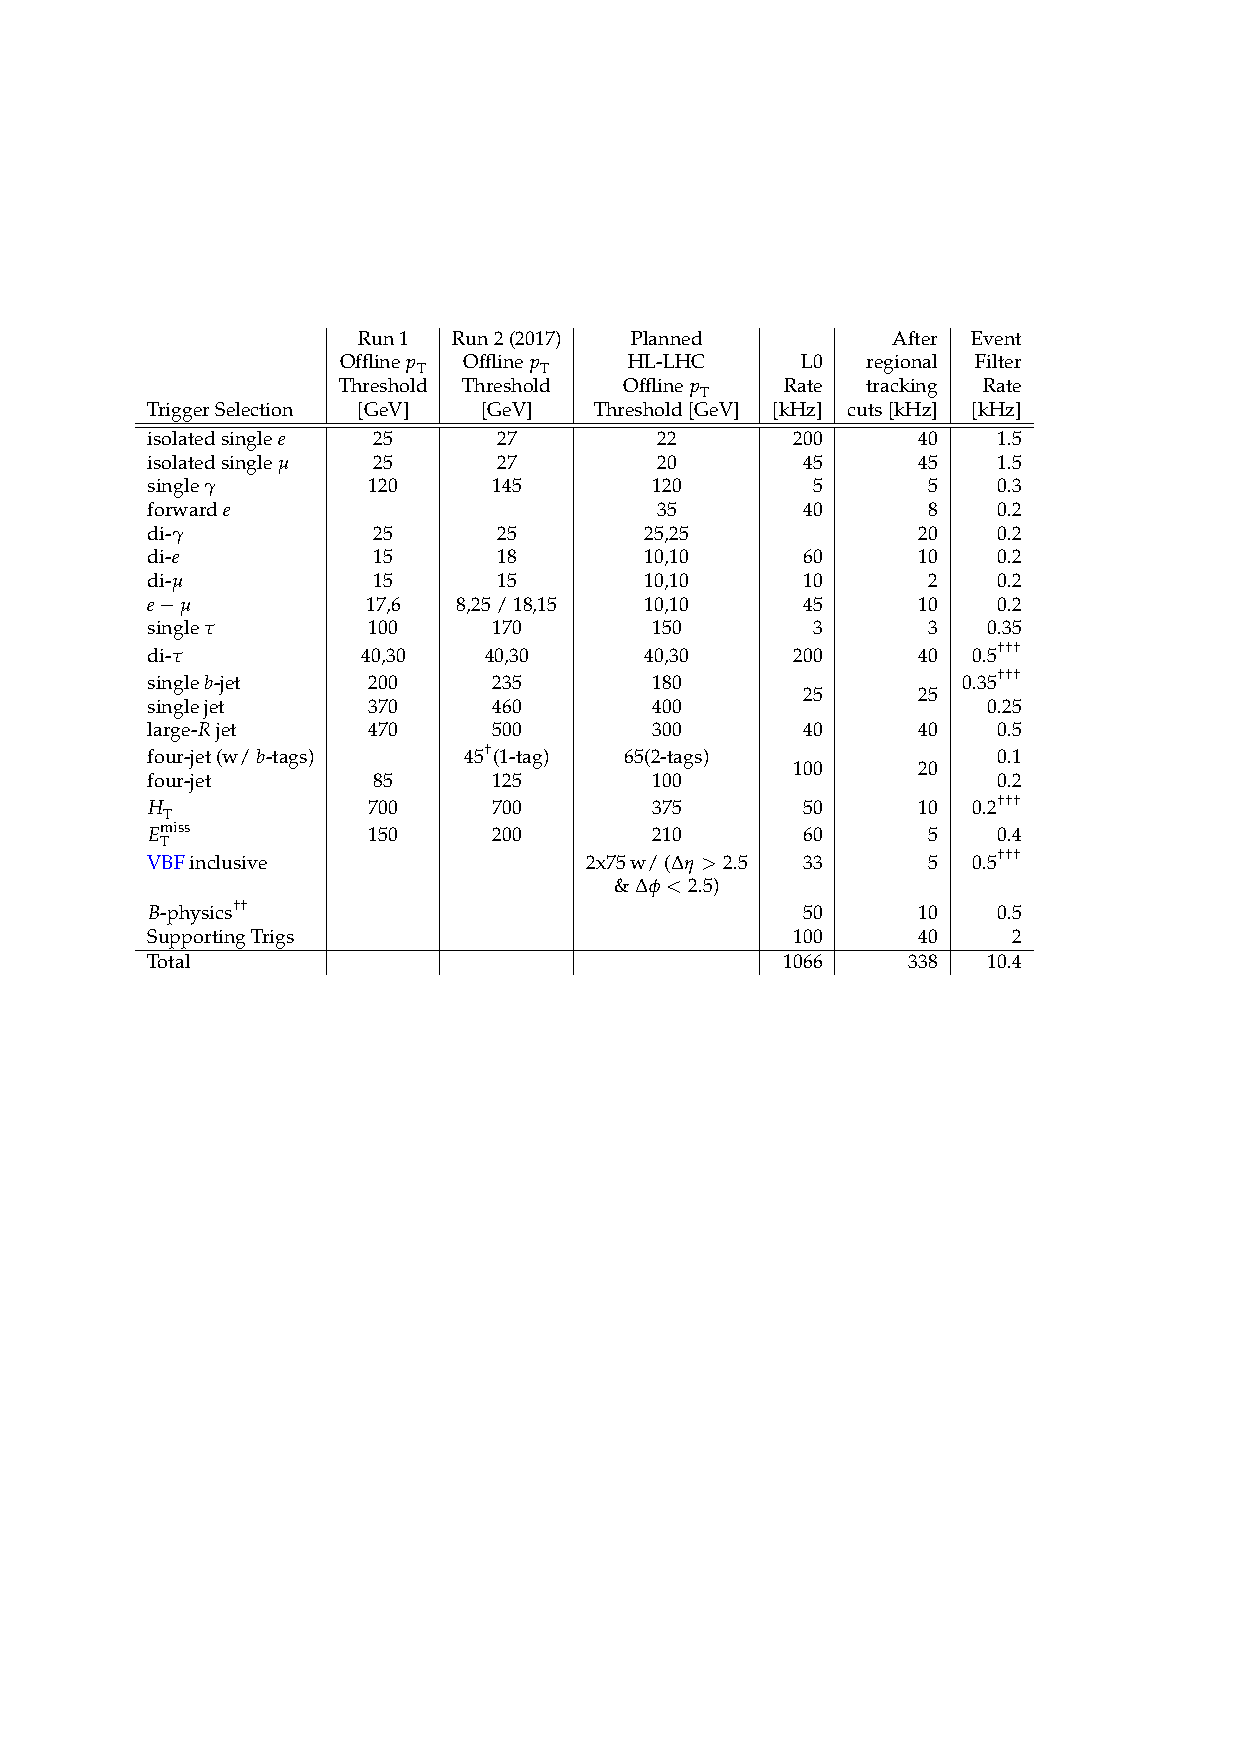
\includegraphics[width=16cm]{fig/Intro/Phase2_Triggermenu.pdf}
\caption[高輝度LHCにおけるトリガーメニューの例]{高輝度LHCにおけるトリガーメニューの例\cite{tdr_phase2tdaq_2017020}。解析に利用される典型的なオブジェクトに対してL0 TriggerおよびEvent Filterでのトリガーレートが分配されている。L0 TriggerレートはRun 3の約10倍、Event Filterでのレートは約6倍に増強される。}
\label{Phase2_Triggermenu}
\end{figure}

\section{TGC検出器の読み出し、トリガー、電気回路システムとPhase\two アップグレード}
\label{sec_TGCtrigger}
高輝度LHC-ATLAS実験に向けたTDAQシステムのアップグレードに伴い、TGC検出器の読み出し、トリガー、電気回路システムも大幅にアップグレードされる。本節ではまず、TGC検出器におけるトリガーのコンセプトを説明する。次にRun 3 でのTGC検出器システムとPhase\two でのTGC検出器システムについて説明し、Phase\two アップグレードにおける変更点を述べる。

    \subsection{TGCトリガーのコンセプト}
    \label{subsec_trigger_concept}
衝突点からエンドキャップ方向  (1.05 < |$\eta$| < 2.4) に飛来するミューオンは、エンドキャップトロイド磁石で曲げられTGC検出器に入射する。TGC検出器の各層ではワイヤー、ストリップによる2次元読み出しで、TGCを通過したミューオンの  ($R$、$\phi$) 座標を検出する。TGC検出器は$z$方向に3つのステーションを持っており、ステーション間のコインシデンスをとることでミューオンの3次元飛跡を再構成し、それをもとに運動量を概算する。より具体的な運動量概算手法の概要を図\ref{TGC_triggerconcept}に示す。

\begin{figure} 
\centering
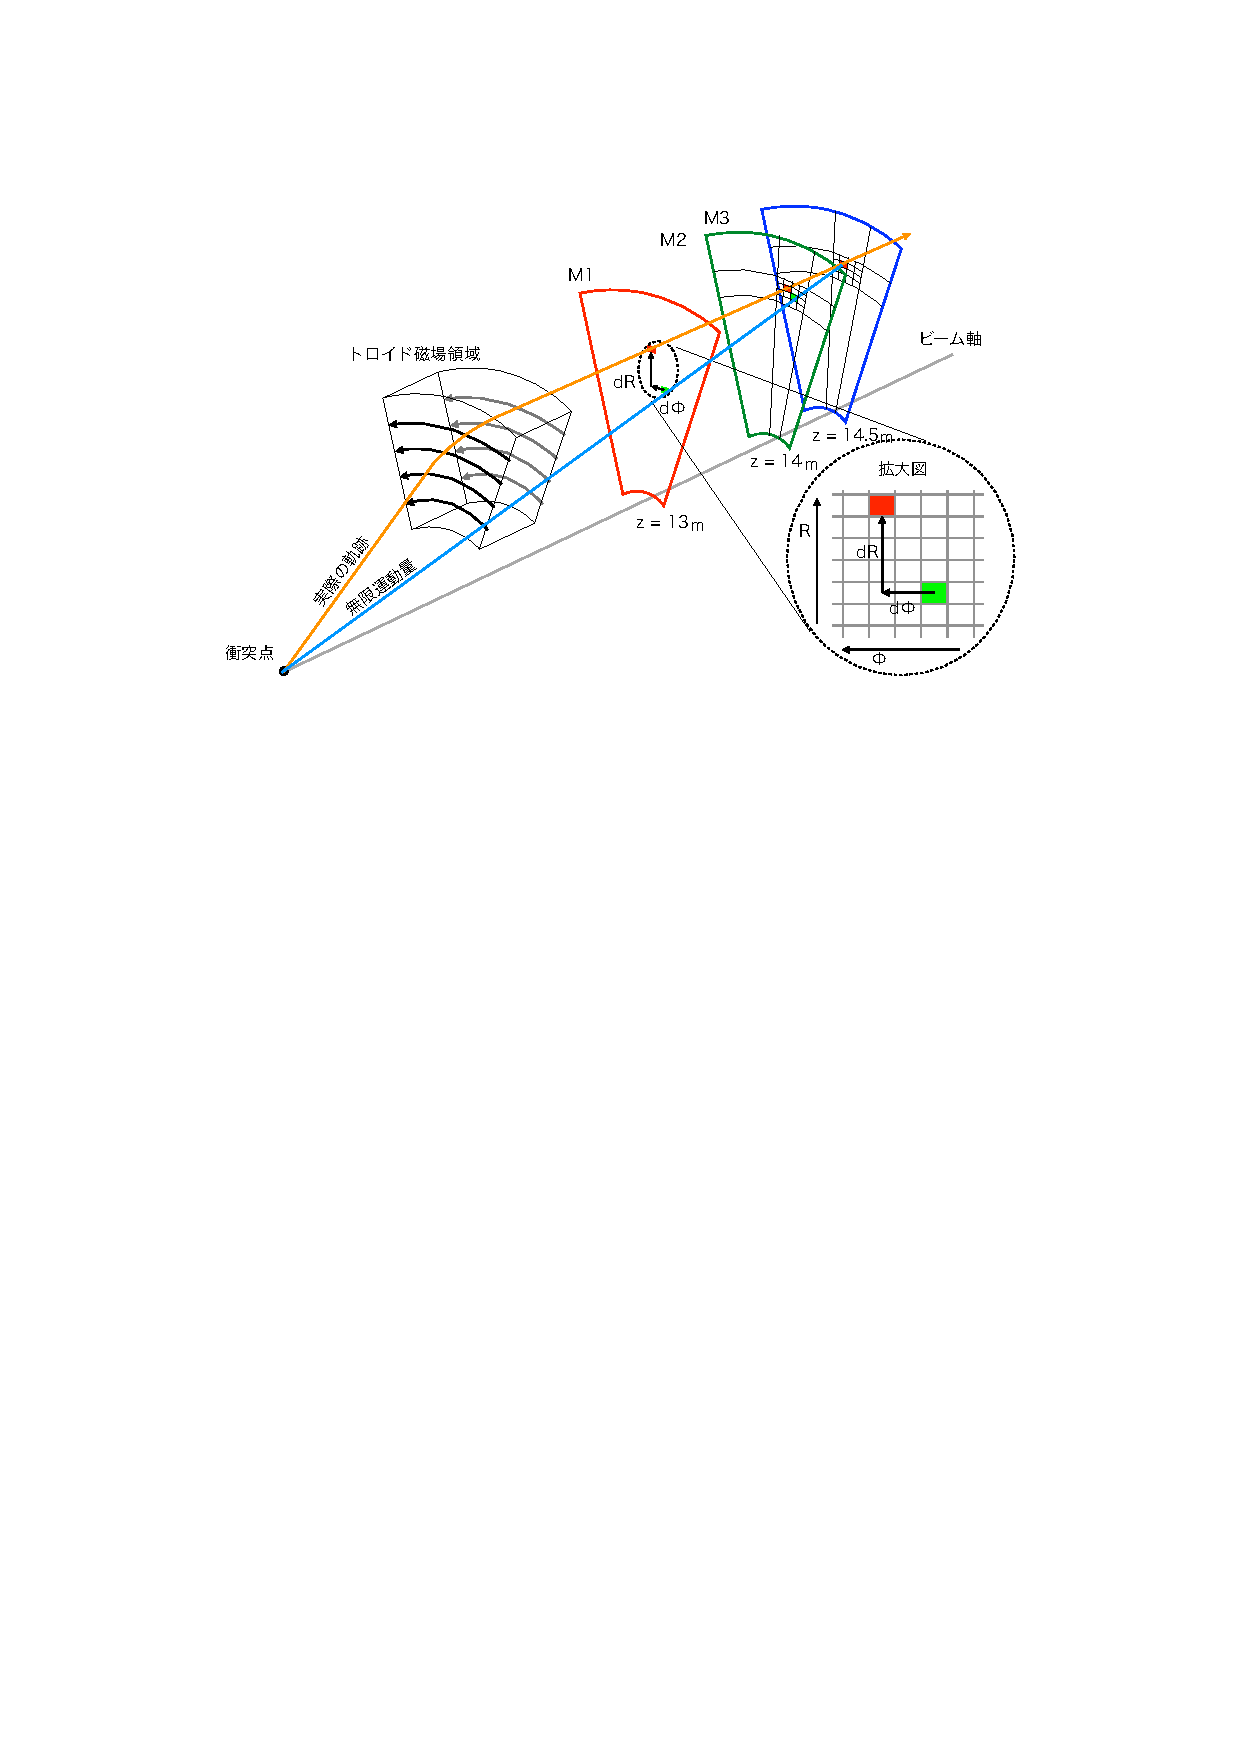
\includegraphics[width=16cm]{fig/Intro/TGC_triggerconcept.pdf}
\caption[TGCにおけるトリガーのコンセプト]{TGCにおけるトリガーのコンセプト\cite{mt_akatsuka}。ミューオンがTGCに残したヒット点から再構成した実際の飛跡と無限運動量飛跡の位置の差分 ($\mathrm{dR}$,$\mathrm{d\phi}$)を利用して\pt を概算する。}
\label{TGC_triggerconcept}
\end{figure}

TGC検出器はエンドキャップトロイド磁場の外側に位置するため、ミューオンは検出器を直線的に通過する。TGC検出器では、3つのステーションのヒットから再構成したミューオンの飛跡 (図中の実際の飛跡) と、M3のヒット点 (ピボット) と衝突点を直線的結んだ無限運動量飛跡のなす角を分別変数に利用して、\pt を概算する。具体的にRun 3のロジックでは、ミューオンが実際に残したヒット点と無限運動量飛跡のM1およびM2の交点との位置の差分  ($\mathrm{d}R$ , $\mathrm{d}\phi$)を 利用する\footnote{高輝度LHC-ATLAS実験では実際の飛跡と無限運動量飛跡のなす角($\mathrm{\Delta\theta, \Delta\phi}$)が利用される。本質的に等価なロジックである。}。特に、ミューオンはエンドキャップトロイド磁場で主に$R$方向に曲げられるため、$\mathrm{d}R$は\pt と強い相関を持った値となる。一方、$\phi$方向にはあまり曲げられないため、衝突点から飛来するミューオンの$\mathrm{d\phi}$は\pt によらず小さい値を取る。そのため$\mathrm{d}\phi$は再構成したミューオン飛跡が、衝突点に由来するものであることを担保する目的で利用される。

\ref{subsec_magnet}節で述べたように、エンドキャップ領域に生成されるトロイド磁場は、$\phi$方向にも$R$方向にも均一ではない上、その大きさも一様でない。そのため、($\mathrm{d}R$ , $\mathrm{d\phi}$)と\pt の関係はミューオンの飛来する場所に依存する複雑な関数となり、代数的にも電気回路的にも求めるのは難しい。そこでシミュレーションを用いて、あらかじめ  ($\mathrm{d}R$ , $\mathrm{d\phi}$) と\pt の関係性をまとめたテーブル  (Look Up Table、LUT) を領域ごとに用意することで、複雑な計算をすることなく、高速で\pt を計算する。この手法をパターンマッチングと呼ぶ。

上述したTGC BW のヒットデータのみを用いたトリガー判定を行なっていたRun 1では、フェイクトリガーと呼ばれる、衝突点に由来しない荷電粒子に対して誤ってトリガーを発行してしまう事象が多く発生していた。図\ref{TGC_faketrigger}にRun 1でのミューオントリガーをパスしたイベント数の$\eta$分布を示す。TGCがトリガーを担当する1.05 < |$\eta$|の領域では、オフラインで再構成されたミューオンイベントよりはるかに多くのイベントがトリガーをパスしていることがわかる。この差分の多くがフェイクトリガーによるものであると考えられる。フェイクトリガーの主な原因として、陽子陽子衝突や、ハドロンカロリメーター内で生じた中性ハドロンが、エンドキャップトロイド磁石の支持構造体と相互作用し、荷電粒子を放出するケースが挙げられる。

この問題に対処するため、Run 2以降のトリガーではInner Coincidenceという新しいロジックが追加された。Inner Coincidenceの概要を図\ref{TGC_Inner_concept}に示す。Inner Coincidenceは、TGC検出器で再構成したミューオン飛跡と、エンドキャップトロイド磁石内部に設置された検出器で再構成したミューオン飛跡のマッチングをとるもので、これによって衝突点に由来する粒子とそうでないものを見分けることが可能となる。さらに、NSWなどの精密測定用の検出器で再構成された飛跡情報を組み合わせることで、TGC BW 単体での\pt 計算より精度を向上させることができる。


\begin{figure} 
\centering
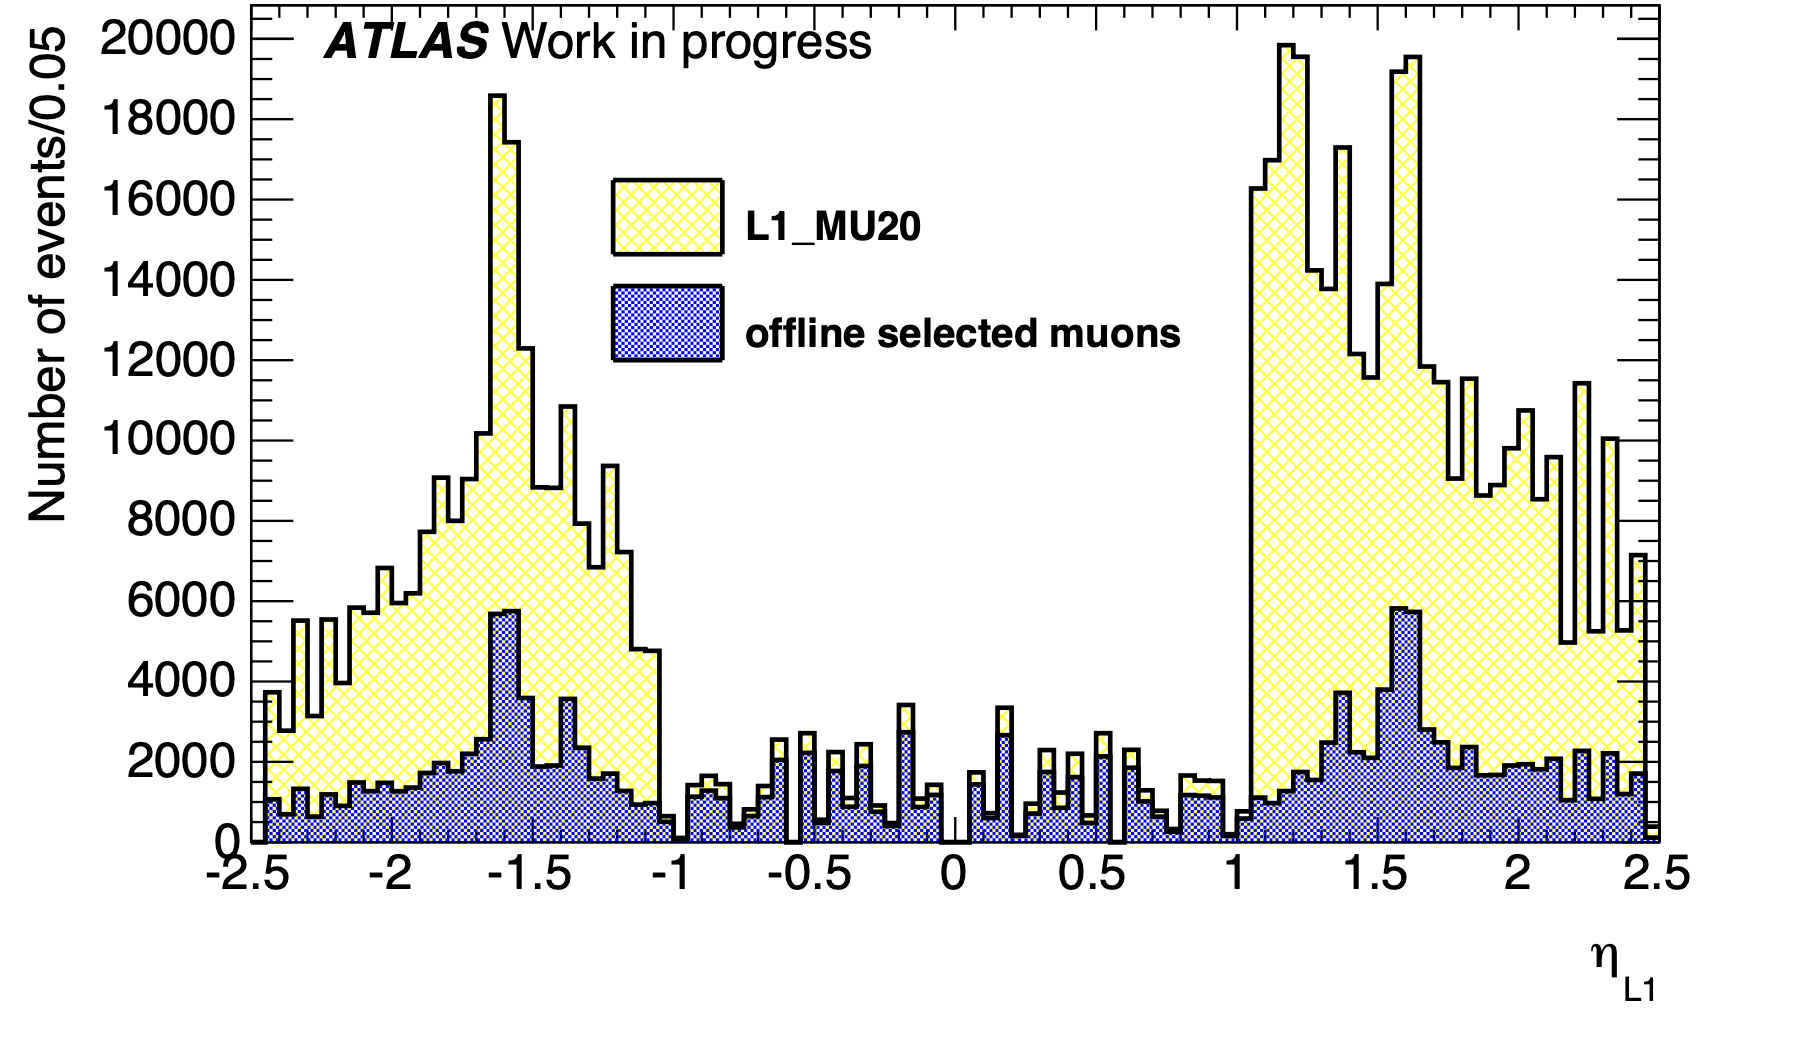
\includegraphics[width=16cm]{fig/Intro/TGC_faketrigger.png}
\caption[Run-1での\pt 閾値]{Run 1における、L1 Muonをパスしたイベント数とオフラインで再構成されたミューオンイベント数の比較。TGCがトリガーを担当する1.05 < |$\eta$|の領域で、オフラインで再構成されたミューオンイベント数より多くのイベントがミューオントリガーをパスしていることがわかる。この差分がフェイクトリガーによるものと考えられる。}
\label{TGC_faketrigger}
\end{figure}

\begin{figure} 
    \centering
    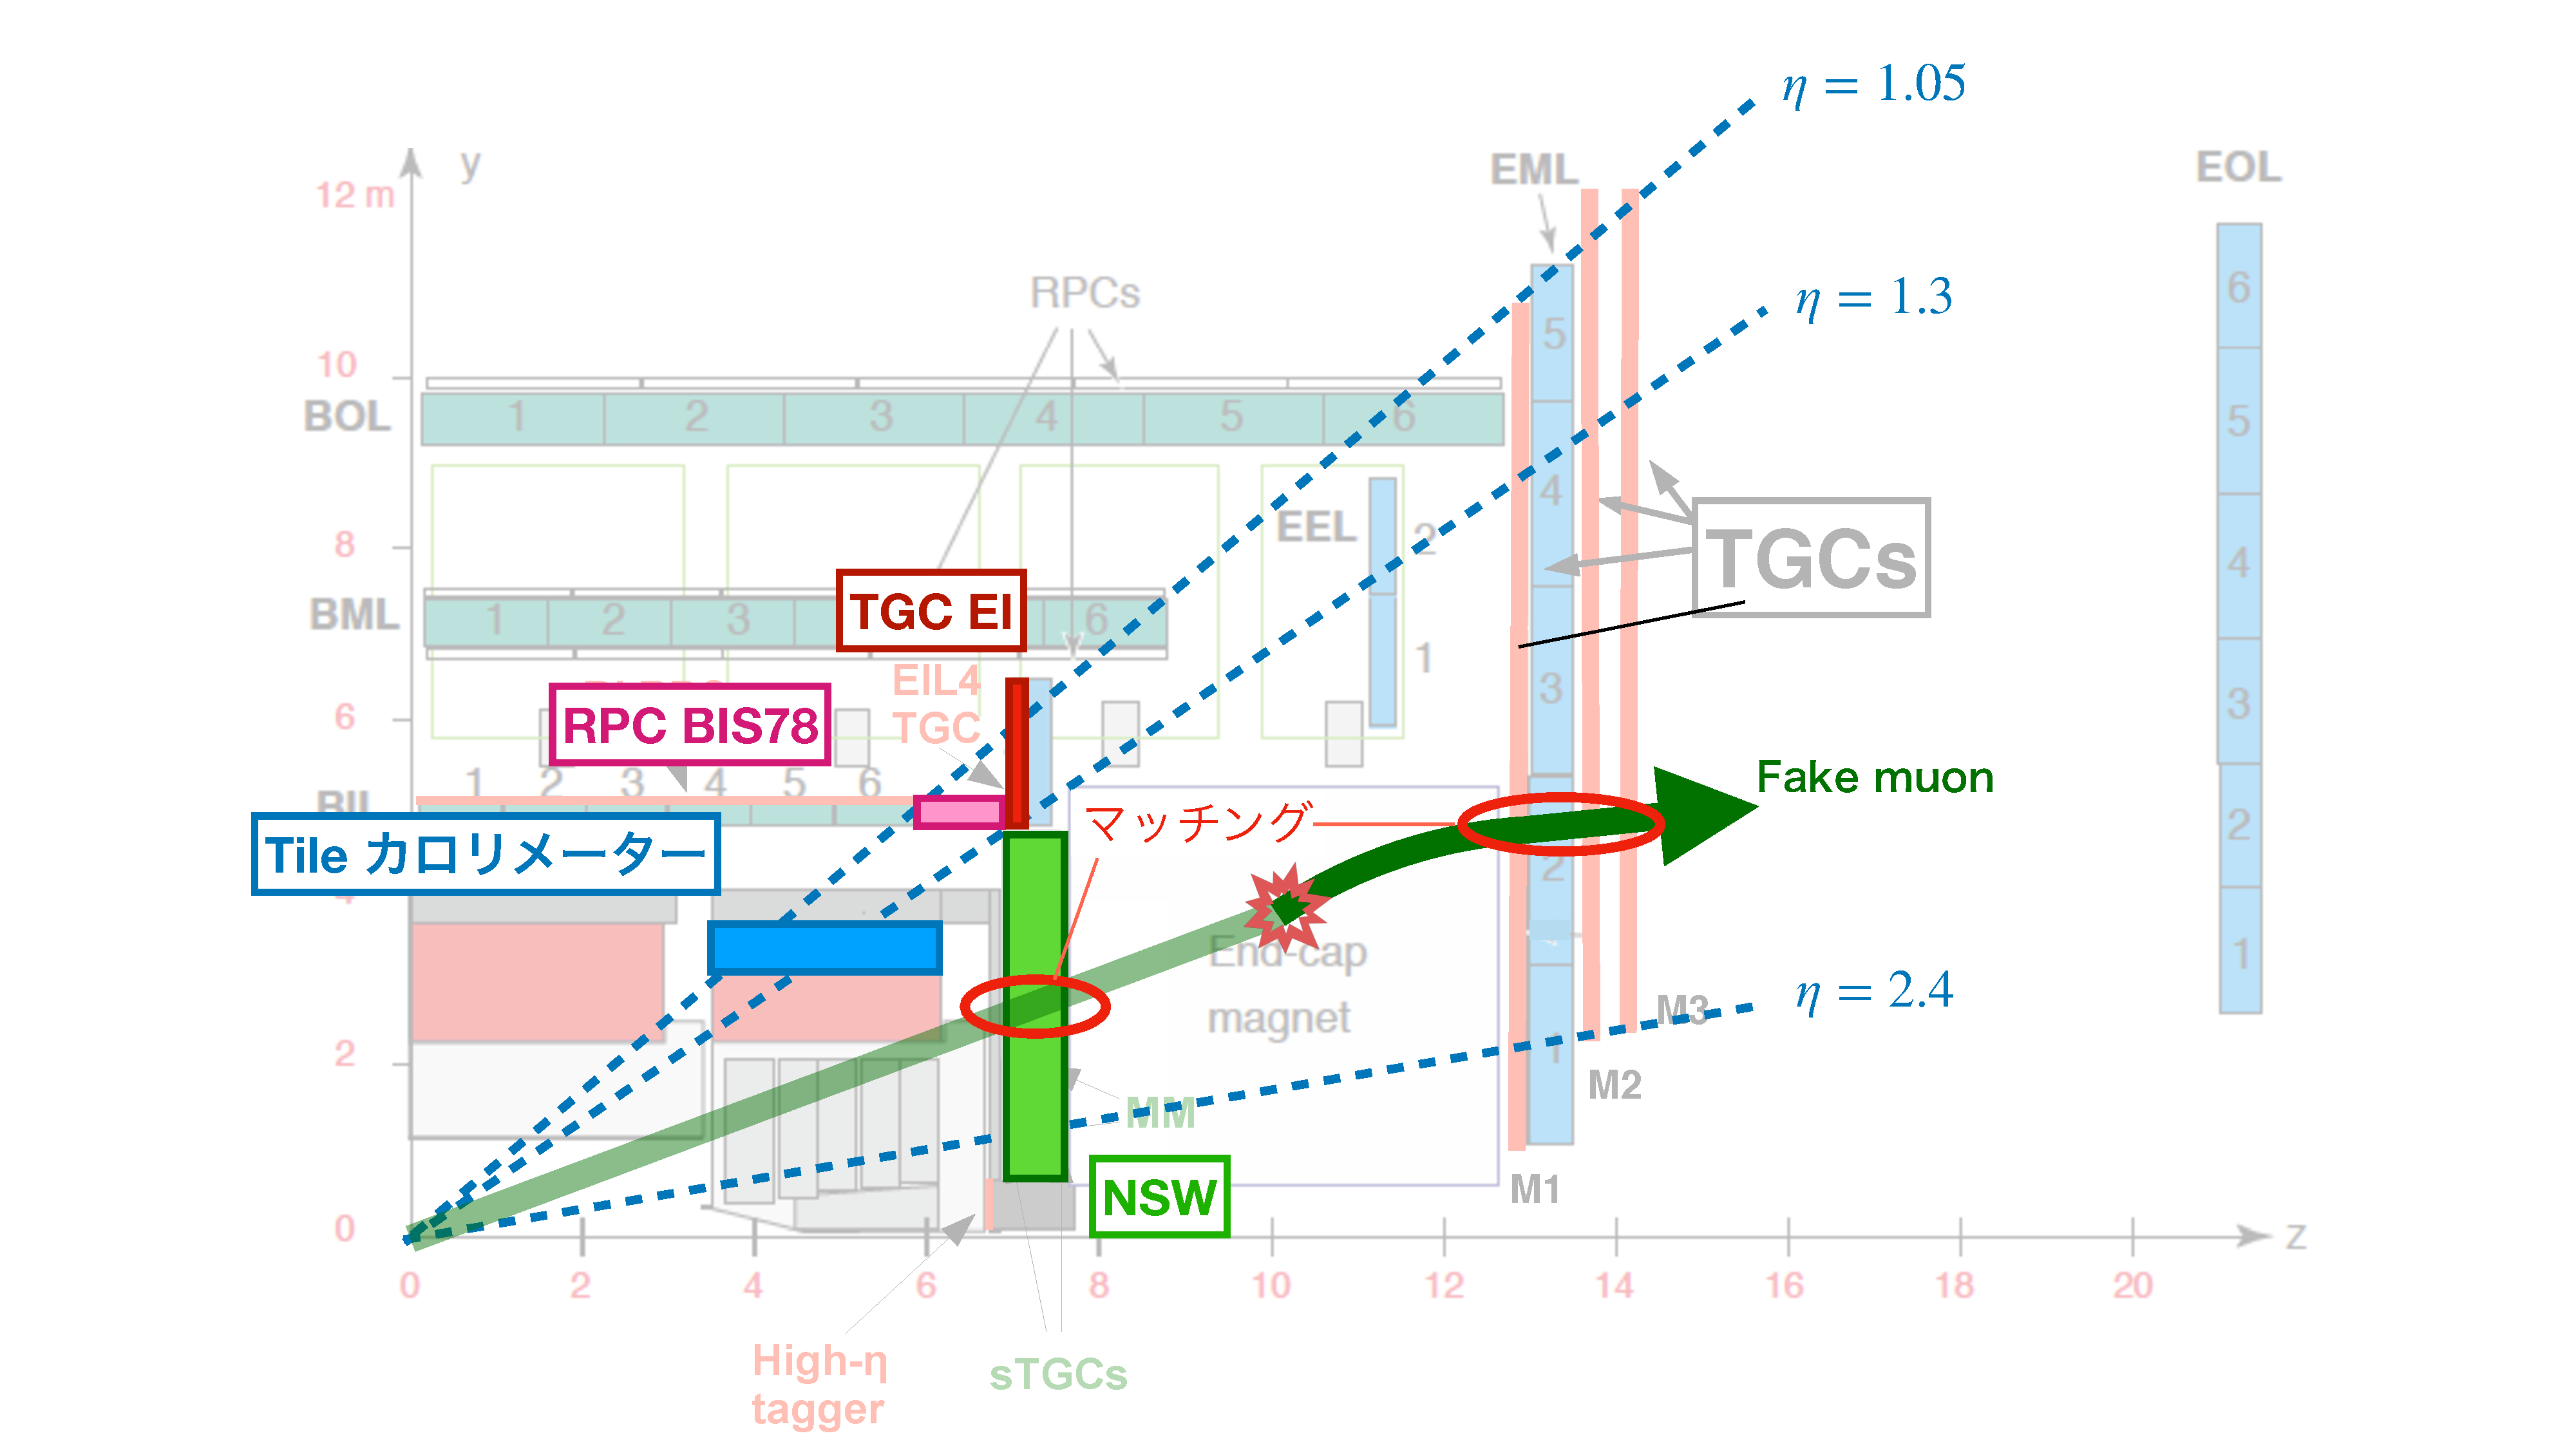
\includegraphics[width=16cm]{fig/Intro/TGC_Inner_concept.pdf}
    \caption[フェイクトリガーの例]{Inner Coincidenceの概念図\cite{mt_kawamoto}。エンドキャップトロイド磁場内部の検出器にヒットを要求することで、衝突点由来でない荷電粒子 (Fake muon) に対してトリガーを発行してしまう事象を削減する。}
    \label{TGC_Inner_concept}
\end{figure}

    \subsection{Run 3でのTGC検出器システム}

\begin{figure} 
\centering
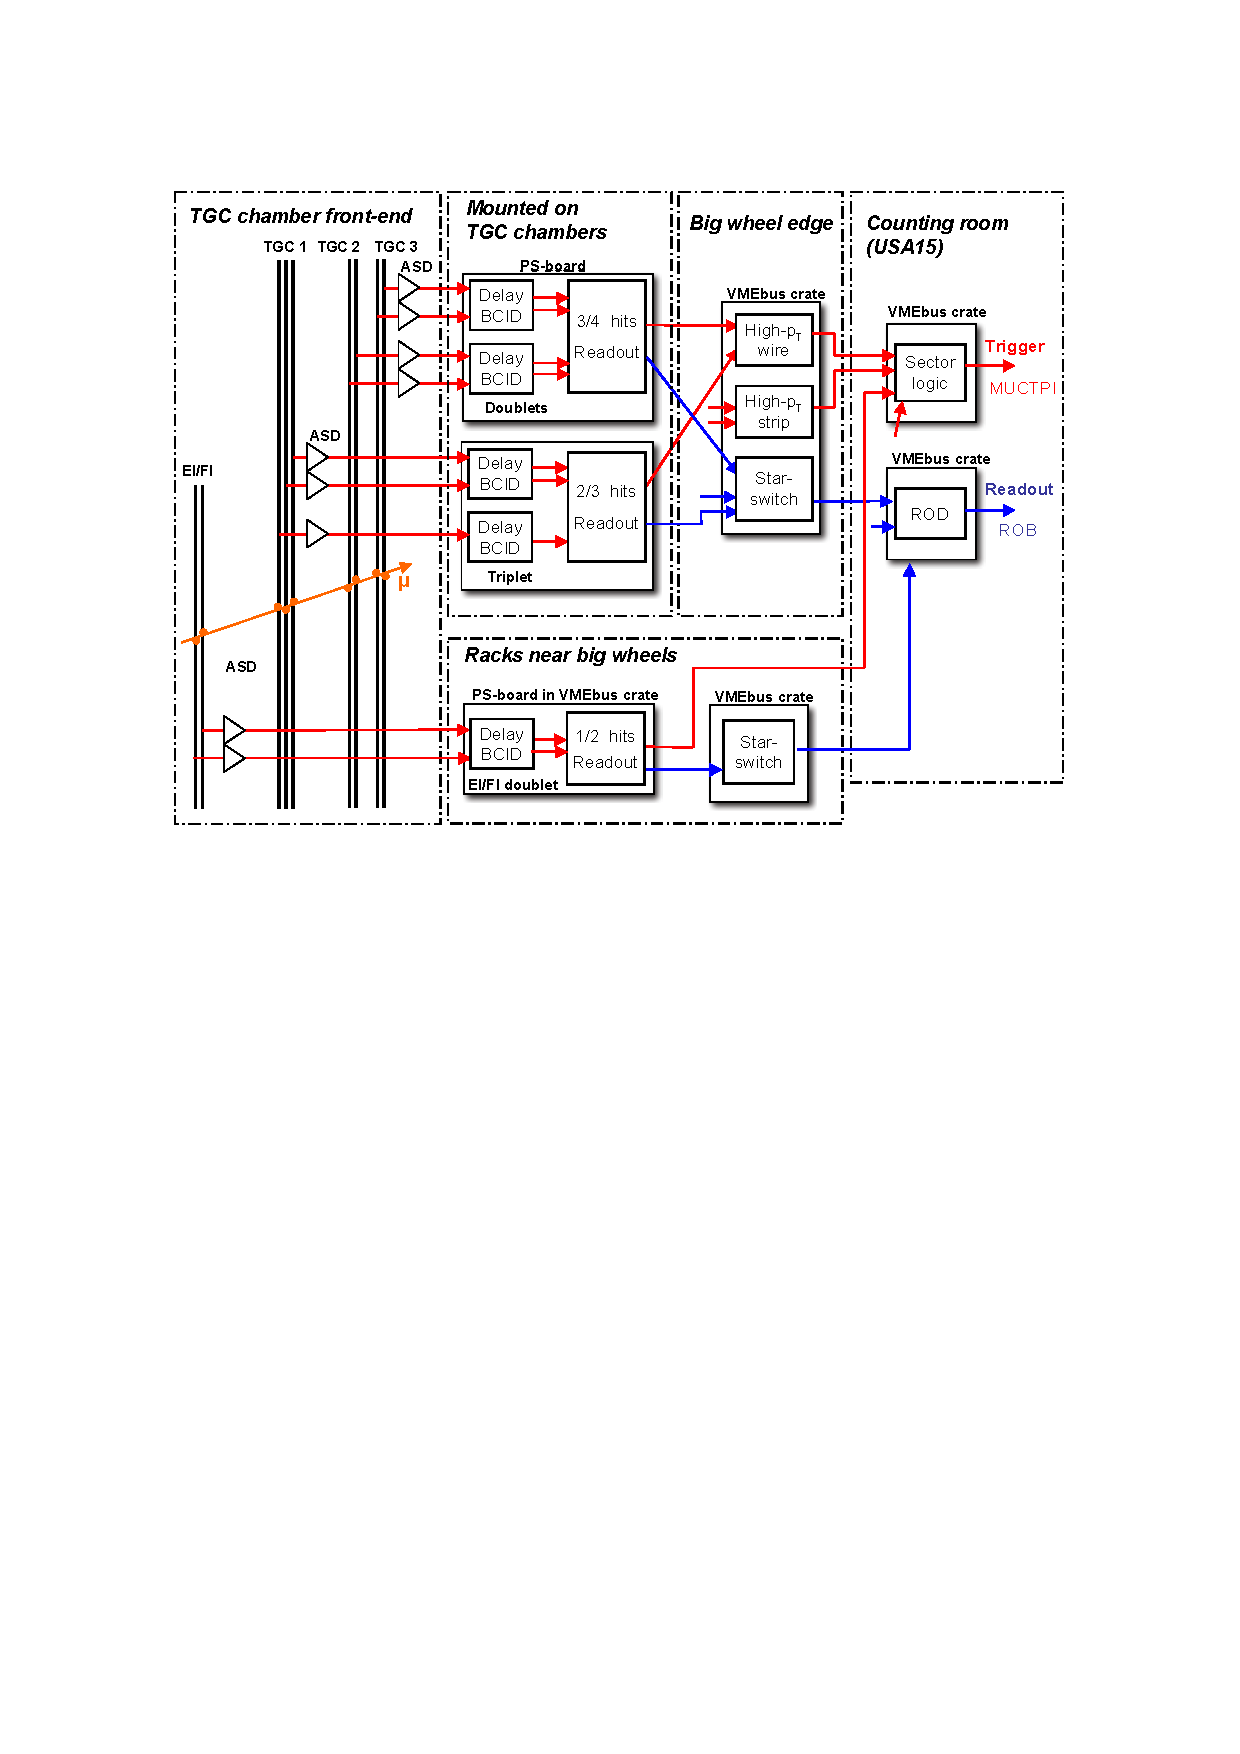
\includegraphics[width=16cm]{fig/Intro/TGC_run3tdaq.pdf}
\caption[Run 3におけるTGC TDAQシステム]{Run 3におけるTGC TDAQシステム。赤線がトリガーパス、青線が読み出しパスを表す。TGC検出器からの電流信号はASDでデジタル信号に変換され、PS boardに集められる。PS boardではBCIDが行われ、ワイヤーとストリップそれぞれでステーション内コインシデンスおよびM2-M3コインシデンスが取られる。その後HPTでM1-M3コインシデンスがとられたのち、SLでワイヤー・ストリップ間コインシデンス及び磁場内部に位置する検出器とのコインシデンスがとられる。SLで得られた$p_\mathrm{T}$情報はMUCTPIを介してCTPに送られ、L1 トリガー判定が行われる。L1 トリガー判定を待っている間、ヒットデータはPS board でバッファーされ、L1A信号が発行された場合にはSSW、RODを通して後段に読み出される。}
\label{TGC_run3tdaq}
\end{figure}

上記のトリガーコンセプトを実現する現行 (Run 3) のTGC TDAQシステムのブロック図を図\ref{TGC_run3tdaq}に示す。図の赤色の線はトリガー判定のための信号の流れを示しており、LHCの陽子バンチ交差に同期してFixed latencyで動作する (トリガーパスと呼ぶ)。青色の線はL1A後のデータ読み出しのための信号の流れを示しており、LHCとは非同期に動作する (読み出しパスと呼ぶ)。TGC検出器にミューオンが入射すると、ガスレイヤーに張られたワイヤーとストリップでアナログの電流信号が発生する。アナログ信号はTGC検出器に直接取り付けられたAmplifier Shaper-Discriminator  (ASD) に集められる。ASDは信号を電圧信号に変換し増幅した後、閾値電圧との比較によりデジタル信号を生成する。デジタル信号は後段のPS board上に搭載されたPatch-Panel ASIC  (PP ASIC) において、どの陽子バンチ交差に由来するものか識別される  (BCID) 。この後から信号はトリガーパスと読み出しパスに分けられる。

トリガーパスは、Slave Board (SLB) ASIC、High-pt (HPT)、Sector Logic (SL) で構成される。SLBではまずワイヤーとストリップ、それぞれでステーション内コインシデンスがとられる。またM2、M3の間のコインシデンスがとられ、($\mathrm{d}R_{23}$,$\mathrm{d\phi_{23}}$)が計算される。その後HPTでM1、M3間のコインシデンスがとられ、($\mathrm{d}R_{13}$,$\mathrm{d\phi_{13}}$)が計算される。SLではM3におけるヒット位置および ($\mathrm{d}R_{13}$,$\mathrm{d\phi_{13}}$)をもとにワイヤー・ストリップ間のコインシデンスがとられ、\pt が概算される。またInner Coincidenceにより、背景事象の除去およびより精度の高い\pt 計算が行われる。SLで再構成された入射位置と\pt 情報は MUCTPI に送られ、CTPへ渡される。CTPでトリガー条件を満たしたバンチ交差にはL1Aが発行される。

読み出しパスはSLB、Star SWitch (SSW)、ReadOut Driver (ROD) というパスを経由して後段へ渡される。PP ASICで同期された信号は、トリガー判定が完了するまでSLB内のL1 Bufferに保存される。SLBでは最大128イベント分の信号をバッファリングすることが可能である。前節で述べた通り、L1 TriggerはFixed latency Schemeを採用しており、L1 Bufferにデータが入ってからそのイベントにL1Aが出されるまでの時間  (L1 latency) は固定されている。そのためSLBはL1Aを受信した後、L1 latencyだけ前のデータを読み出すことで、正しくデータを読み出すことができる。SLBから読み出されたデータはSSWでゼロサプレスと呼ばれるデータ圧縮が行われ、イベント毎にパッケージされる  (Event Building)。RODは1つのセクター内の全てのSLB-SSWから送られたデータ集約し、さらに後段のReadOut System  (ROS) へとデータを送信する。

これらのTGCエレクトロニクスのうち、ASD、PS board、HPT、SSWはATLAS実験室内に設置され、フロントエンドエレクトロニクスと呼ばれる。図\ref{TGC_elec_mount}にフロントエンドエレクトロニクスの設置場所を示す。ASDはTGCチェンバーに直接取り付けられたアダプタボードにマウントされる。PS boardは2枚ごとにアルミニウムで作られたケース  (PS-pack) に収納され、TGCチェンバー付近に設置される。HPTおよびSSWはBWの外側にあるMini-Rack内のVMEクレートに収められる。

SL、ROD以降のエレクトロニクスはUSA15というATLAS回路室内に設置され、バックエンドエレクトロニクスと呼ばれる。HPTとSLおよびSSWとRODはRun 3ではG-linkと呼ばれる旧式の光シリアル通信規格で接続される。G-linkにおけるシリアルデータ転送レートはおよそ800 Mpbsである。

\begin{figure} 
    \centering
    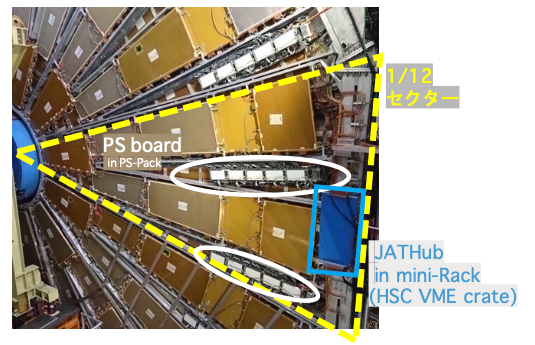
\includegraphics[width=16cm]{fig/Intro/TGC_elec_mount.pdf}
    \caption[TGCエレクトロニクスが設置されている場所]{TGCエレクトロニクスの設置場所。ASDはTGCチェンバーに直接取り付けられたアダプタボードに設置される。PS board は検出器付近のPS-packに収納される。HPT および SSW は BWの外側に設置されたMini-Rack内のVMEクレートに収められる。}
    \label{TGC_elec_mount}
\end{figure}

次にTTC系について述べる。Level1 Bufferより前の読み出し回路およびトリガー回路は、Fixed latency schemeを実現するためLHCの陽子バンチ交差と同期して動作する必要がある。この同期のために、各検出器とLHCを同期させるシステムをTiming, Trigger and Control  (TTC) システムとよび、そのために配布される信号をTTC信号と呼ぶ。TTC信号には陽子バンチ交差と同期した40.079 MHzのLHCバンチ交差クロック  (LHCクロック) やL1A信号などが含まれる。Run 3におけるTTC系の概要を図\ref{Run3_TTC}に示す。TTC信号はCTPから各検出器サブシステムのLocal Trigger Processor  (LTP) に配られる。その後TTC信号はTTCvi、TTCex、TTXrxと呼ばれるTTC専用モジュールおよび専用線を通じて、PS board、HPT、SSW、SLへ分配される。

\begin{figure} 
\centering
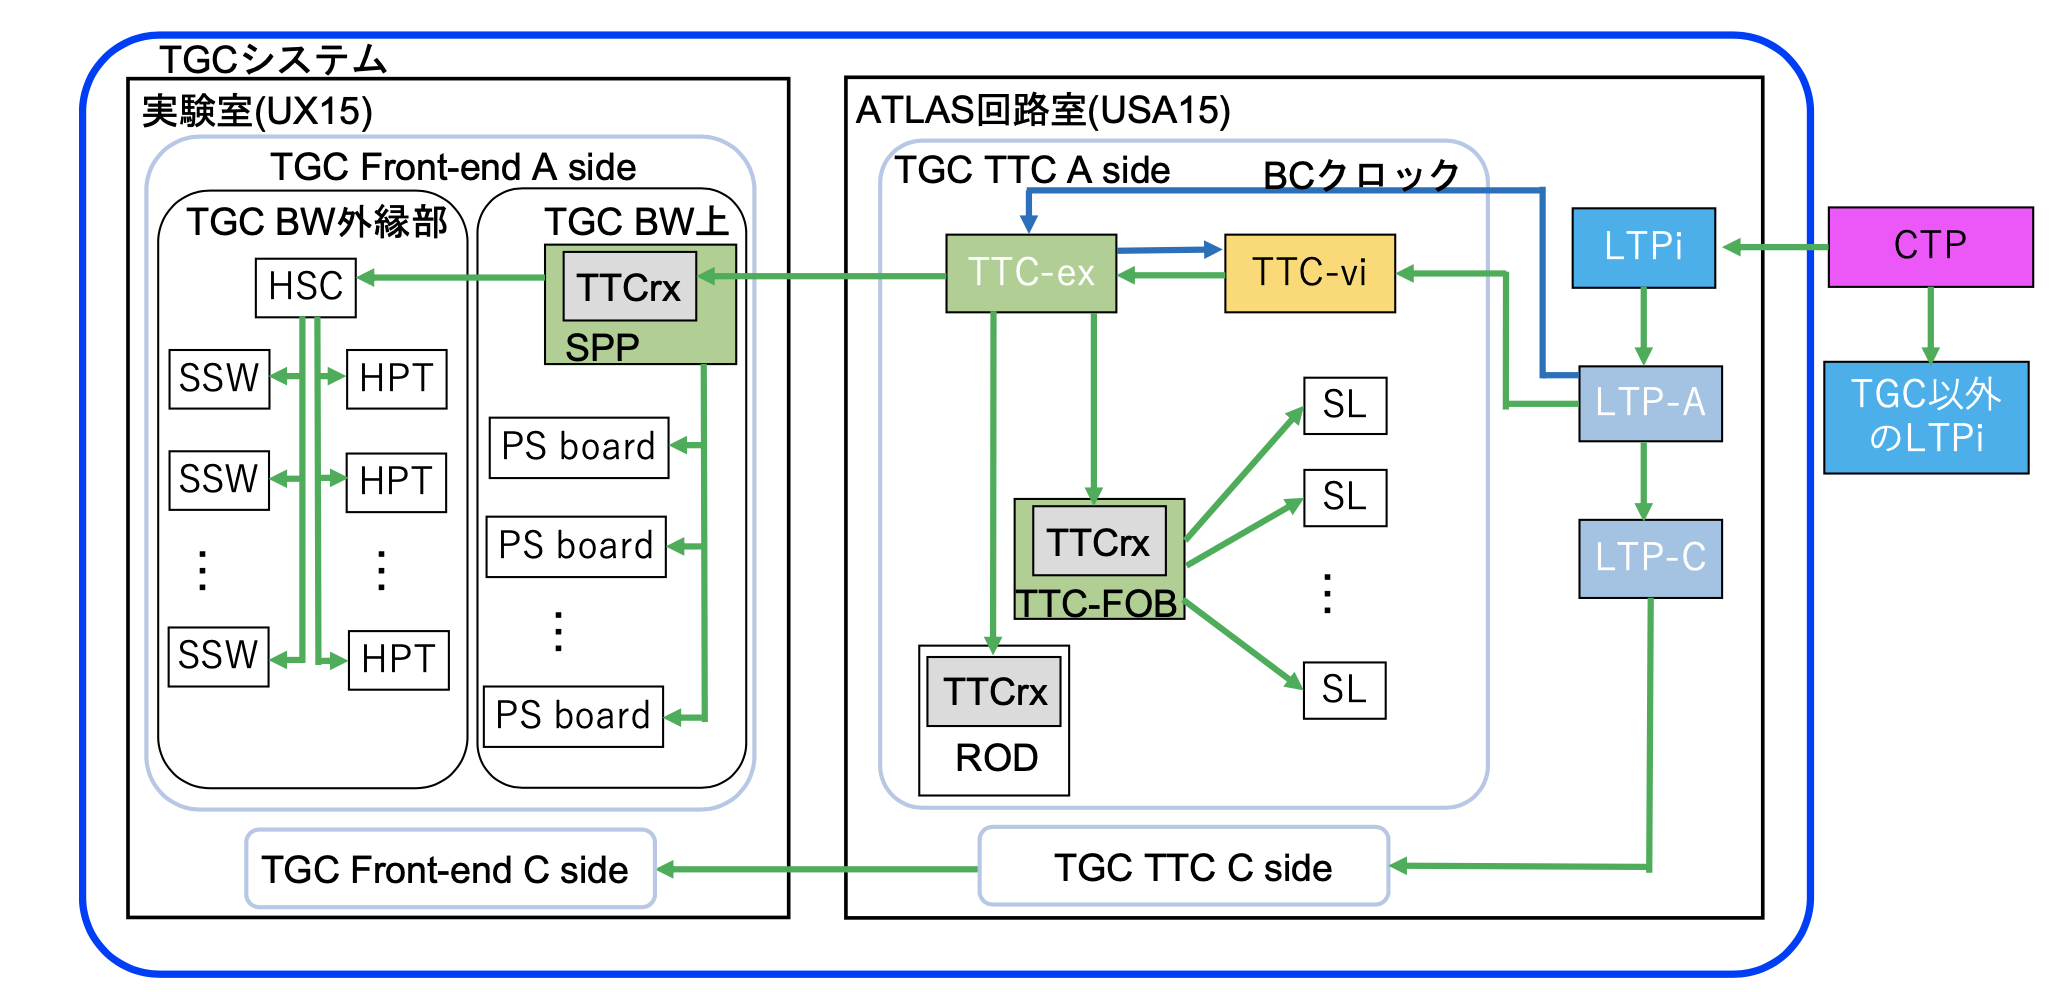
\includegraphics[width=16cm]{fig/Intro/Run3_TTC.png}
\caption[Run 3 TGCシステムにおけるTTCシステムの概要]{Run 3 TGCシステムにおけるTTCシステムの概要\cite{JINST:2008}。TTC信号はCTPから各検出器のサブシステムのLTPに分配され、TTCvi、TTCex、TTCrxを介してPS board、HPT、SSW、SLへと分配される。}
\label{Run3_TTC}
\end{figure}

以上に述べたRun 3のTDAQシステムでは、高輝度LHC-ATLAS実験のトリガーおよび読み出し性能の要求を満たすことができない。この限界は、主にSLBに設置されるL1 Bufferの容量と、ATLAS実験室と回路室間の帯域幅に由来している。Run 3では、L1 Bufferは最大128イベント分のデータしか保存できないため、高輝度LHC-ATLAS実験のL0 latencyの要求である10us (400バンチ) の間データを保持することができない。さらに、1 MHzの初段トリガーレートに対応するデータ量を読み出すためには、現行システムのATLAS実験室と回路室間の帯域幅では不十分である。

    \subsection{高輝度LHC-ATLAS実験でのTGC検出器システム}  
前節で述べた問題を解決するため、高輝度LHC-ATLAS実験ではTGC検出器のエレクトロニクスを大幅にアップグレードする。主な変更点はPS boardでBCIDしたすべてのヒット信号を、ヒットの有無に関わらず、すべてのBCについてSLに送る点である。Run 3のトリガーパスでは、検出器からの信号はSLBやHPTでのコインシデンスを通じて、段階的にデータ量を削減しながら回路室へ送られた。一方、高輝度LHC-ATLAS実験では、実験室と回路室の間で新しく高速シリアル通信技術を導入し、帯域幅を大幅に拡張することで、PS boardが処理した全チャンネル分のヒットビットマップをすべて、回路室のSLへ送信することができる。回路室では、ボードサイズや放射線耐性に対する制約が少なく、SLには大規模なFPGAを搭載することができる。その結果、CTPからL0Aが発行されるまでデータを保管しておくL0 Bufferも余裕を持って実装することができ、10 usのL0 latencyに対応することが可能となる。またSLに1つのトリガーセクター内の全てのPS boardからのヒット信号を集約させることで、TGC BW 7層分のヒットデータを利用した、より包括的なトリガーアルゴリズムを実現する。高輝度LHC-ATLAS実験でのトリガーロジックの詳細は\ref{sec_Phase2TriggerLogic}節で説明する。

\subsection*{全体像}
図\ref{TGC_phase2tdaq}に高輝度LHC-ATLAS実験でのTGC検出器エレクトロニクスの概要を示す。ASDは現行システムのものを引き続き使用する。一方で、Run 3で使われていたPS board、SLB、HPT、SLはすべて撤去され、新しくPrimary ProceSsor board  (PS board)、JTAG AssisTance Hub  (JATHub)、Endcap Sector Logic  (SL) が設置される。PS boardはRun 3と同様にPS-packに格納され、TGC検出器付近に設置される。JATHubはMini-pack内のVMEクレートに設置される。SLはUSA15のATCAクレートに設置される。1つのSLはTGCの1/24セクター担当し、このセクターを担当する最大31枚のPS boardからヒットデータを受け取る。

\begin{figure} 
\centering
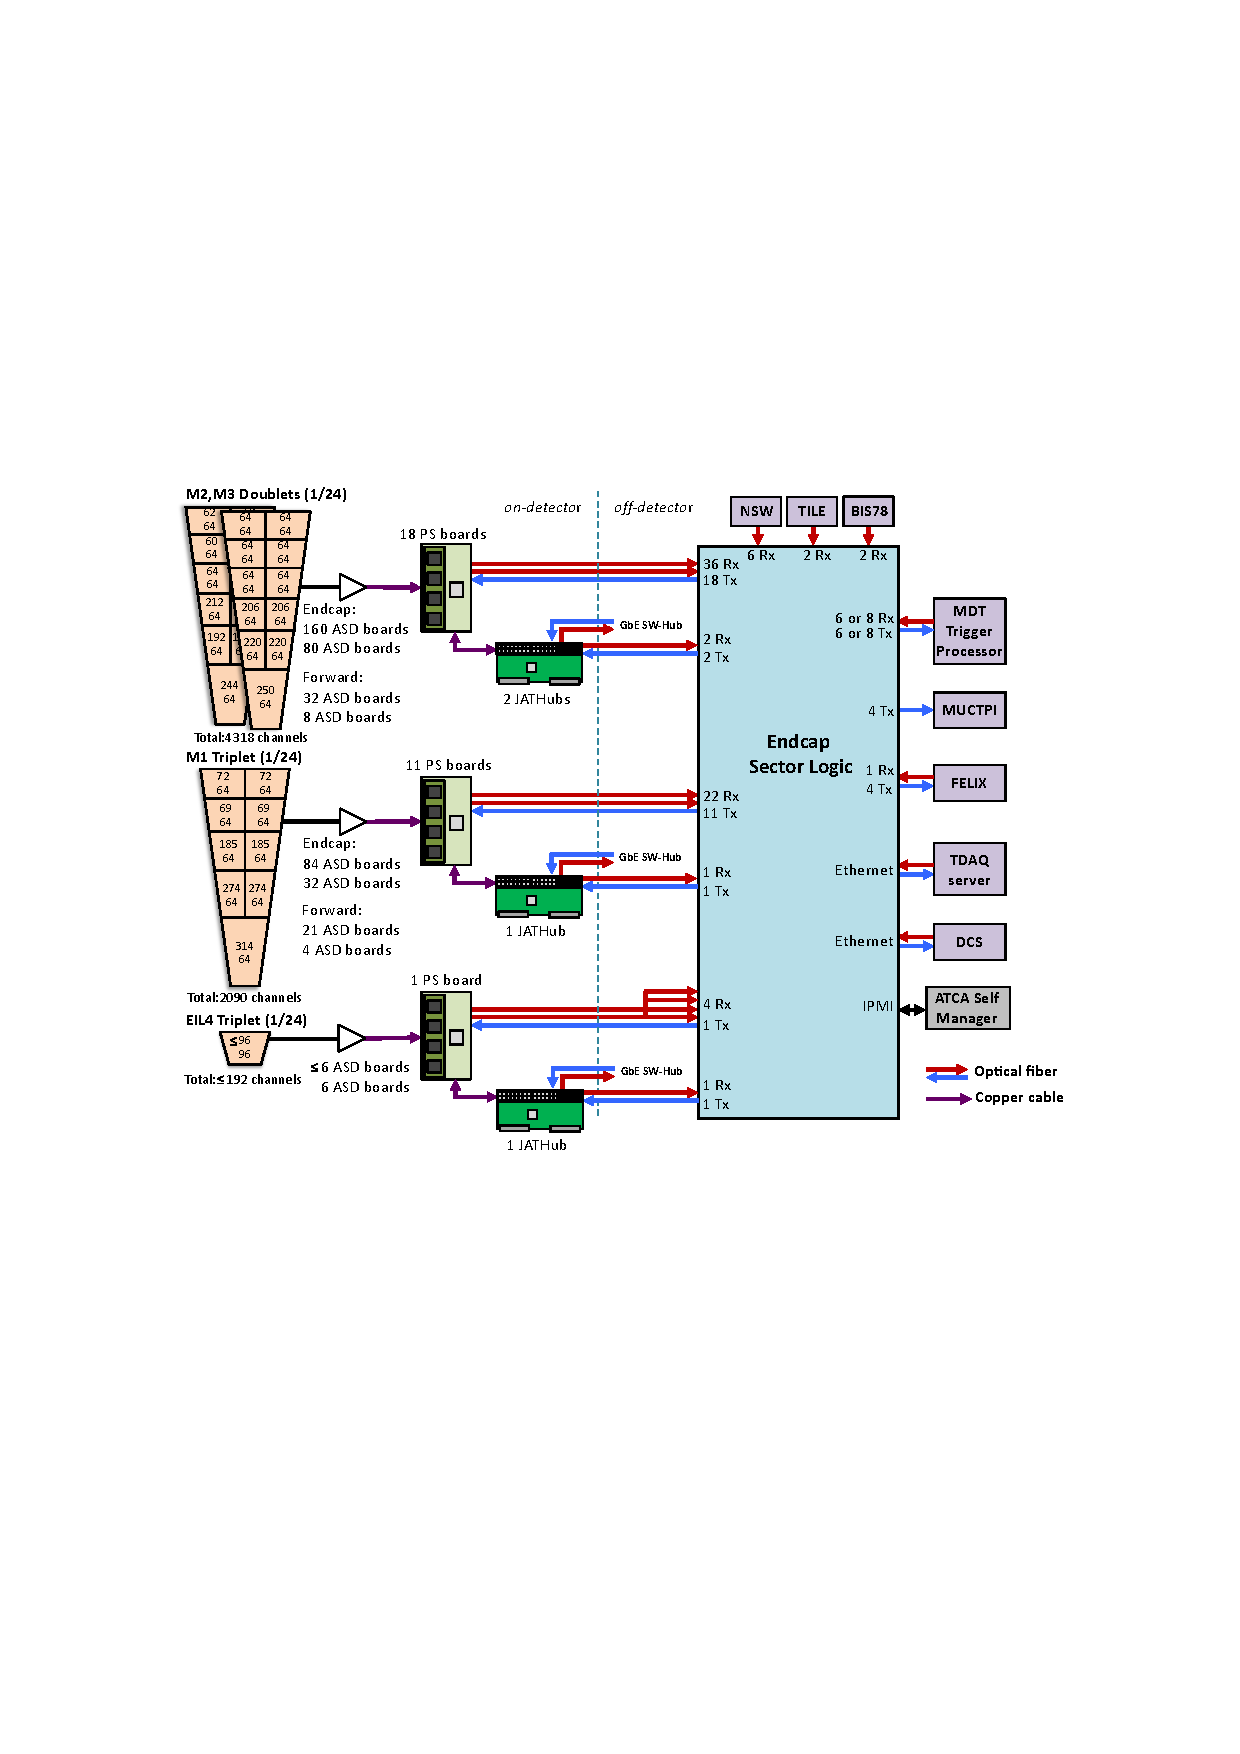
\includegraphics[width=16cm]{fig/Intro/TGC_phase2tdaq.pdf}
\caption[高輝度LHC-ATLAS実験におけるTGC検出器システムの概要]{高輝度LHC-ATLAS実験におけるTGC検出器システムの概要\cite{tdr_phase2muon_2017017}。TGCからの電流信号はASDでデジタル信号に変換され、PS board上のPP ASI で BCIDされる。PP ASICからのヒット信号はヒットの有無に関わらず、PS board FPGA から光ファイバーを通じてSLへ送られる。1枚のSLは1つの1/24セクターを担当し、PS board からのヒット信号に加えてTGC EI、NSW、RPC BIS78、Tile カロリーメーターの情報も利用して$p_{\mathrm{T}}$を判定する。その後SLは再構成した飛跡情報をMDT Trigger Processorに送信し、より精度の高い$p_{\mathrm{T}}$を計算する。SLからのトリガー出力は、MUCTPIを介してCTPへ送信され、L0 トリガー判定が行われる。CTPでL0 トリガー判定を待っている間、衝突データはSLでバッファーされ、L0Aが出されたものはFELIXを通して後段へ読み出される。TTC信号はCTPからFELIXを介して各SLに分配され、PS board へのコントロール信号に乗せられPS boardに分配される。JATHubはデータパスとは独立したモジュールで、PS board の制御を担当する。}
\label{TGC_phase2tdaq}
\end{figure}

トリガー回路および読み出し回路は主にSL上のFPGAに集約される。TGCで生じる電流信号はASDでデジタル信号に変換された後、PS board上のPP ASICでBCIDされる。PP ASICからのヒット信号は、PS board上のFPGAでまとめられ、光ファイバーを通じてSLに送信される。SLは、PS boardから送られるTGC BW 7層の情報に加え、TGC EI、NSW、RPC BIS78、Tile カロリメーターの情報も用いてミューオンの\pt を概算する。その後SLはMDT Trigger Processor (MDTTP) にミューオン飛跡候補を送信し、よりよい分解能で\pt を再構成する。SLのトリガー出力はMUCTPI通じてCTPへ送信され、L0 トリガー判定が行われる。CTPでのトリガー判定を待っている間、ヒットデータはSL内でバッファーされ、L0Aが発行されたバンチ交差事象のデータはFELIXを通じて後段へ読み出される。

TTC信号はCTPからFELIXを通じて各SLに分配され、PS board へのコントロール信号に乗せて各PS board に分配される。JATHubはデータパスと独立しており、PS board の制御を担当する。
このシステムではバックエンドのSLとフロントエンドのPS boardが光リンクのみで接続されており、トリガー、データ読み出し、コントロール、TTCの分配をコンパクトに実現している。

以下にTGC検出器における読み出し、トリガー、制御に関わるそれぞれのエレクトロニクスとその役割を説明する。

        \subsection*{Amplifier-Shaper-Discriminator (ASD)}
    ワイヤー、ストリップからの電流信号はTGCのチェンバーに直接取り付けられた、Amplifier-Shaper-Discriminator  (ASD) ボードで電圧信号に変換された後に増幅され、閾値電圧との比較による信号識別を経て、最終的にLVDS規格のデジタル信号へ変換される。図\ref{TGC_ASD}にASDの概要を示す。ASDはチャージアンプである前段増幅器 (Preamplifier)、差動電圧増幅回路、コンパレーターから構成されている。前段増幅回路では、0.8 V/pCのゲインを用いて、16 nsの時定数で電流信号を電圧信号に変換する。その信号は差動電圧増幅回路で7倍に増幅され、コンパレーターで閾値電圧を超えている時間に対応するパルス長のLVDS信号に変換される。この閾値電圧はPS boardから設定できるようになっている。またASDにはTGCのチャージ出力をエミュレートするTest Pulse源が実装されており、ASD以降のトリガー・データパスの試験に利用される。1枚のASDボードには4枚のASDチップが搭載されており、1枚あたり4チャンネル、全部で16チャンネルの信号を処理する。TGCの読み出しチャンネルはおよそ32万チャンネルであるため、システム全体ではおよそ2万枚のASDボードが設置される。

    \begin{figure}
    \begin{minipage}[b]{.5\linewidth}
    \centering
    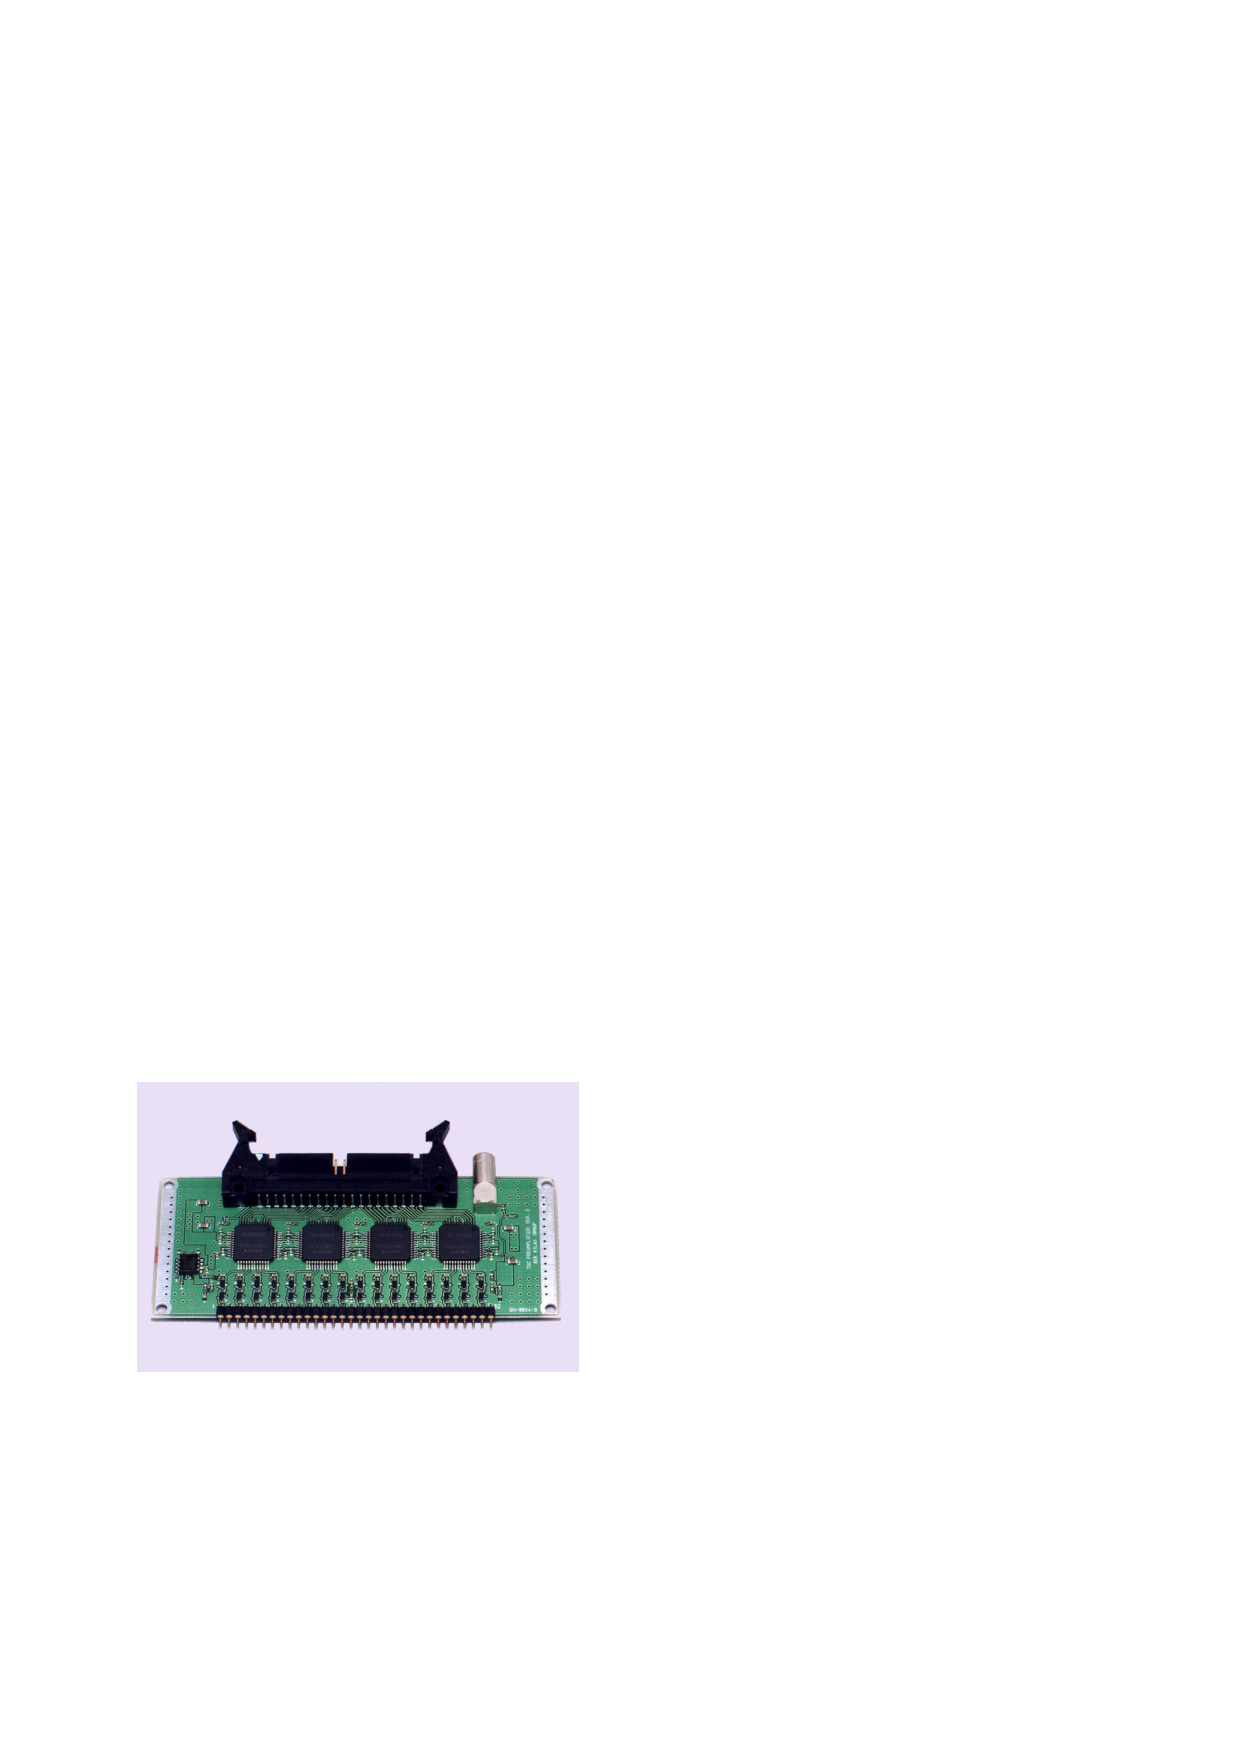
\includegraphics[height=5cm]{fig/Intro/TGC_ASD.pdf}
    \subcaption{ASDボードの写真}
    \end{minipage}%
    \begin{minipage}[b]{.5\linewidth}
    \centering
    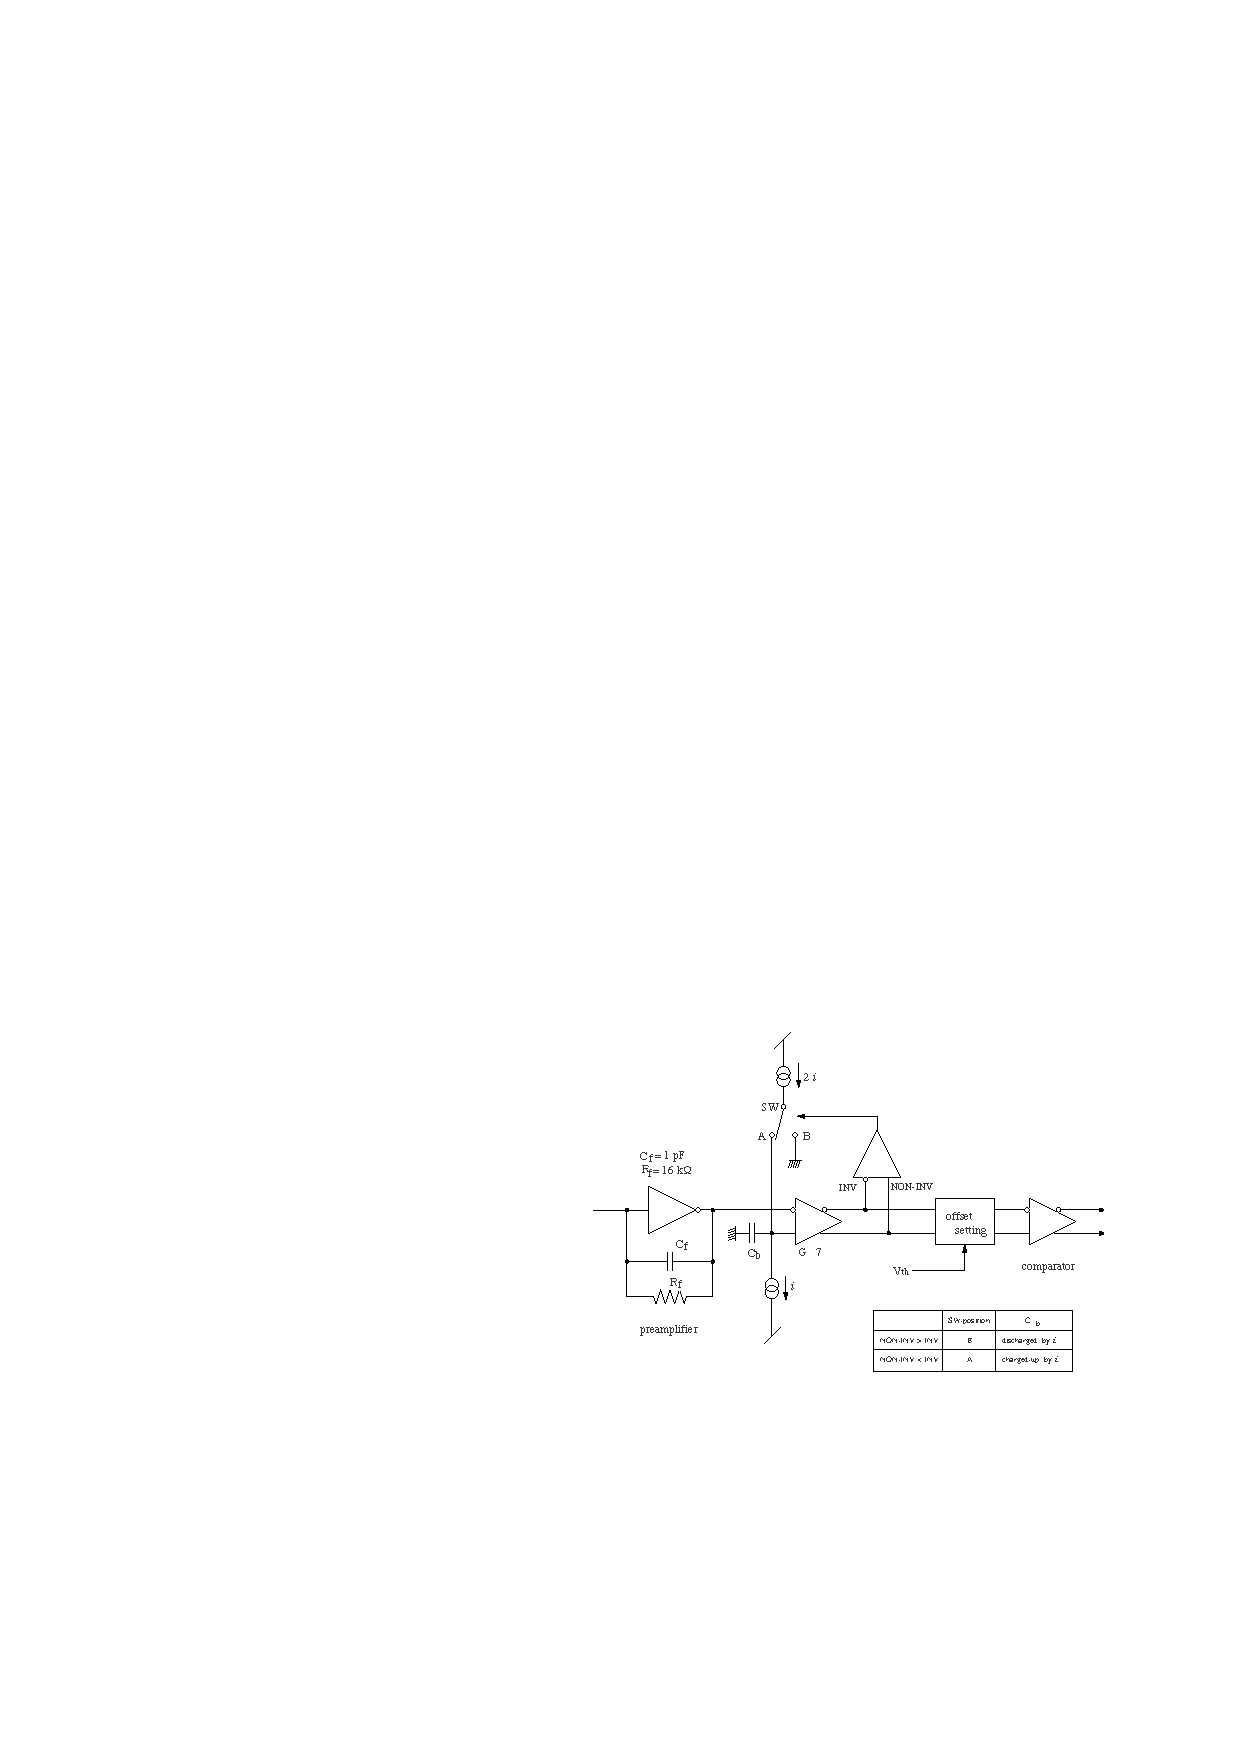
\includegraphics[height=5cm]{fig/Intro/TGC_ASDcircuite.pdf}
    \subcaption{ASDチップの回路ブロック図}
    \end{minipage}%
    \caption[ASDの概要]{ASDの概要\cite{ASD}。(a)にASDボードの写真を示す。1枚のASDボードには4枚のASDチップが搭載されており、1つにつき4チャンネル分のヒット信号を処理する。(b)にASDチップの回路図を示す。ASDチップは前段増幅回路、差動電圧増幅回路、コンパレーターから構成される。}
    \label{TGC_ASD}
    \end{figure}

        \subsection*{Primary ProceSsor board (PS board)}
    ASDボードからのヒット信号は、次にPS boardに送られる。PS boardはPP ASICとXilinx 社製のKintex-7 FPGAという2 種類の集積回路を搭載している。PP ASICは可変遅延機能により各ASDからの入力信号の到着時間を揃え、その信号がどの陽子バンチ交差に由来するかを識別する (BCID)。PS board FPGAはBCIDされたヒット信号を高速光シリアル通信に乗せてSLへ転送する。図\ref{TGC_PSB}にPS boardの最終試作機の写真とブロック図を示す。PS boardには8つのPP ASIが搭載され、そのうち4つはメザニンカードに乗せられる。1つのPP ASICは2台のASDと接続され、合計で32チャンネルの信号を処理する。PS board FPGAは8つのPP ASICからのヒット信号をまとめて、合計256チャンネル分のヒットビットマップをSLに送る。

    PS boardはボード上にDAC  (Degital Analog Converter) 、ADC  (Analog Degital Converter) 、クロックジッタークリーナー、QSPIフラッシュメモリーなどの電子素子を搭載している。DACはASDのコンパレーターにアナログの閾値電圧を供給する。PS board FPGAから閾値電圧の大きさを設定することができる。ADCはDACから供給される閾値電圧をモニターする。クロックジッタークリーナーは、PS board FPGAがシリアルデータから再構成したLHCバンチ交差クロックのジッターを低減する。QSPI フラッシュメモリーは不揮発性のメモリーで、ボードの電源が落とされた場合でも書き込まれた値を保持することができる。これを利用して、PS board FPGAのファームウェアや、ボードごとに最適化されたPP ASICの遅延値などのパラメーターを保存する役割を果たす。また、インターフェイスとして、電気信号を光信号に変換するSFP+モジュール、Cat-6ケーブルのコネクターであるRJ45を有しており、それぞれSLとJATHubに接続される。
    
    PS board はTGCシステム全体で1434 枚設置され、それぞれの個体の量産が2024 年から始まる。本研究では、量産される各個体にハードウェアの不具合がないことを検証する品質保証試験の設計、およびそれに向けた機能開発を行なった。これに関する詳細は\ref{chap_QAQC}章で議論する。
    以下にPP ASICとPS board FPGAの役割について詳しく説明する。

    \begin{figure}
    \begin{minipage}[b]{.5\linewidth}
    \centering
    \includegraphics[height=8cm]{fig/Intro/TGC_PSB.pdf}
    \subcaption{PS boardの写真}
    \end{minipage}%
    \begin{minipage}[b]{.5\linewidth}
    \centering
    \includegraphics[height=8cm]{fig/Intro/TGC_PSBblock.pdf}
    \subcaption{PS boardのブロック図}
    \end{minipage}%
    \caption[PS boardの概要]{PS boardの概要。1枚のPS board は、1つのFPGAと8つの PP ASIC (メインボードに4個、メザニンボードに4個)を搭載している。1つのPP ASICは2台のASDと接続され、合計で32チャンネルの信号を処理する。また、PS board はDAC、ADC、クロックジッタークリーナー、QSPIフラッシュメモリーなどの素子を搭載しており、これらはPS board FPGAからコンフィギュレーションすることができる。}
    \label{TGC_PSB}
    \end{figure}

    \subsubsection*{Patch-Panel ASIC (PP ASIC)}


    \begin{figure} 
    \centering
    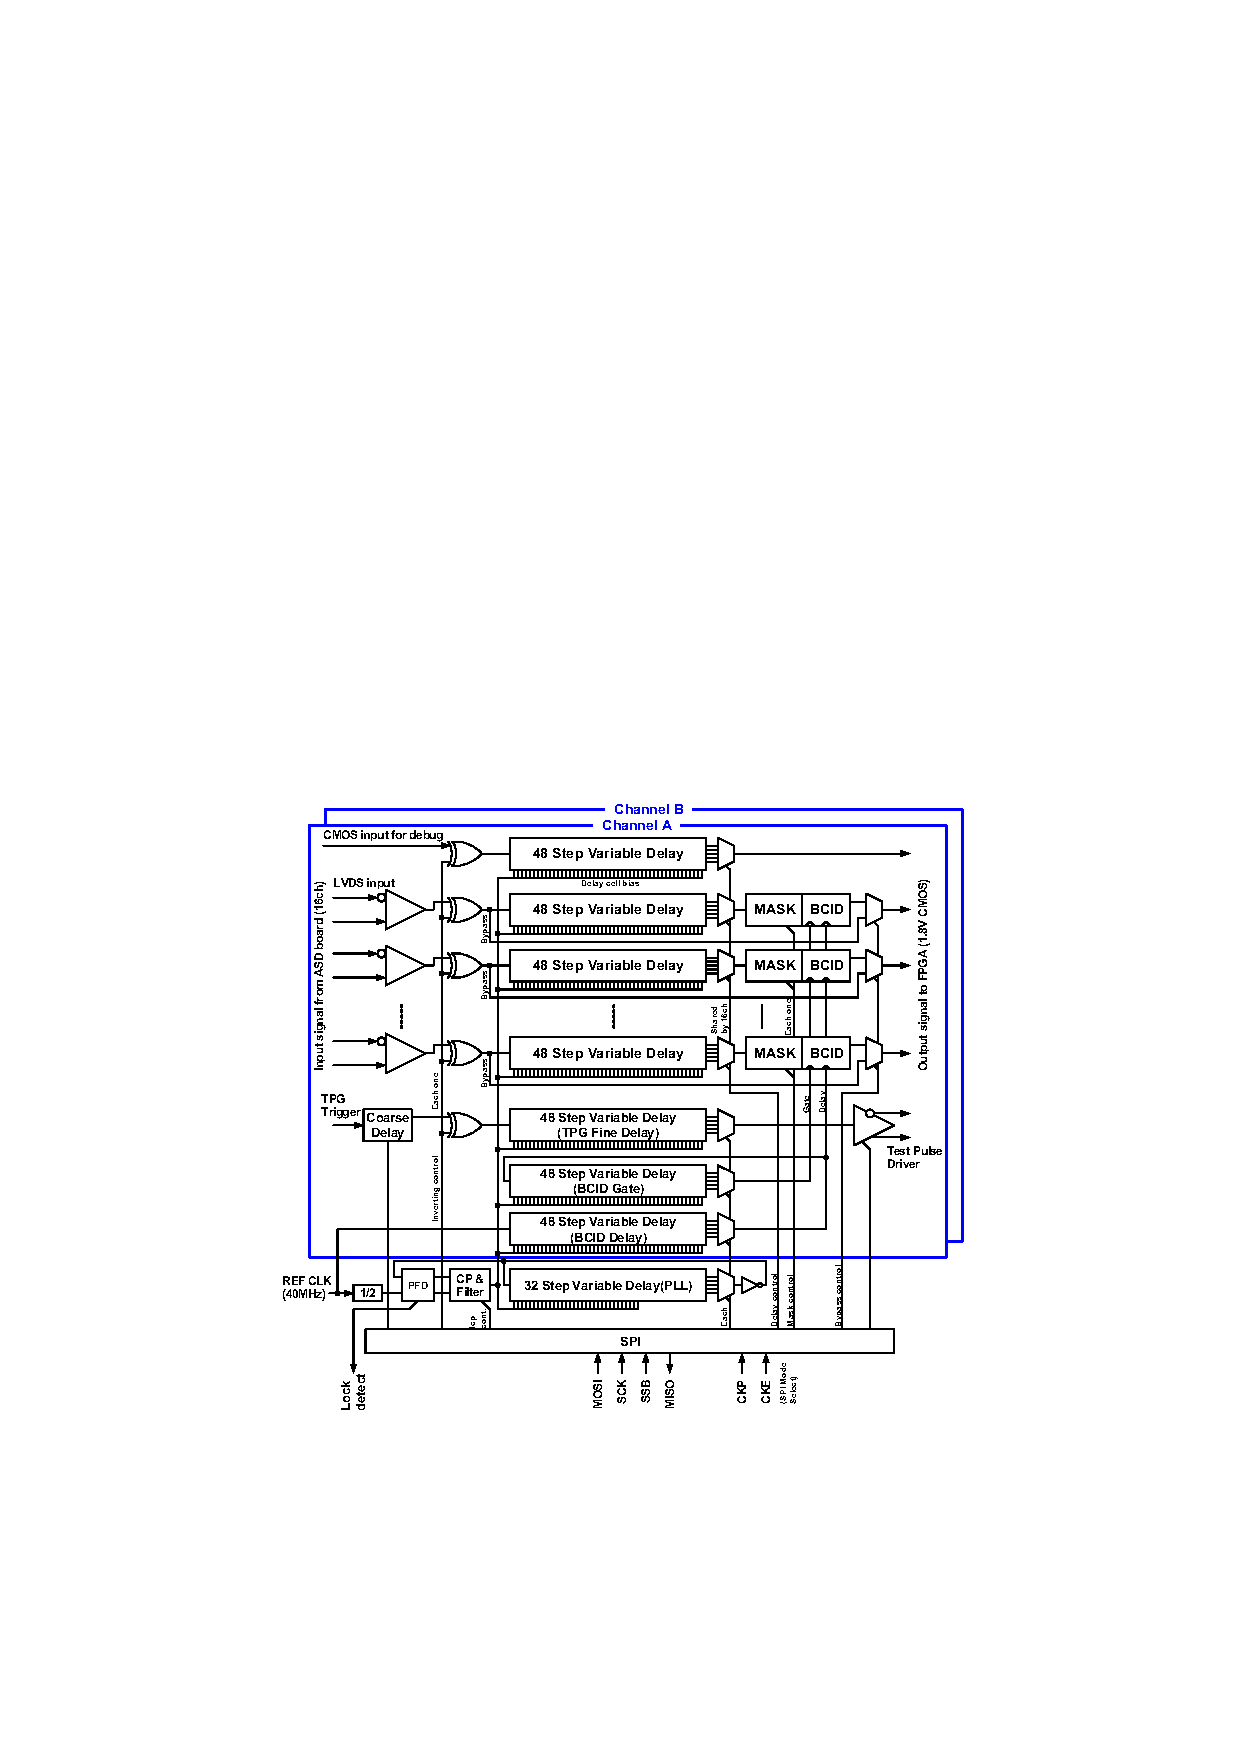
\includegraphics[width=16cm]{fig/Intro/TGC_PPASIC.pdf}
    \caption[PP ASIC回路のブロック図]{PP ASIC回路のブロック図\cite{PPASIC}。Channel AとChannel Bがそれぞれ1つのASDボードに対応し、1つの PP ASICは32チャンネルのLVDS信号を受け取る。PP ASICは主に可変遅延回路と陽子バンチ識別回路で構成され、この2つを用いてBCIDを行う。}
    \label{TGC_PPASIC}
    \end{figure}

    図\ref{TGC_PPASIC}にPP ASICのブロック図を示す。PP ASICは主に可変遅延回路と陽子バンチ識別回路で構成される。PP ASICがASDから受け取るLVDS信号の入力時間には、チャンネルごとに$\mathcal{O}(10\,\mathrm{ns})$のばらつきが存在する。これは、衝突点から検出器までの飛行時間 (Time-of-Flight) や、ASDからPP ASICまでのLVDSケーブルの長さがチャンネルごとに異なるためである。また、同一チャンネル内でもイベントごとに信号の到着時間が20 $\sim$ 30 ns 程度変動する (図\ref{TGC_fructuation})。これは、ミューオンの入射位置に応じて、電荷が検出される位置からASDまでの距離が異なり、結果として信号の伝播遅延や電荷のドリフト時間にばらつきが生じるためである。

    \begin{figure} 
    \centering
    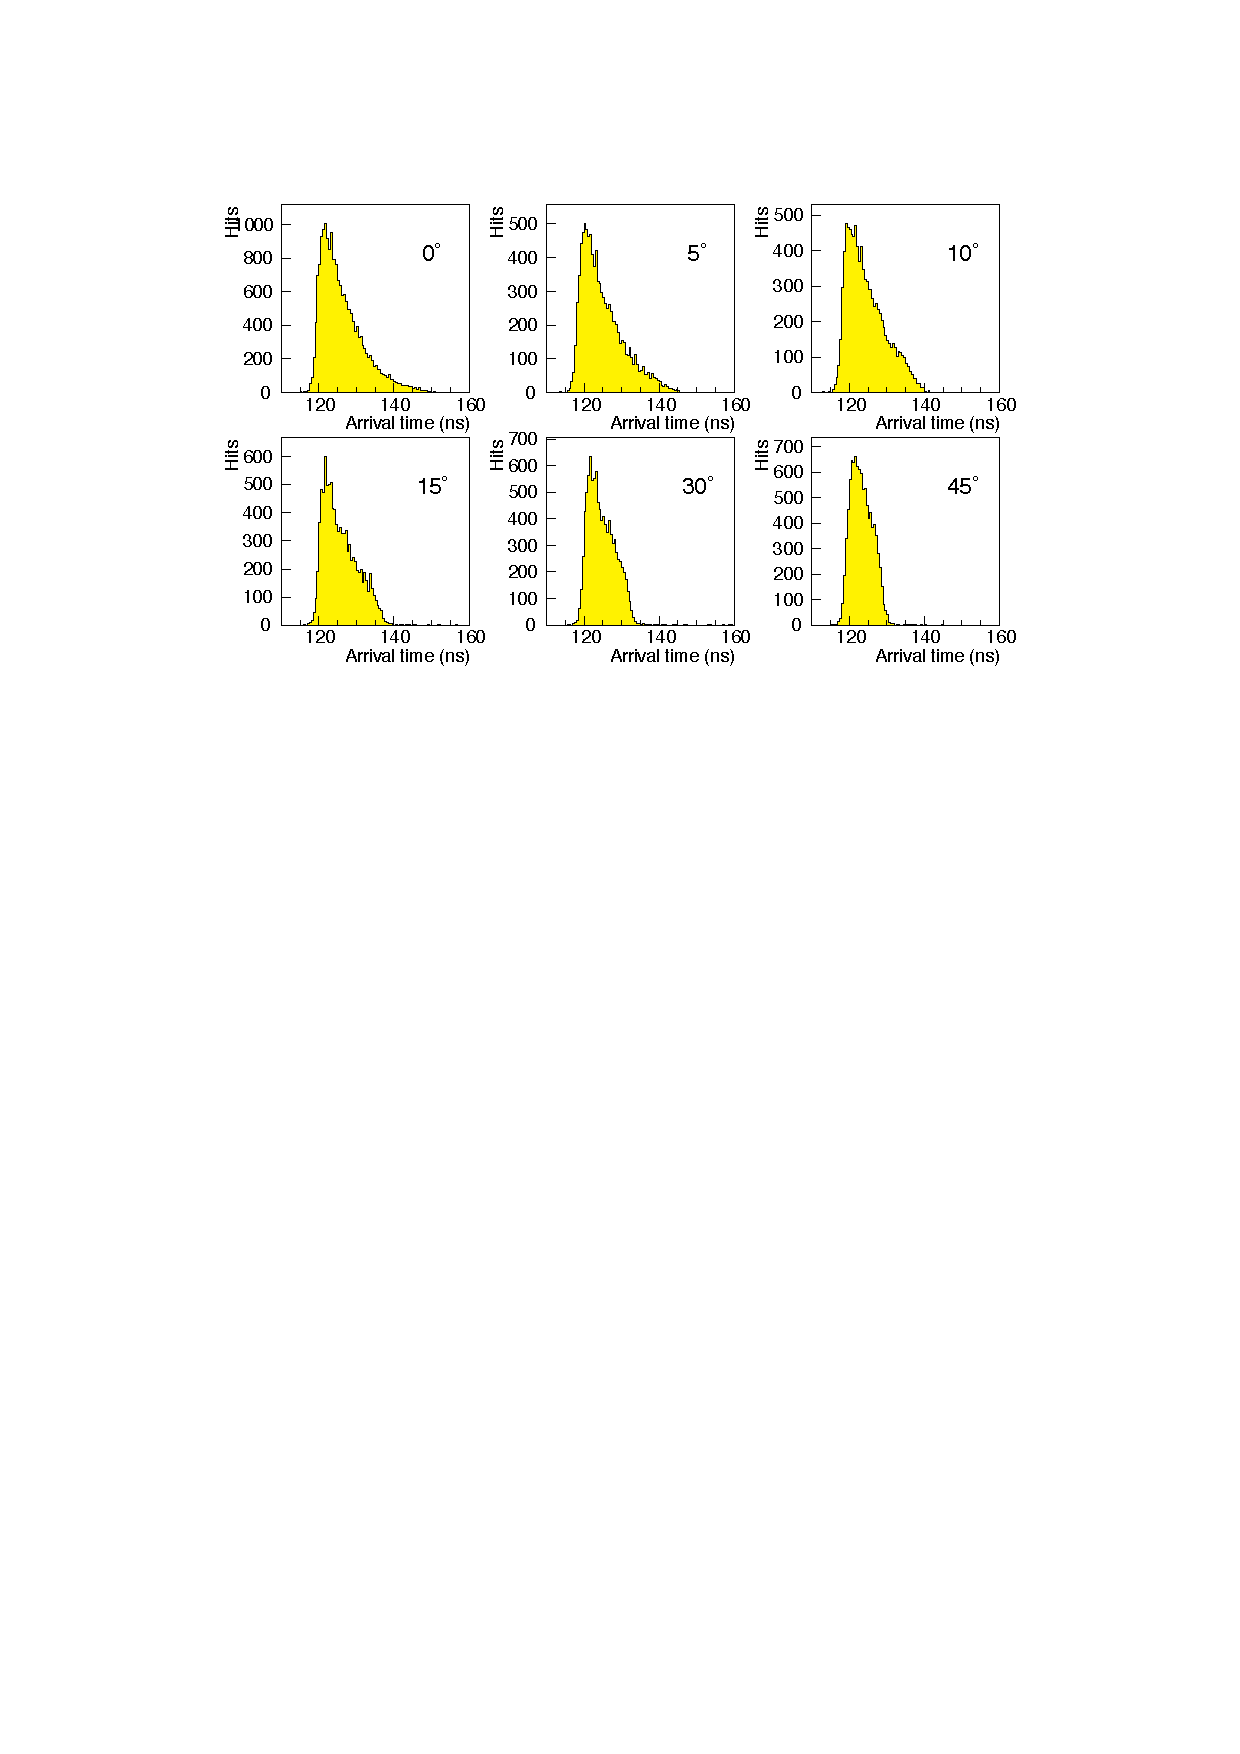
\includegraphics[width=16cm]{fig/Intro/TGC_fructuation.pdf}
    \caption[ミューオンがTGC検出器に入射してから、ASDに信号が到着するまでの時間分布]{ミューオンがTGC検出器に入射してから、ASDに信号が到着するまでの時間分布\cite{TGC_fructuation}。時間分布はミューオンが入射する角度に依存して、20 $\sim$ 30 nsの幅を持つ。}
    \label{TGC_fructuation}
    \end{figure}

    このばらつきを揃えるために、各ASDごとに固有の遅延を加えるのが可変遅延回路である。可変遅延回路は1 ns以下の刻み幅で、最大45 nsまでの遅延をかけることができる。PP ASICに一番遅く到着するASDからの信号の立ち上がりに、他のASDからの信号の立ち上がりを合わせるように遅延パラメーターが設定される。この遅延パラメーターはPS boardのFGPAから設定可能である。

    可変遅延回路でタイミングが揃えられた後、信号は陽子バンチ識別回路に送られる。陽子バンチ識別回路は、PP ASICに入射するデジタル信号の立ち上がりを検出し、その信号がどの陽子バンチ交差に由来するのか識別する。陽子バンチ回路の概念図を図\ref{TGC_BCID}に示す。前述の通り、同じチャンネル内であってもヒット信号の到着時間はイベント毎に20 $\sim$ 30 ns程度の幅を持ち、この時間幅のうちに来るヒット信号には同じBCIDを付与する必要がある。そのため、同じBCIDを付与する時間幅 (有効ゲート幅) をASDごとに設定できるようになっており、信号到着時間幅が25 nsを超える場合に対応するため、有効ゲート幅は25 ns以上に設定できるようになっている。その場合、2つの有効ゲートが重なる時間が存在するが、このタイミングに入射した信号には2バンチ分の信号が出力される。有効ゲート幅もPS boardのFPGAから設定することができる。

    \begin{figure} 
    \centering
    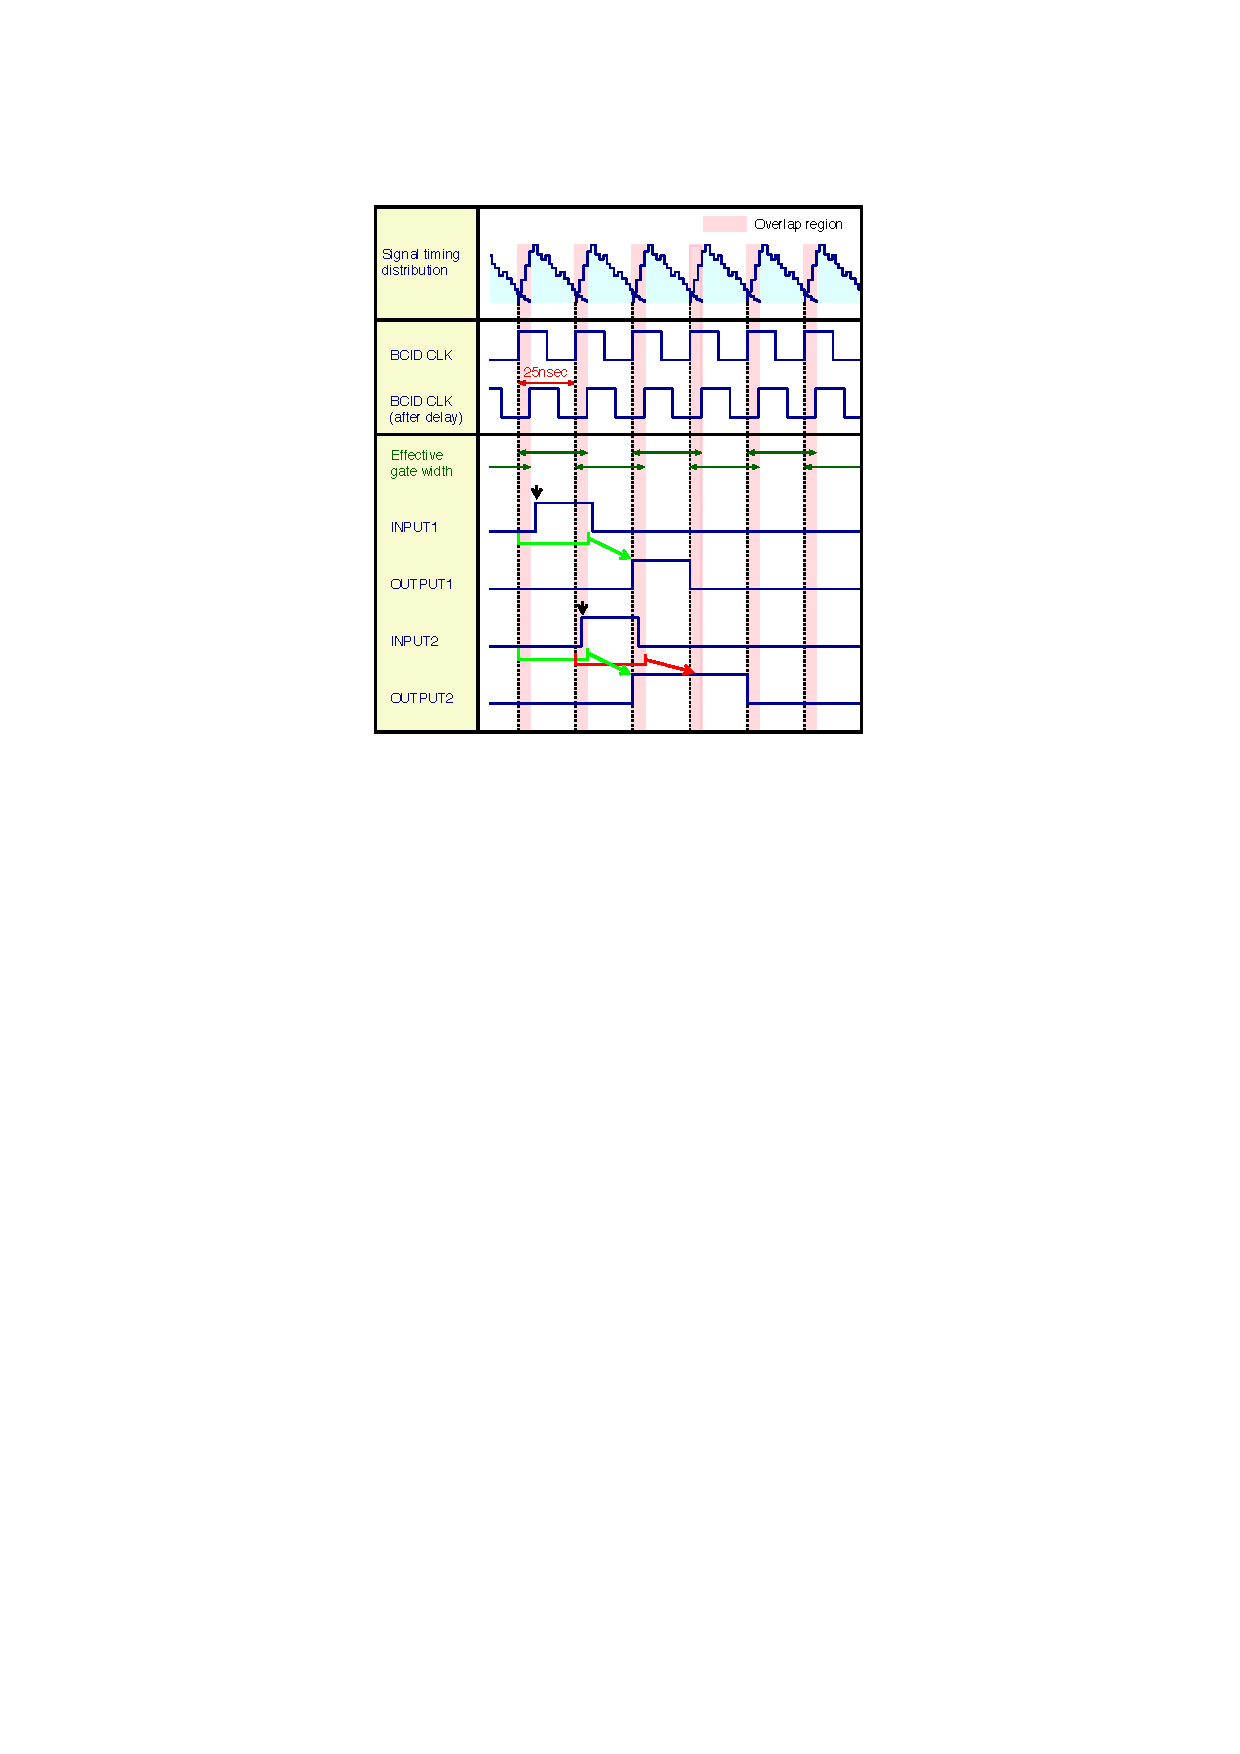
\includegraphics[width=14cm]{fig/Intro/TGC_BCID.pdf}
    \caption[陽子バンチ識別回路のタイミングチャート]{陽子バンチ識別回路のタイミングチャート\cite{mt_takemoto}。BCID CLKの立ち上がりのタイミングでINPUTがhighであった時、次のBCID CLKから1 BC分デジタル信号が出力される(図のINPUT1の場合に対応)。BCID CLKの立ち上がりのタイミングが有効ゲートが重なる領域に来た場合には、2 BC分のデジタル信号を出力する(図のINPUT2の場合に対応)。}
    \label{TGC_BCID}
    \end{figure}

    \subsubsection*{PS board FPGA}

    PS board FPGAはSLにヒットデータを送信することに加えて、PS board上の各素子の制御/監視およびLHCバンチ交差クロックの再構成を担当する。
    PP ASICによりLHCバンチ交差クロックと同期された256チャンネルのヒット信号は、PS board FPGAでまとめられ、光ファイバーを通じてSLに転送される。
    PS boardからSLに送信されるデータフォーマットを図\ref{TGC_PSBuplink}に示す。256チャンネルのヒットデータに加え、64 bitのヘッダーが付与され、合計320 bitのデータが25 nsおきに送信される。320 bitのデータは2本の光ファイバーに分けられ、32 bitごとにワードという単位でまとめられる。ワード0ではヘッダーが、ワード1 $\sim$ 4にはヒットデータが詰められる。データ転送は高速シリアル通信で行われ、FPGA内のパラレルデータをシリアルデータに変換する際には8b10bコーディングが用いられる。そのため、1本の光ファイバーのラインレートは$160 \, \mathrm{bit} \times 10/8 \times 40 \mathrm{\,MHz} = 8 \,\mathrm{Gbps}$となる。

    \begin{figure} 
    \centering
    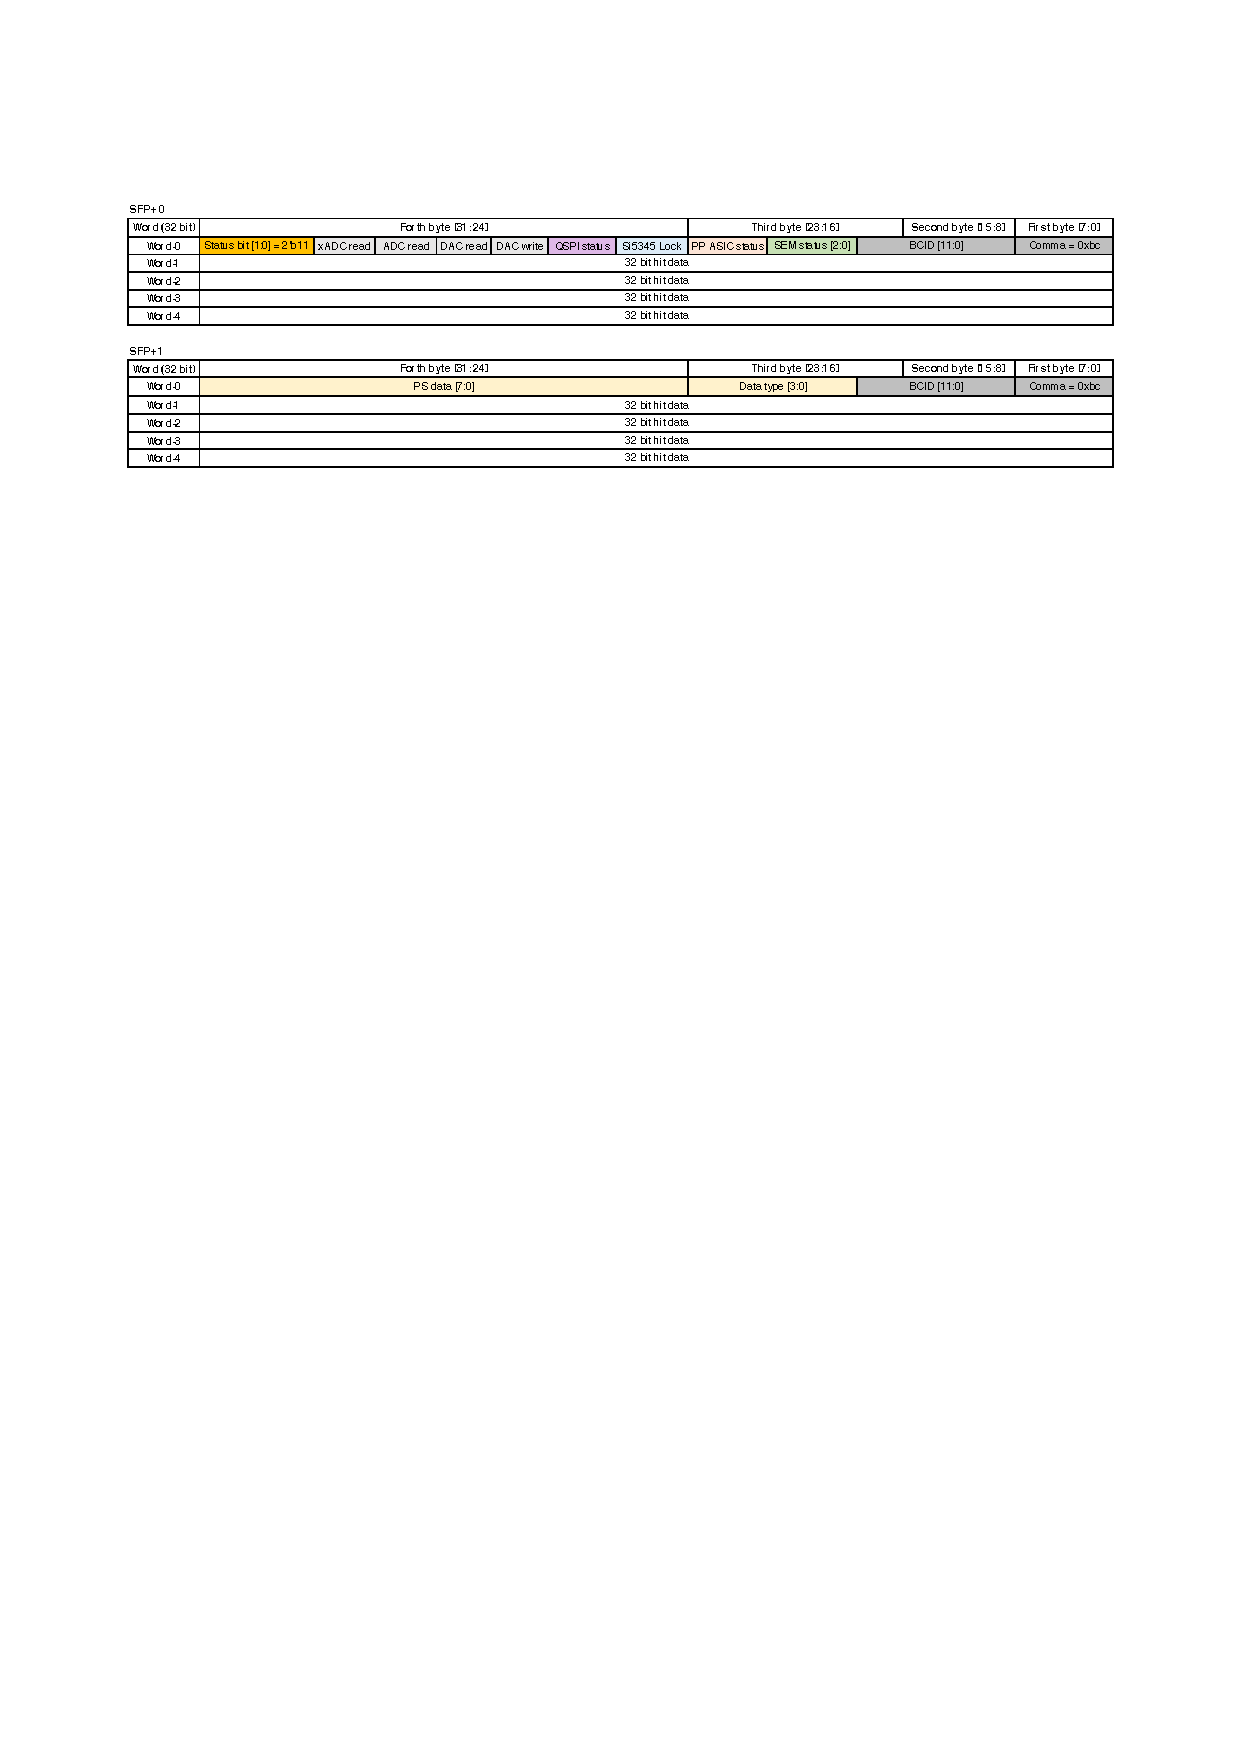
\includegraphics[width=16cm]{fig/Intro/TGC_PSBuplink.pdf}
    \caption[PS boardからSLへ送るデータフォーマット]{PS boardからSLへ送るデータフォーマット\cite{mt_aoki}。256チャンネルのヒットデータに64 bitのヘッダーが付与された、合計320 bit のデータが2リンクに分けられ、25 nsおきに送信される。ヘッダーワードには主にPS board FPGAやその他の素子の状態を表すモニター用のデータが含まれる。}
    \label{TGC_PSBuplink}
    \end{figure}

    PS board FGPAはSLからのコントロール信号を1本の光ファイバーを通じて受け取る。コントロール信号のデータフォーマットを図\ref{TGC_PSBdownlink}に示す。SLはワード2と3で定義されたAddress、Data、Commandを利用してPS board FPGA内のレジスタを操作する。PS board FPGAとQSPIフラッシュメモリーはSPIバスで接続されており、SLがFPGAを介してSPIバスを制御することで、QSPIフラッシュメモリーにデータを書き込むことができる。この通信パスを利用して、PP ASICの遅延パラメーターや有効ゲート幅、ASDに供給する閾値電圧などの制御用パラメーターをQSPI フラッシュメモリー上に保存することができる。

    PS board FPGAはQSPIフラッシュメモリーに保存された制御用パラメーターを読み取り、PP ASIC、ASDに自動で分配する。これを自立型制御機構と呼ぶ。この機構により、1434 枚のPS boardには同じファームウェア\footnote{正確にはPS boardからSLに送るデータフォーマットに3種類のバラエティが必要であるため、3種類のファームウェアを使い分けることになる。}を使用し、ボード毎に異なるパラメーターの設定は各個体が自動で行う、という次世代的な制御モデルを実現している。
    PS board FPGA にはPS board上の素子の状態を監視するための機構も備わっており、DACに分配した設定値、ADC、xADC\footnote{Xilinx Analog-Digital Converter、FPGA内部の温度、電源電圧、外部からのアナログ信号を監視するためのモジュール。PS boardに供給される3.3 VD  (デジタル) 、+ 3 VA  (アナログ) 、-3 VAをモニターする}のモニター値、GTXトランシーバーのロック信号を定期的に読み出し、SLに送信する。これによりSLはフロントエンドのPS boardの状態を常に把握し、異常が生じた際には瞬時に対応することができる。

    \begin{figure} 
        \centering
        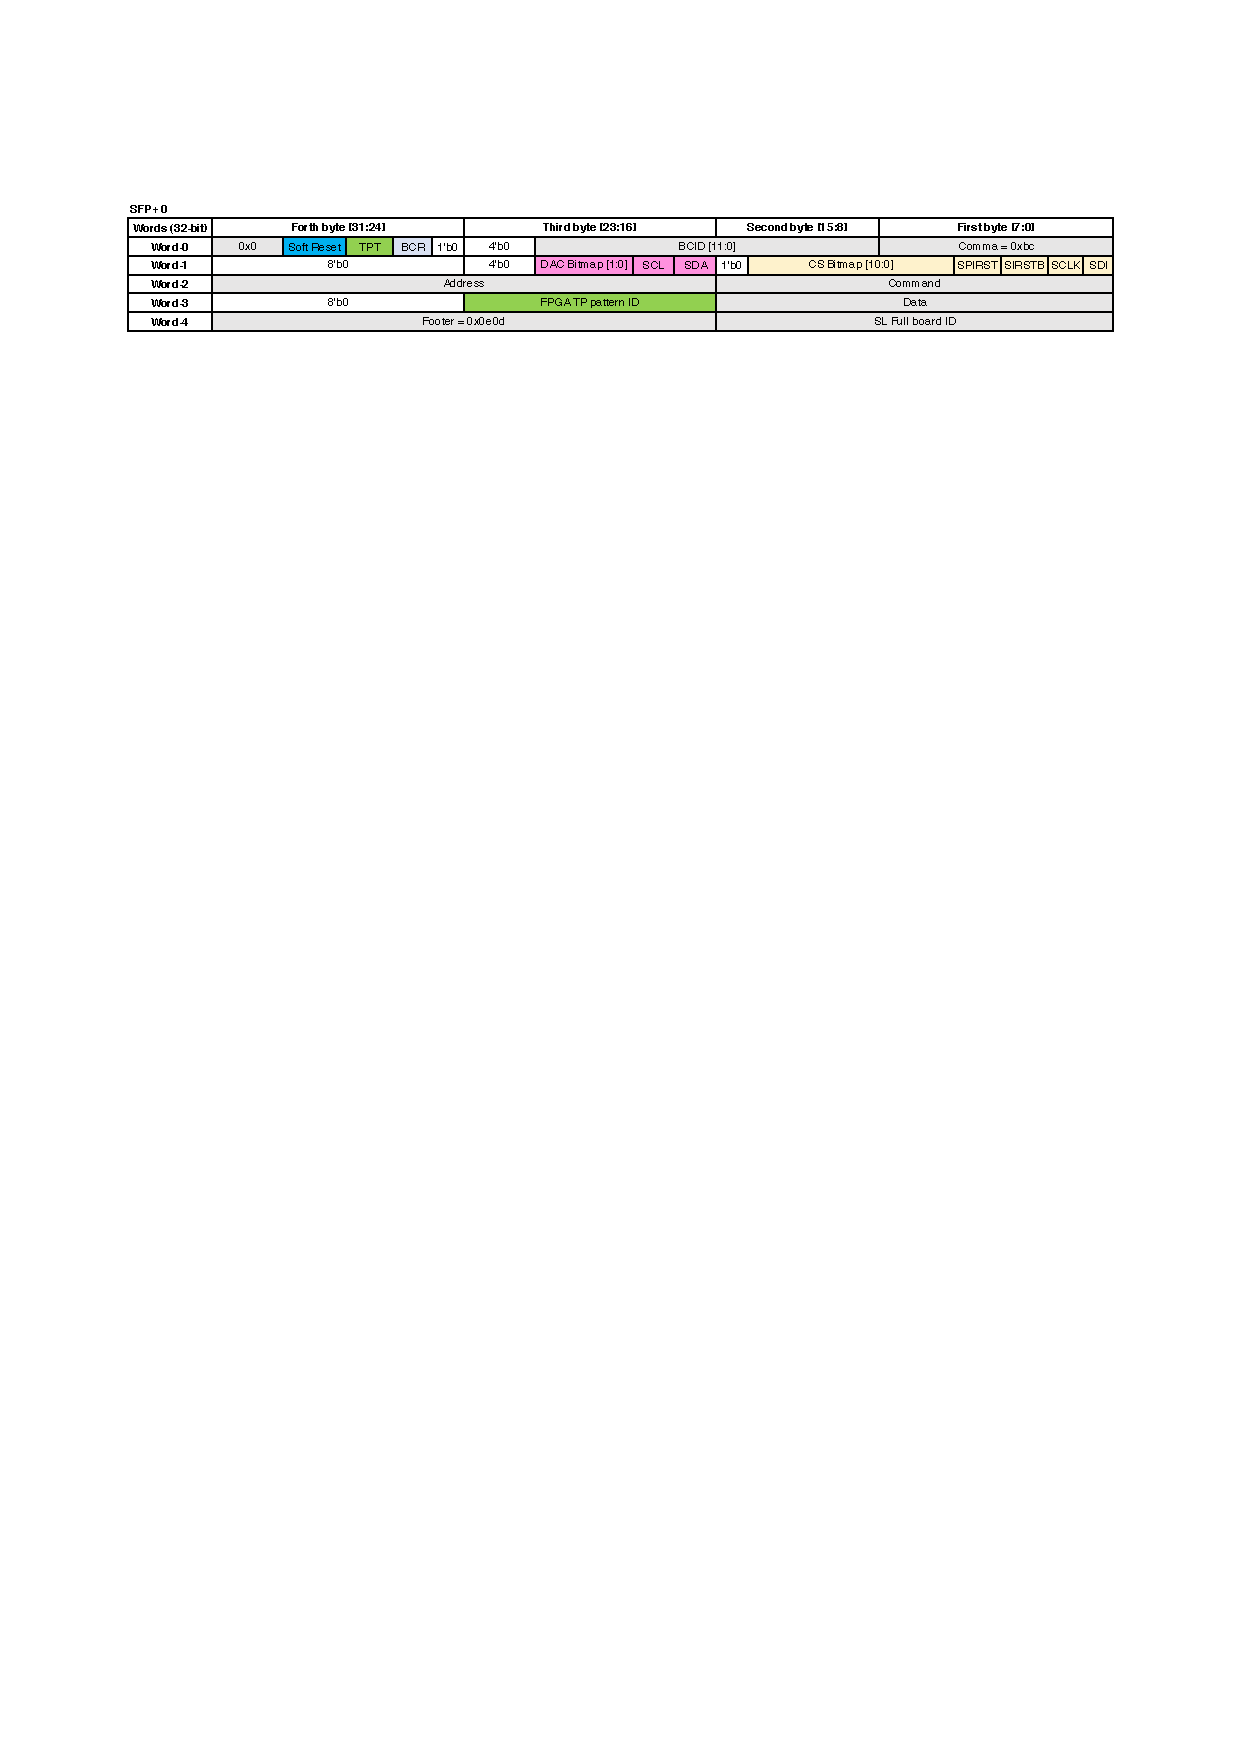
\includegraphics[width=16cm]{fig/Intro/TGC_PSBdownlink.pdf}
        \caption[SLからPS boardへ送るコントロールデータのフォーマット]{SLからPS boardへ送るコントロール信号のデータフォーマット\cite{mt_aoki}。Word 0にはTTC信号、Word 1にはビットバンギング用のデータ、Word 2、Word 3にはPS board FPGA内のレジスタ操作用のデータが含まれる。}
        \label{TGC_PSBdownlink}
    \end{figure}
    
    TTC信号もこのコントロール信号に乗せられてPS boardに分配される。PS boardのGTXトランシーバーは、ワード0で定義されるComma ワードを使用して、シリアルデータからLHCバンチ交差クロックを再構成する。PS boardで再構成されたLHCバンチ交差クロックはPS board 間で位相を揃えるための適切な遅延が加えられた後、ジッタークリーナーを経由してFPGA、GTXトランシーバー、PP ASICへ分配される。    

    さらに、PS boardは放射線損傷に対する堅牢性を実現するシステムを搭載している。PS boardは実験室に置かれるため、FPGAは電子回路上のメモリのビットが反転してしまうSingle Event Upset (SEU) などの放射線損傷を受ける可能性がある。先行研究\cite{PSB_SEU}によると、1つのPS board FPGAでは3時間に一回程度SEUが発生する。FPGAには修復可能なSEU  (1ビットエラーおよび隣接する2ビットエラー)を自動的に修復するSoft Error Mitigation Controller  (SEM) が実装されている。また修復不可能なSEU  (隣接しない2ビットエラーおよび3ビット以上のエラー) が生じた際には、PS boardの制御を担当するJATHubに対して救難信号を送り、JATHubにFPGAの再コンフィギュレーション用の信号を送信させることでこれに対処する。このように、放射線損傷に対して堅牢なシステムを実現することで、データ取得時のデッドタイムを最小限に抑えることができる。    

        \subsection*{JTAG AssisTance Hub (JATHub)}
    JATHubはデータパスとは独立した、PS board制御用の回路である。概要を図\ref{TGC_JATHub}に示す。JATHubはXilinx社製のZynq-7000 SoCをメインドライバーとして搭載する。Zynqはプロセッサー部分であるProcessing System  (PS) と、FPGA部分であるProgrammable Logic  (PL) で構成されている。PS部分ではLinuxなどのカーネルを立ち上げることが可能で、C言語などで記述されたアプリケーションを実行してFPGAを操作することができる。

    JATHubはインターフェイスとして、PS boardとLVDS通信するためのRJ45コネクターと、イーサーネット通信を行うためのSFP+モジュールを搭載している。1枚のJATHubは最大で11枚のPS boardと接続可能であり、それぞれ2本のCat-6\footnote{Category-6 twisted pair cable。4対8線の動線で構成されており、4種類の差動信号線を束ねている。}ケーブルで接続される。一本のCat-6ケーブルはJTAG線と呼ばれ、JATHubを起点に遠隔でPS boardのファームウェアを書き込む際に利用される。
    もう1本のCat-6ケーブルはRecovery/Monitor線と呼ばれ、PS boardの放射線損傷に対する回復、およびLHCバンチ交差クロックのモニターに利用される。
    
    図\ref{JATHubsem}にJATHubのRecovery/Monitor線の概要を示す。PS board FPGAで自己修復不可能なSEUが生じた場合、Recovery Request線 (RcvB線) を通じて救難信号が出される。JATHubは救難信号を受け取ると、PS boardにFPGA再コンフィギュレーション用のProgram信号 (PROGB線) を送信する。この一連の手続きをリカバリー手続きと呼ぶ。Monitor線 (MON) はPS boardが再構成したLHCバンチ交差クロックをJATHubに送信するために利用される。JATHubは接続されるそれぞれのPS boardで再構成されたクロックの位相をモニターし、その位相差を測定する。
    
    PS board の量産試験について議論する\ref{chap_QAQC}章では、JATHubのPS領域とPL領域には実験本番とは異なるシステムを実装し、JATHubをコンパクトなDAQシステムとして利用する。このシステムの詳細は\ref{sec_QAQC_JATHub}節で説明する。



    \begin{figure} 
        \centering
        \includegraphics[width=16cm]{fig/Intro/TGC_JATHub.pdf}
        \caption[JATHubの写真]{JATHubの写真\cite{mt_aoki}。JATHubはメインドライバーとしてCPUとFPGAが統合されたSoCデバイスであるZynq-7000を搭載している。PS board とのインターフェイスとしてLVDS通信用のRJ45コネクターと、イーサーネット通信用のSFP+モジュールを持つ。Mini-Rack内のVMEクレートに設置されるため、VME コネクターを有している。}
        \label{TGC_JATHub}
    \end{figure}

    \begin{figure} 
    \centering
    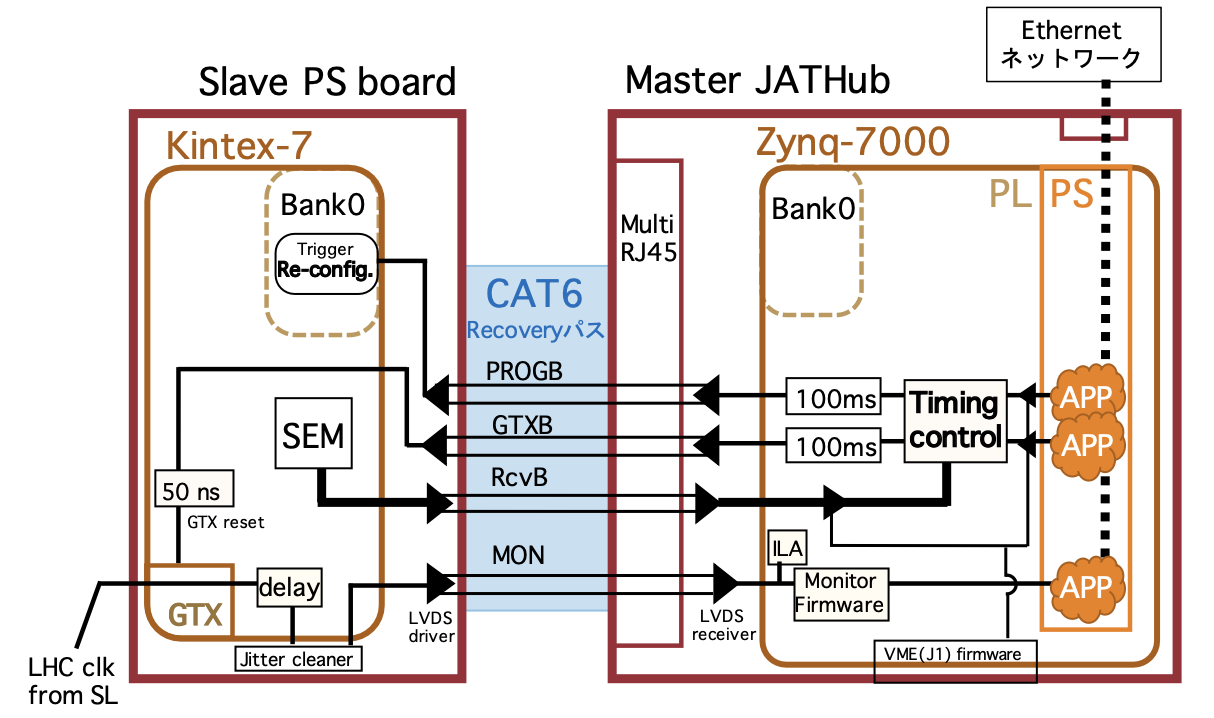
\includegraphics[width=16cm]{fig/QAQC/JATHubsem.png}
    \caption[JATHub によるリカバリー手続きの概要]{JATHub によるリカバリー手続きの概要\cite{mt_atanaka}。PS board に自己修復不可能な SEU 事象が発生した場合、Recovery Request線(RcvB線)を通じてJATHubに救難信号が発出される。これを受信したJATHubはProgram線(PROBG線)を通じてリセット信号を送ることでPS board FPGAの再コンフィギュレーションを行う。}
    \label{JATHubsem}
    \end{figure}

        \subsection*{Sector Logic  (SL) }
PS board から出力されたTGC BW 全7層分のヒットデータはSLに集められる。SLはVirtex UltraScale+ FPGAという大規模FPGAとZynq UltraScale+ MPSoCの2種類の集積回路を搭載している。Virtex UltraScale+ FPGAのデバイスはSL FPGAと呼ばれ、PS boardから受信したヒットデータを用いてトリガー計算を行う。また、SL FPGAはCTPからL0Aが発行されるまでのデータのバッファリングおよ読み出しも担当する。Zynq UltraScale+ MPSoCはVirtex UltraScale+ FPGAやPS boardのコントロールマスターとして機能する。

\begin{figure} 
    \centering
    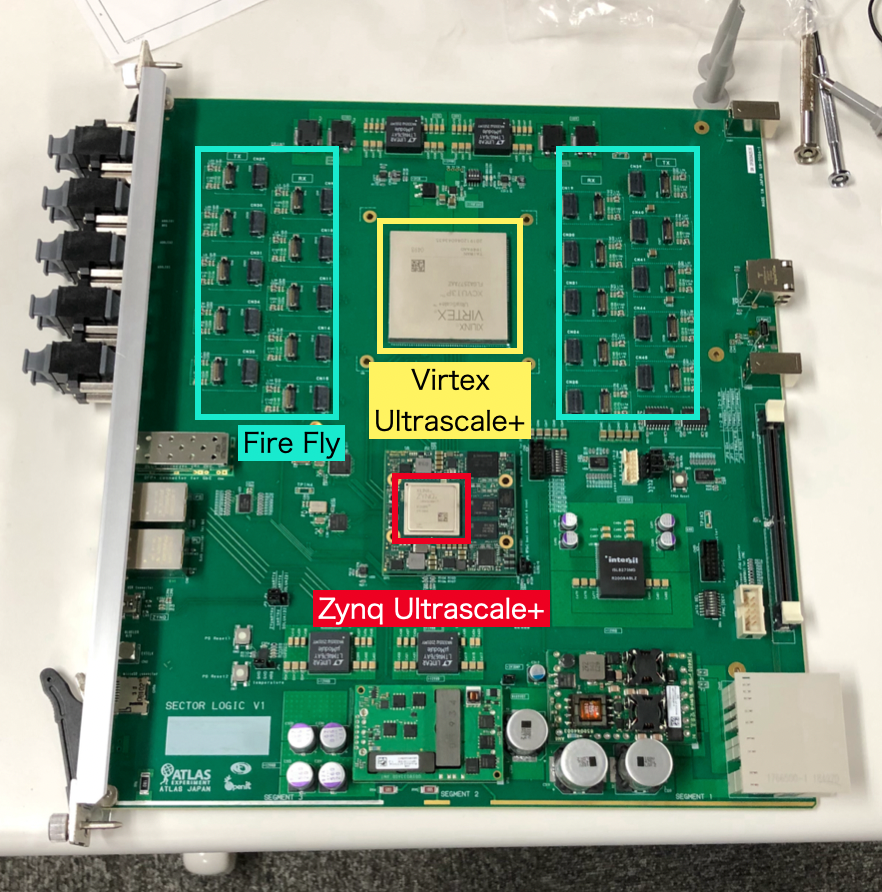
\includegraphics[width=14cm]{fig/Intro/TGC_SL.jpg}
    \caption[SL第一試作機の写真]{SL第一試作機の写真。Virtex UltraScale+ FPGAとZynq UltraScale+ MPSoCという2種類の集積回路を搭載している。他のモジュールとのインターフェイスとして、FireFlyを送信用に10個、受信用に10個搭載している。1つのFireFlyは12リンクを束ねるため、合計120リンクの光通信が可能である。}
    \label{TGC_SL}
\end{figure}

SLの第一試作機の写真を図\ref{TGC_SL}に示す。
SLはAdvanced Telecommunications Computing Architecture (ATCA)規格のボードである。ユーザーはATCAクレートのShelf managerからCERNで開発されたIntelligent Platform Management Controller  (IPMC) カードを介して、SLの電圧や温度のモニターや遠隔での電源操作を行うことができる。SLは外部とのインターフェイスとして電気信号を光信号に変換するためのFireFlyを送信用に10個、受信用に10個搭載している。それぞれが12レーンを束ねるため、送受信120リンクの光通信が可能である。1GイーサーネットケーブルのインターフェイスであるRJ45コネクターも搭載しており、イーサーネットを介したネットワーク通信も可能である。

1枚のSLはTGCの1/24セクターからの信号処理を担当し、合計31台のPS boardと接続する (BW用に29 枚、EI用に2 枚)。AsideとCsideを合わせて、合計で48枚のSLが設置される。以下にそれぞれの集積回路の機能の詳細を述べる。

    \subsubsection{SL FPGA}
SL FPGAに実装するファームウェアの概要を図\ref{SL_FW_overview}に示す。ファームウェアは大別してトリガー回路、読み出し回路、コントロール回路に分けられる。PS boardから光リンクを経由して送られるヒット情報は、トリガー回路および読み出し回路に入れられる。

\begin{figure} 
\centering
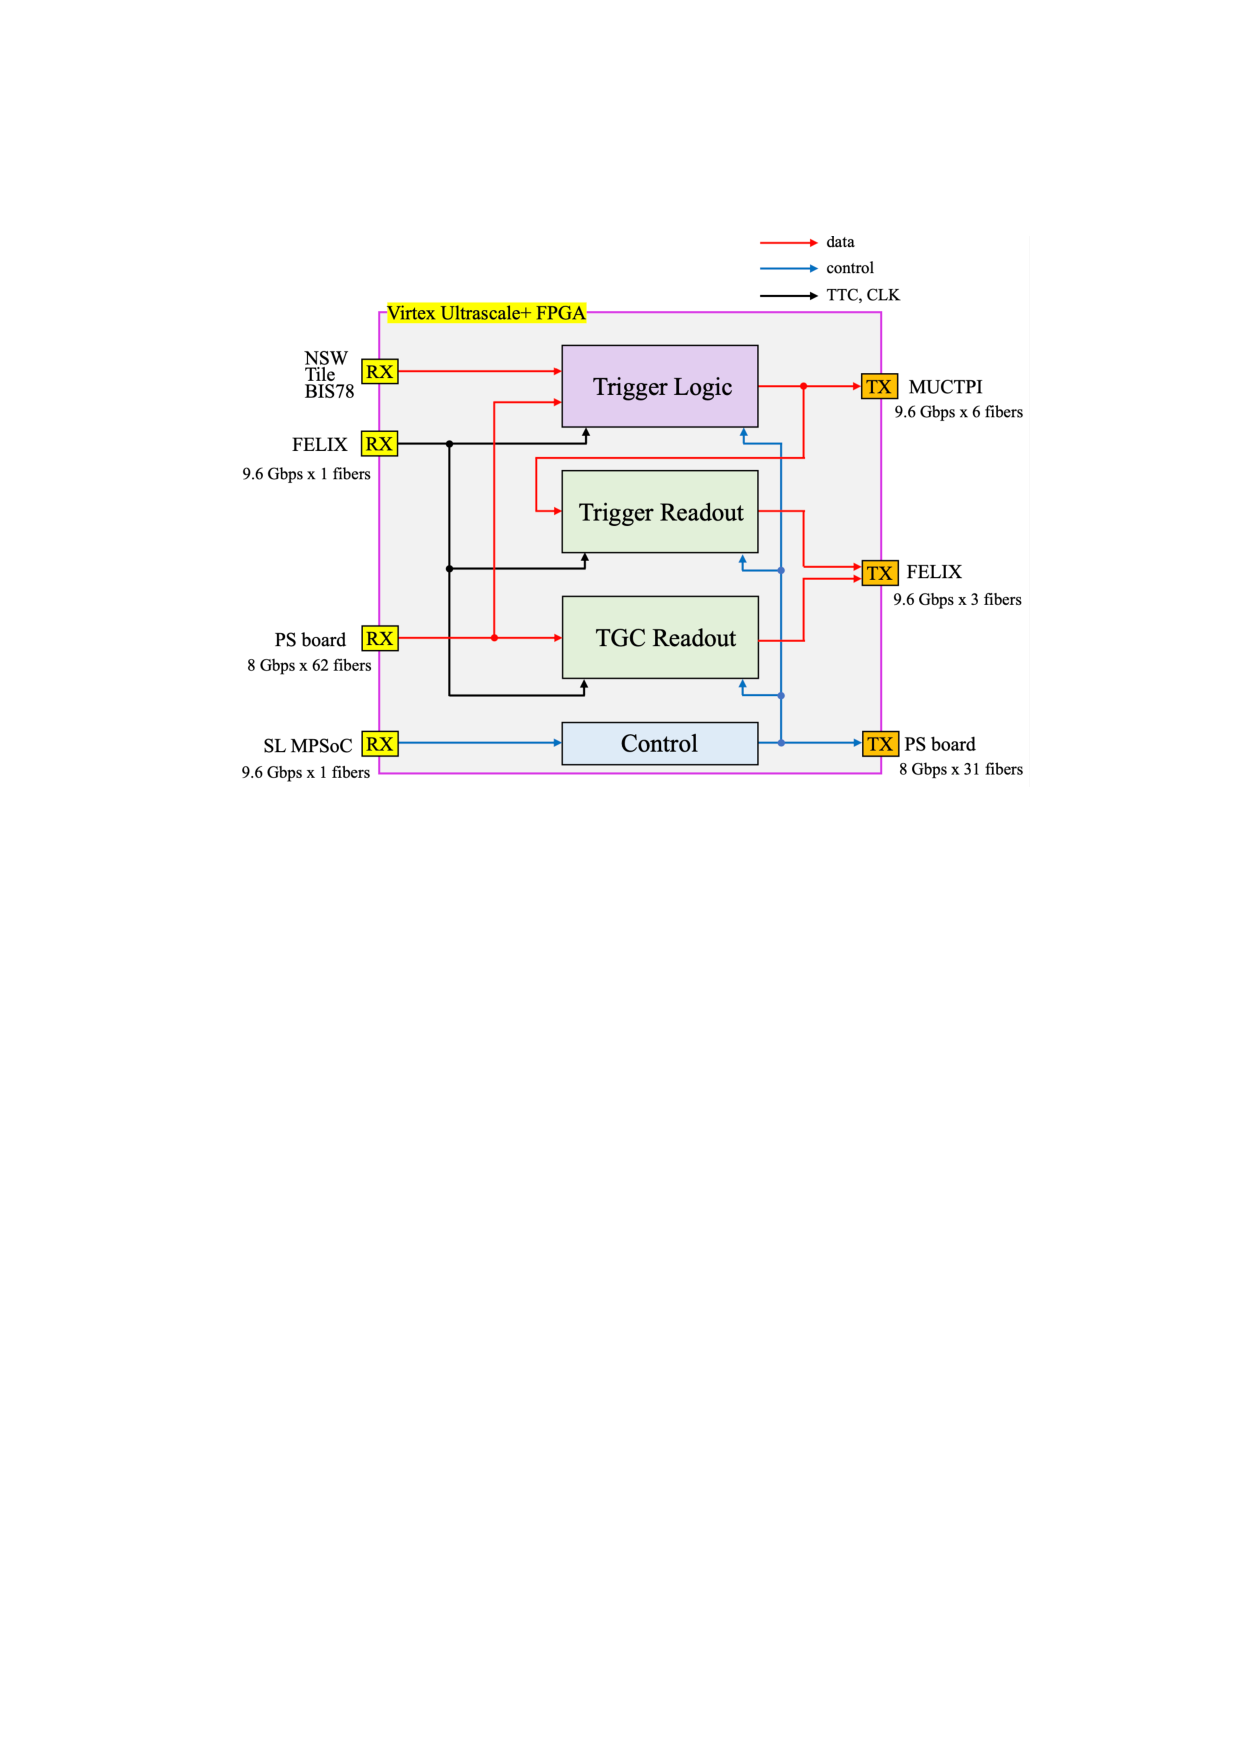
\includegraphics[width=16cm]{fig/Intro/SL_FW_overview.pdf}
\caption[SL FPGAに実装されるファームウェアの概要]{SL FPGAに実装されるファームウェアの概要\cite{mt_mishima}。SL FPGAは大別してトリガー回路、読み出し回路、コントロール回路に分けられる。トリガー回路はPS boardや磁場内部に位置する検出器からのヒットデータを受け取り、トリガー出力をMUCTPIに送信する。読み出し回路はPS boardからのヒットデータをバッファーし、FELIXからL0Aが出されたイベントのデータを取り出し、FELIXに送信する。コントロール回路はSL MPSoCからコントロール用信号を受け取り、各ロジックの制御を行う。}
\label{SL_FW_overview}
\end{figure}

トリガー回路は、PS boardから送られるBW 7層分のヒットデータを用いて\pt 判定を行なった後、エンドキャップトロイド磁石より内側にあるNSW、RPC BIS78、TIleカロリメーターからの情報も用いて、より精度の高い\pt の概算を行う。
SLで再構成されたミューオン飛跡の一部は、より精度の高い\pt 計算のためMDTTPへ送信される。MDTTPで処理された飛跡情報は、SLに送り返され、MDTTPに送られなかったものと合わせてMUCTPIへ送信される。
トリガー回路はこれまでにATLAS TGC グループの共同研究として開発が進められてきた。本研究では開発されたトリガーモジュールの全体ファームウェアへの統合および試験システムの開発を行った。この詳細は\ref{chap_TriggerIntegration}章、\ref{chap_TriggerTest}章で議論する。

読み出し回路は、PS board から受信したヒットビットマップとそのイベントに対応するトリガーデータをバッファーしておき、L0A が発行されたイベントのデータを選択的に後段へ転送する役割を担う。読み出されるデータにはゼロサプレスという圧縮処理が行われ、すべてのPS boardからのデータはイベントごとにパッキング  (Event Building) され、FELIXに送られる

コントロール回路は、LHC バンチ交差クロックと同期する必要のないスローな制御を担当する。MPSoCを起点にSL FPGA内のレジスタを操作することで、SLのトリガー・読み出しに関連するパラメーターの設定や、PS boardの制御を行う。

SL FPGAは4つのシリコンダイ (Super Logic Region, SLR) で構成される大規模なFPGAである。図\ref{ISEE_abstract}に示すように、隣接するSLRはSuper Long Line (SLL) と呼ばれる専用のワイヤーで接続されており、これを通じて信号の送受信が行われる。しかし、SLLを介した信号の伝搬は通常よりも大きなレイテンシーが生じる。さらに、SLLの位置はSLR内で物理的に固定されているため、SLLを過剰に使用する設計ではタイミング制約を満たすことが難しくなる。ファームウェアを物理的な制約 (タイミング制約やリソース使用量など) を満たしつつ効果的に実装するためには、I/Oや各種ロジックをFPGA上の適切な場所へ配置することが重要となる。

\begin{figure} 
\centering
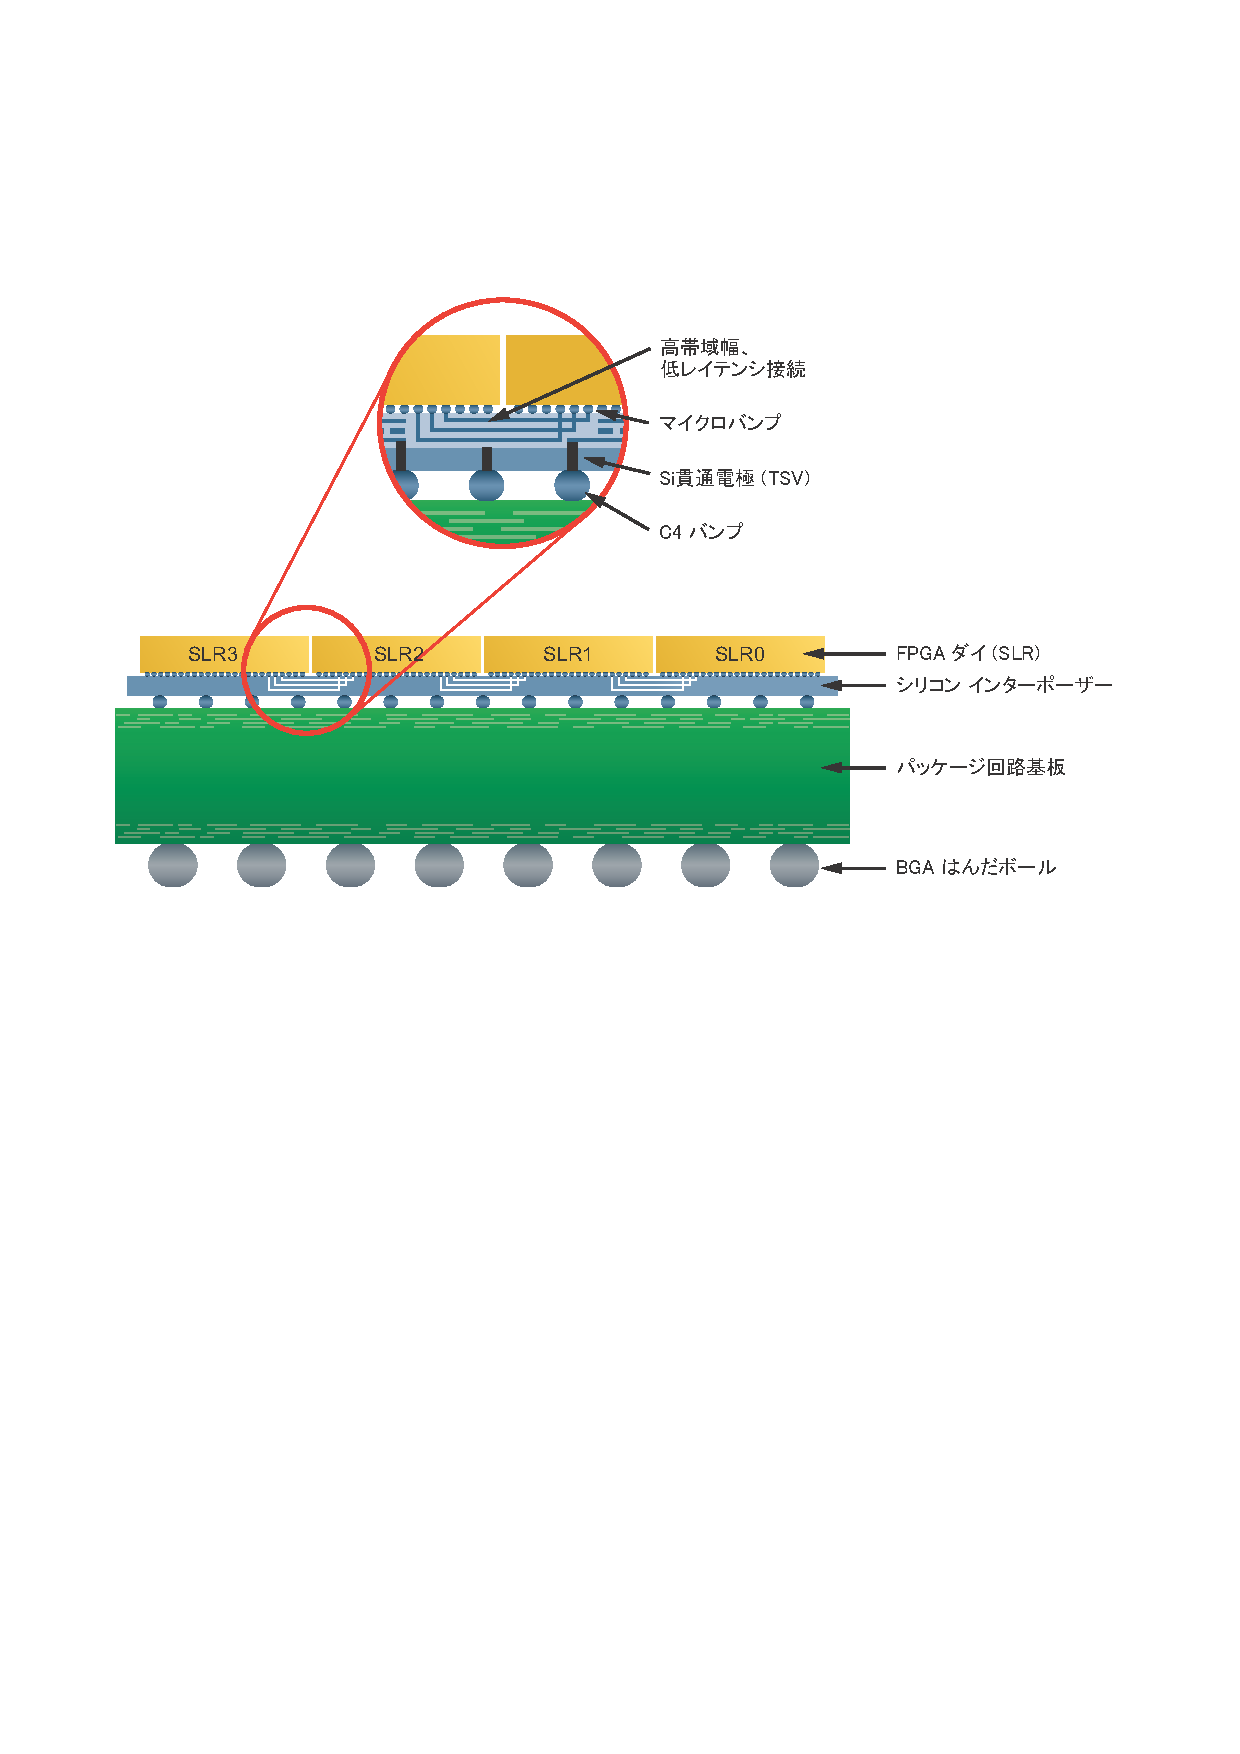
\includegraphics[width=16cm]{fig/Intro/ISEE_abstract.pdf}
\caption[SLRの概略図]{SLRの概略図。SL FPGAは4つのSLRで構成されており、隣接するSLRはSLLで接続されている。これによりSLR間で信号を送受信することができる。}
\label{ISEE_abstract}
\end{figure}

図\ref{SL_floor}に設計されたSL FPGAのフロアマッピングを示す。PS boardからのヒット信号はSLR 0、SLR 2、SLR 3で受信され、磁場内部の検出器からの信号はSLR 1で受信される。この配置に基づき、TGCのヒット信号のみを使用するトリガーロジック (TGC BW Coincidence) はそれぞれのSLRに配置され、Inner CoincidenceはSLR 1に配置される。これにより、8,000 bit に及ぶPS board からのヒット信号はそれぞれのSLRで十分にデータ量が削減された後、SLRを跨いで送信される。
TGC BW CoincidenceはトリガーセクターごとにSLRを分けて配置され、SLR 0にエンドキャップ$\phi\,0$、SLR 2にエンドキャップ$\phi\,1$、SLR 3にフォワード領域のコインシデンスロジックが配置される。

SLからFELIXにヒットデータを送信するリンクはSLR 3に配置される。SLRを超える信号をできるだけ小さくするため、読み出し回路はZero Suppressなどのデータ圧縮処理をそれぞれのSLR内で行い、SLR 3で各SLRからのヒット信号を集め、イベントごとにパッキングする。また、MPSoCとSL FPGA間のチップ間通信リンクもSLR 3に実装され、各SLRのレジスタ操作はSLR 3を介して行われる。読み出し回路やコントロール回路などのFixed latencyでの実装が求められていないロジックでは、キューイングを適用しリソースを十分に節約している。

\begin{figure} 
\centering
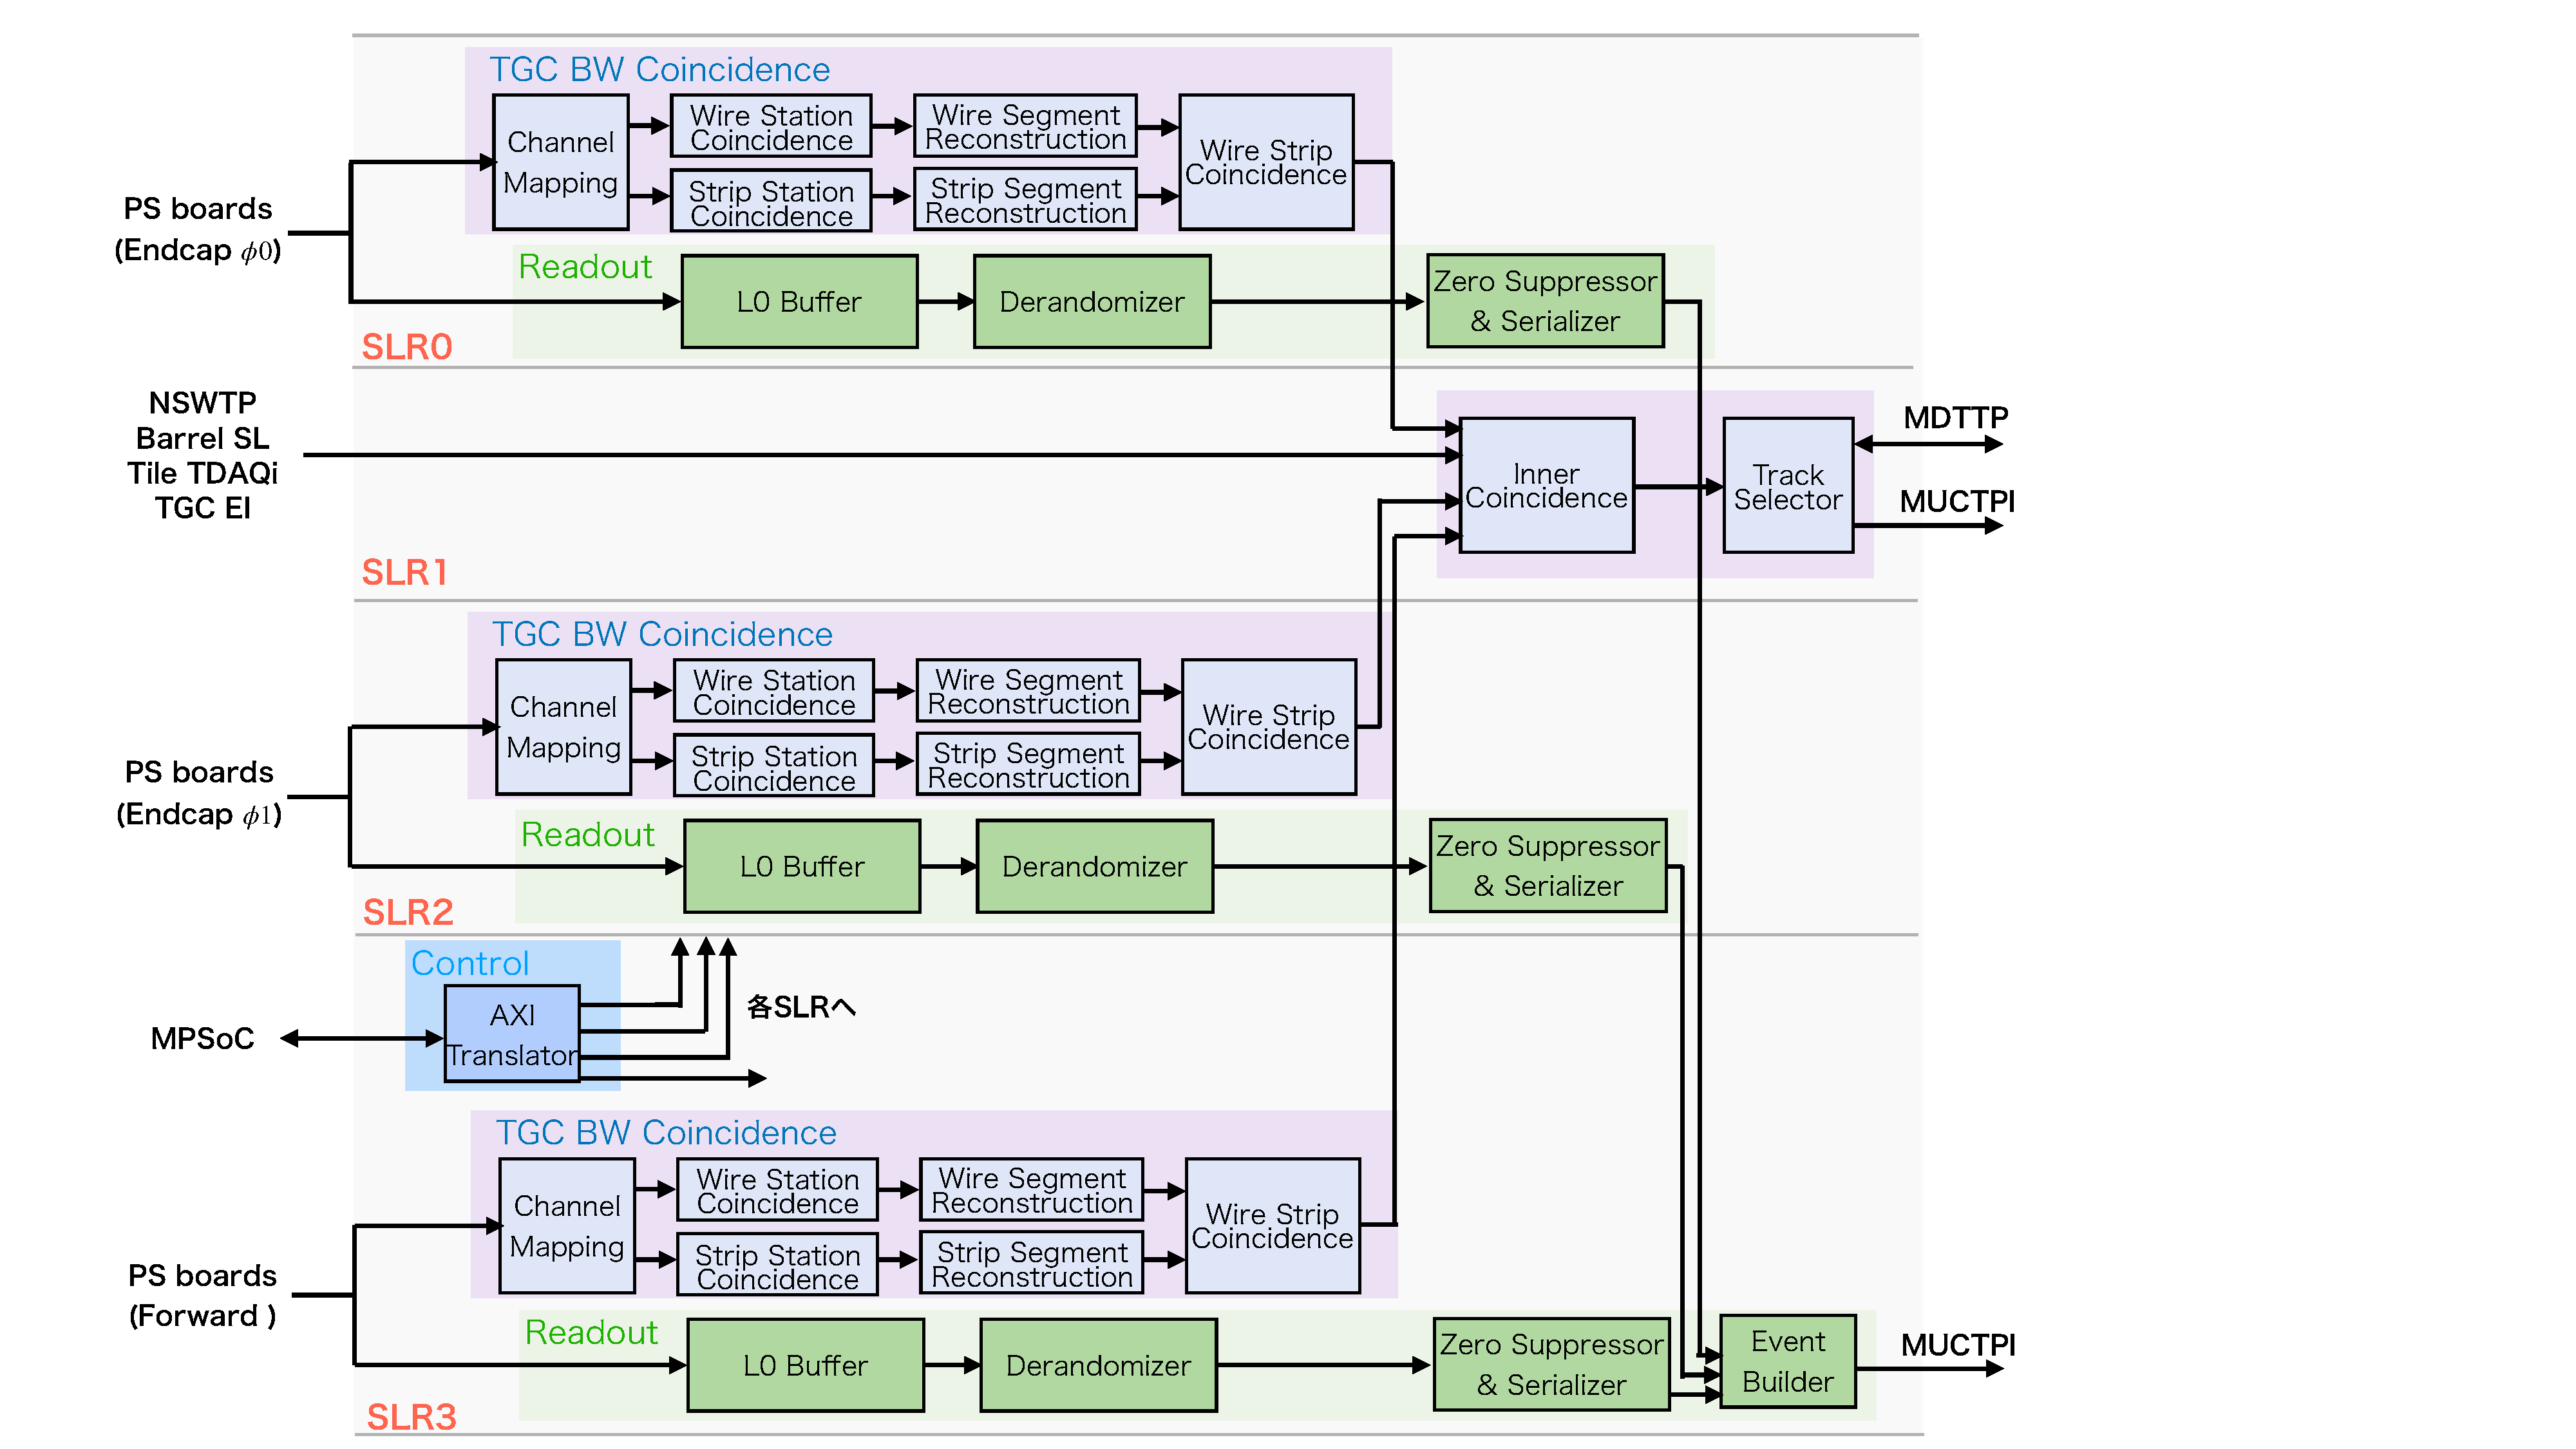
\includegraphics[width=16cm]{fig/Intro/SL_floor.pdf}
\caption[SL FPGAのフロアマップ]{SL FPGAのフロアマップ。PS boardからのヒット信号はSLR 0、SLR 2、SLR 3で受信し、磁場内部の検出器からの飛跡情報はSLR 1で受信する。それに合わせてSLR 0、2、3にはTGC BW Coincidenceおよび読み出し回路の一部を配置し、SLR 1にはInner Coincidenceを配置する。MPSoCとのインターフェイスはSLR 3に配置し、これを介して各SLR内のレジスタ操作を行う。}
\label{SL_floor}
\end{figure}



    \subsubsection*{Zynq MPSoC}
Zynq MPSoCはSL FPGAおよびPS boardのコントロールマスターとして動作する。加えてATLASのTDAQシステムやDetector Control System (DCS)とのインターフェイスとしての役割も果たす。
Zynq MPSoCもPSとPLから構成されるシリコンデバイスである。PSにはプロセッサやメモリが搭載されていて、SLでは標準的なOSであるCentOS 7を起動する。\footnote{Run 4で使用するOSは今後選定される。}

SLのMPSoCはEnclustra社が開発しているMercury XC5メザニンカードに搭載されている。このメザニンには高速通信を行うためのIOが搭載されており、SL FPGAとMPSoCは2レーンの高速シリアル通信を行うことができる。これを利用して、MPSoCからSL FPGAのコントロールや、SL FPGAからMPSoCへのデータ読み出しを行なっている。
Mercury XU5には他にも、DDR4 SDRAMやeMMC、Gigabit Ethernet PHY、USB PHY、QSPI フラッシュメモリなどが搭載されている。市販のメザニンを活用することで、SLボードの開発コストを下げることに加え、メンテナンスを容易にすることができる。Mercury XU5メザニンカードの構造と、SLボード上における接続関係を図\ref{SL_mezanin}に示す。

\begin{figure} 
\centering
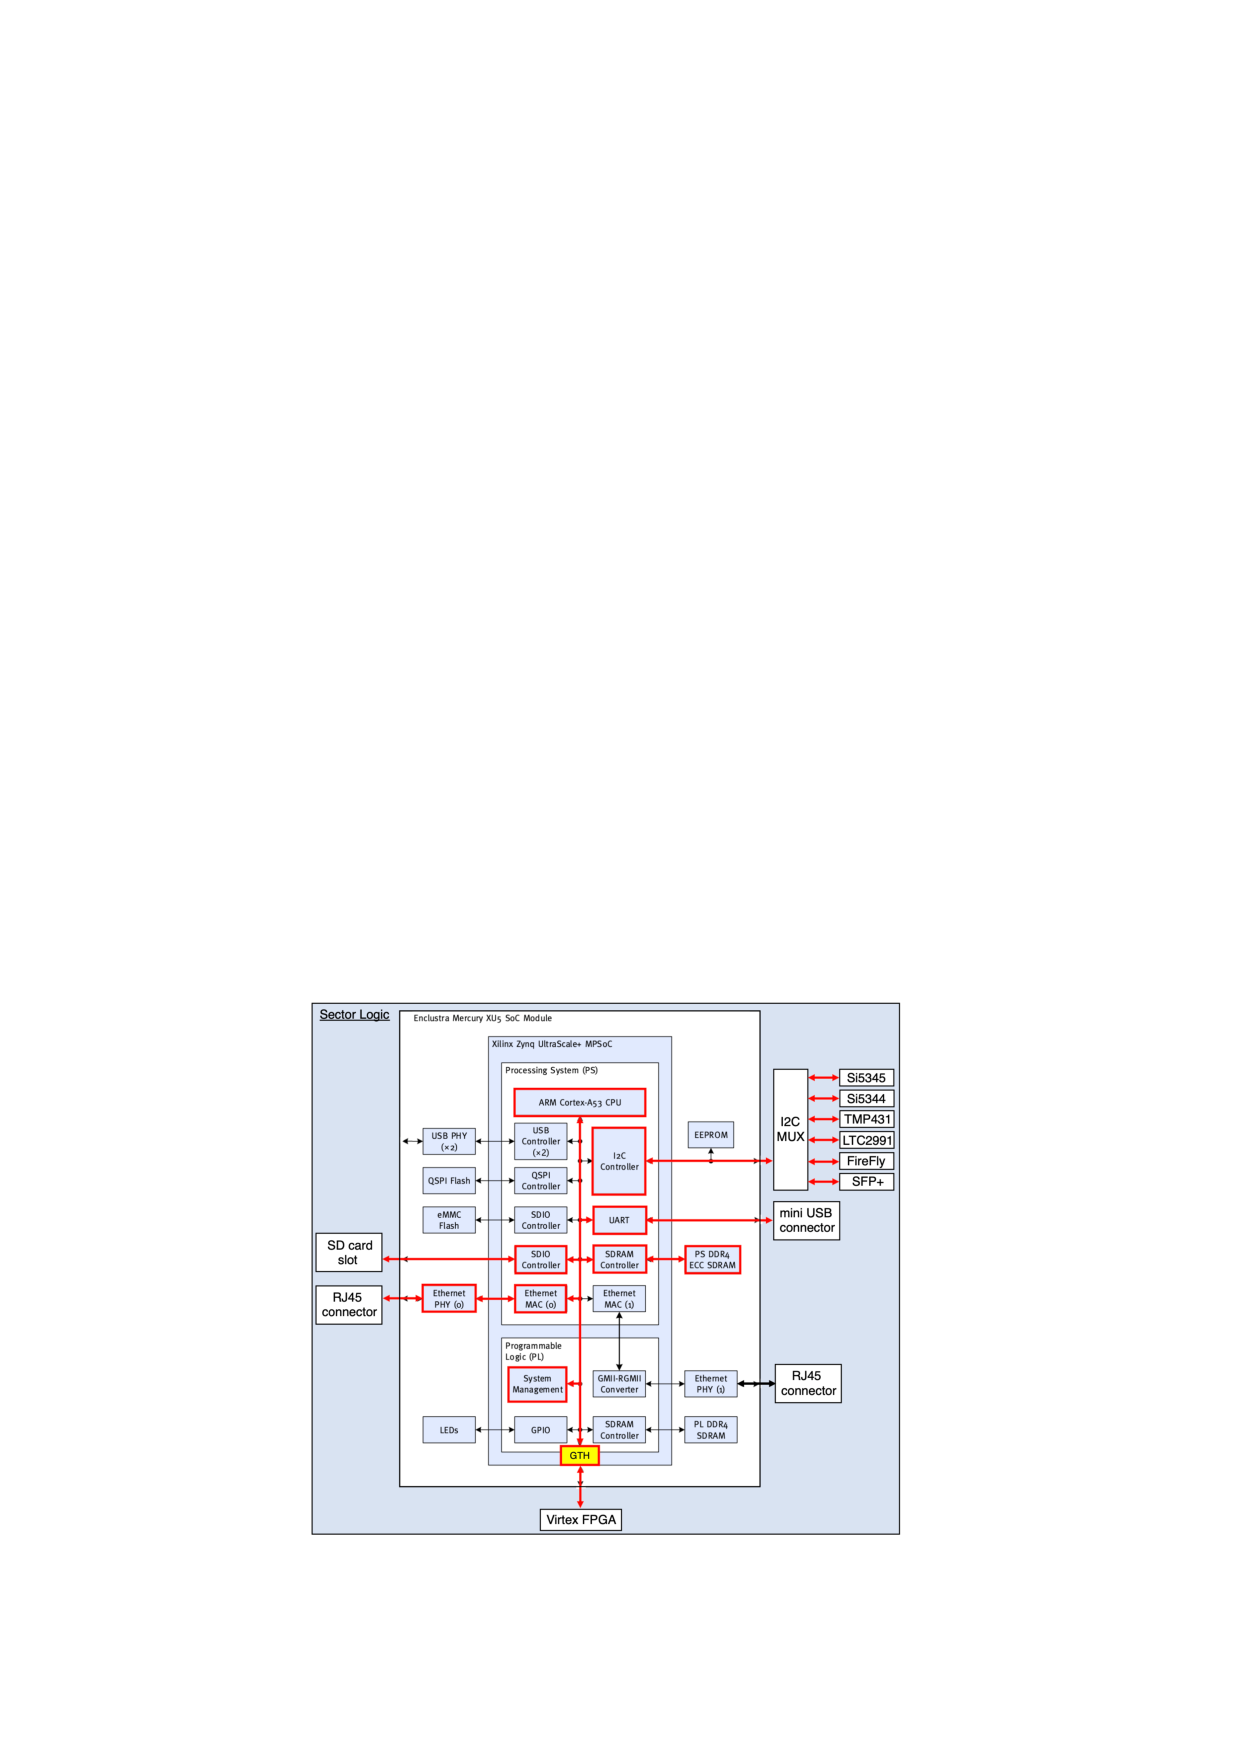
\includegraphics[width=16cm]{fig/Intro/SL_mezanin.pdf}
\caption[Mercury XU5 メザニンカードの構造とSLボード上における接続関係]{Mercury XU5 メザニンカードの構造とSLボード上における接続関係\cite{mt_mishima}}
\label{SL_mezanin}
\end{figure}